\documentclass[twoside]{book}

% Packages required by doxygen
\usepackage{fixltx2e}
\usepackage{calc}
\usepackage{doxygen}
\usepackage[export]{adjustbox} % also loads graphicx
\usepackage{graphicx}
\usepackage[utf8]{inputenc}
\usepackage{makeidx}
\usepackage{multicol}
\usepackage{multirow}
\PassOptionsToPackage{warn}{textcomp}
\usepackage{textcomp}
\usepackage[nointegrals]{wasysym}
\usepackage[table]{xcolor}

% Font selection
\usepackage[T1]{fontenc}
\usepackage[scaled=.90]{helvet}
\usepackage{courier}
\usepackage{amssymb}
\usepackage{sectsty}
\renewcommand{\familydefault}{\sfdefault}
\allsectionsfont{%
  \fontseries{bc}\selectfont%
  \color{darkgray}%
}
\renewcommand{\DoxyLabelFont}{%
  \fontseries{bc}\selectfont%
  \color{darkgray}%
}
\newcommand{\+}{\discretionary{\mbox{\scriptsize$\hookleftarrow$}}{}{}}

% Page & text layout
\usepackage{geometry}
\geometry{%
  a4paper,%
  top=2.5cm,%
  bottom=2.5cm,%
  left=2.5cm,%
  right=2.5cm%
}
\tolerance=750
\hfuzz=15pt
\hbadness=750
\setlength{\emergencystretch}{15pt}
\setlength{\parindent}{0cm}
\setlength{\parskip}{3ex plus 2ex minus 2ex}
\makeatletter
\renewcommand{\paragraph}{%
  \@startsection{paragraph}{4}{0ex}{-1.0ex}{1.0ex}{%
    \normalfont\normalsize\bfseries\SS@parafont%
  }%
}
\renewcommand{\subparagraph}{%
  \@startsection{subparagraph}{5}{0ex}{-1.0ex}{1.0ex}{%
    \normalfont\normalsize\bfseries\SS@subparafont%
  }%
}
\makeatother

% Headers & footers
\usepackage{fancyhdr}
\pagestyle{fancyplain}
\fancyhead[LE]{\fancyplain{}{\bfseries\thepage}}
\fancyhead[CE]{\fancyplain{}{}}
\fancyhead[RE]{\fancyplain{}{\bfseries\leftmark}}
\fancyhead[LO]{\fancyplain{}{\bfseries\rightmark}}
\fancyhead[CO]{\fancyplain{}{}}
\fancyhead[RO]{\fancyplain{}{\bfseries\thepage}}
\fancyfoot[LE]{\fancyplain{}{}}
\fancyfoot[CE]{\fancyplain{}{}}
\fancyfoot[RE]{\fancyplain{}{\bfseries\scriptsize Generated by Doxygen }}
\fancyfoot[LO]{\fancyplain{}{\bfseries\scriptsize Generated by Doxygen }}
\fancyfoot[CO]{\fancyplain{}{}}
\fancyfoot[RO]{\fancyplain{}{}}
\renewcommand{\footrulewidth}{0.4pt}
\renewcommand{\chaptermark}[1]{%
  \markboth{#1}{}%
}
\renewcommand{\sectionmark}[1]{%
  \markright{\thesection\ #1}%
}

% Indices & bibliography
\usepackage{natbib}
\usepackage[titles]{tocloft}
\setcounter{tocdepth}{3}
\setcounter{secnumdepth}{5}
\makeindex

% Hyperlinks (required, but should be loaded last)
\usepackage{ifpdf}
\ifpdf
  \usepackage[pdftex,pagebackref=true]{hyperref}
\else
  \usepackage[ps2pdf,pagebackref=true]{hyperref}
\fi
\hypersetup{%
  colorlinks=true,%
  linkcolor=blue,%
  citecolor=blue,%
  unicode%
}

% Custom commands
\newcommand{\clearemptydoublepage}{%
  \newpage{\pagestyle{empty}\cleardoublepage}%
}

\usepackage{caption}
\captionsetup{labelsep=space,justification=centering,font={bf},singlelinecheck=off,skip=4pt,position=top}

%===== C O N T E N T S =====

\begin{document}

% Titlepage & ToC
\hypersetup{pageanchor=false,
             bookmarksnumbered=true,
             pdfencoding=unicode
            }
\pagenumbering{roman}
\begin{titlepage}
\vspace*{7cm}
\begin{center}%
{\Large C\+A\+D-\/\+Tool }\\
\vspace*{1cm}
{\large Generated by Doxygen 1.8.11}\\
\end{center}
\end{titlepage}
\clearemptydoublepage
\tableofcontents
\clearemptydoublepage
\pagenumbering{arabic}
\hypersetup{pageanchor=true}

%--- Begin generated contents ---
\chapter{C\+O\+P290 -\/ Orthographic views of a solid and Reconstruction of Solid from given orthographic projections -\/ Documentation}
\label{index}\hypertarget{index}{}\hypertarget{index_intro_sec}{}\section{I\+N\+T\+R\+O\+D\+U\+C\+T\+I\+ON}\label{index_intro_sec}
The objective of this project is to design and implement a software package which reconstructs a 3-\/D object from its given orthographic views and from the given 3-\/D object gives its projections on a given cutting plane and its orthographic views(top, front, right side view). This document mainly talks about the mathematical model involved in this project and the algorithms to achieve the same. In this project we are considering only polyhedron 3-\/D objects which have flat polygon faces. For reconstruction of any polyhedron object, 3 orthographic views are sufficient and 2 orthographic views are necessary as some symmetric polyhedron objects can be uniquely reconstructed from 2 orthographic views.\hypertarget{index_assumption_sec}{}\section{A\+S\+S\+U\+M\+P\+T\+I\+O\+NS}\label{index_assumption_sec}
\hypertarget{index_subsection1}{}\subsection{3\+D to 2\+D Transformation -\/}\label{index_subsection1}
The projected views provided in the input are top view, front view and right side view of the object. Hidden lines are also treated as solid lines. \hypertarget{index_subsection2}{}\subsection{2\+D to 3\+D Transformation -\/}\label{index_subsection2}
Hidden lines also being shown as solid lines. The information provided about the object forms a valid 3D object. Provided projection forms a valid object. 
\chapter{Namespace Index}
\section{Namespace List}
Here is a list of all namespaces with brief descriptions\+:\begin{DoxyCompactList}
\item\contentsline{section}{\hyperlink{namespace_ui}{Ui} }{\pageref{namespace_ui}}{}
\end{DoxyCompactList}

\chapter{Hierarchical Index}
\section{Class Hierarchy}
This inheritance list is sorted roughly, but not completely, alphabetically\+:\begin{DoxyCompactList}
\item \contentsline{section}{basic\+\_\+loop}{\pageref{classbasic__loop}}{}
\item \contentsline{section}{body\+\_\+loop}{\pageref{classbody__loop}}{}
\item \contentsline{section}{edge\+\_\+2d}{\pageref{classedge__2d}}{}
\item \contentsline{section}{edge\+\_\+2d\+\_\+v2v}{\pageref{classedge__2d__v2v}}{}
\item \contentsline{section}{edge\+\_\+3d}{\pageref{classedge__3d}}{}
\item \contentsline{section}{face\+\_\+loop}{\pageref{classface__loop}}{}
\item \contentsline{section}{Full\+\_\+plane}{\pageref{class_full__plane}}{}
\item \contentsline{section}{Object3d}{\pageref{class_object3d}}{}
\item \contentsline{section}{object\+\_\+2d}{\pageref{classobject__2d}}{}
\item \contentsline{section}{Object\+\_\+3d}{\pageref{class_object__3d}}{}
\item \contentsline{section}{plane}{\pageref{classplane}}{}
\item Q\+Main\+Window\begin{DoxyCompactList}
\item \contentsline{section}{Main\+Window}{\pageref{class_main_window}}{}
\end{DoxyCompactList}
\item Q\+Widget\begin{DoxyCompactList}
\item \contentsline{section}{Form}{\pageref{class_form}}{}
\end{DoxyCompactList}
\item \contentsline{section}{vertex\+\_\+2d}{\pageref{classvertex__2d}}{}
\item \contentsline{section}{vertex\+\_\+3d}{\pageref{classvertex__3d}}{}
\end{DoxyCompactList}

\chapter{Class Index}
\section{Class List}
Here are the classes, structs, unions and interfaces with brief descriptions\+:\begin{DoxyCompactList}
\item\contentsline{section}{\hyperlink{classbasic__loop}{basic\+\_\+loop} }{\pageref{classbasic__loop}}{}
\item\contentsline{section}{\hyperlink{classbody__loop}{body\+\_\+loop} }{\pageref{classbody__loop}}{}
\item\contentsline{section}{\hyperlink{classedge__2d}{edge\+\_\+2d} \\*Class for an \hyperlink{classedge__2d}{edge\+\_\+2d} }{\pageref{classedge__2d}}{}
\item\contentsline{section}{\hyperlink{classedge__2d__v2v}{edge\+\_\+2d\+\_\+v2v} \\*Class for an \hyperlink{classedge__2d__v2v}{edge\+\_\+2d\+\_\+v2v} }{\pageref{classedge__2d__v2v}}{}
\item\contentsline{section}{\hyperlink{classedge__3d}{edge\+\_\+3d} \\*Class for an \hyperlink{classedge__3d}{edge\+\_\+3d} }{\pageref{classedge__3d}}{}
\item\contentsline{section}{\hyperlink{classface__loop}{face\+\_\+loop} }{\pageref{classface__loop}}{}
\item\contentsline{section}{\hyperlink{class_form}{Form} }{\pageref{class_form}}{}
\item\contentsline{section}{\hyperlink{class_full__plane}{Full\+\_\+plane} }{\pageref{class_full__plane}}{}
\item\contentsline{section}{\hyperlink{class_main_window}{Main\+Window} }{\pageref{class_main_window}}{}
\item\contentsline{section}{\hyperlink{class_object3d}{Object3d} \\*Class for representation of a 3D object }{\pageref{class_object3d}}{}
\item\contentsline{section}{\hyperlink{classobject__2d}{object\+\_\+2d} \\*Representation of \hyperlink{classobject__2d}{object\+\_\+2d} }{\pageref{classobject__2d}}{}
\item\contentsline{section}{\hyperlink{class_object__3d}{Object\+\_\+3d} }{\pageref{class_object__3d}}{}
\item\contentsline{section}{\hyperlink{classplane}{plane} \\*Class for a plane plane represented as (a,b,c,d) corresponding to the equation ax + by + cz = d }{\pageref{classplane}}{}
\item\contentsline{section}{\hyperlink{classvertex__2d}{vertex\+\_\+2d} \\*Class for a \hyperlink{classvertex__2d}{vertex\+\_\+2d} }{\pageref{classvertex__2d}}{}
\item\contentsline{section}{\hyperlink{classvertex__3d}{vertex\+\_\+3d} \\*Class for a \hyperlink{classvertex__3d}{vertex\+\_\+3d} }{\pageref{classvertex__3d}}{}
\end{DoxyCompactList}

\chapter{File Index}
\section{File List}
Here is a list of all files with brief descriptions\+:\begin{DoxyCompactList}
\item\contentsline{section}{\hyperlink{2d__to__3d_8h}{2d\+\_\+to\+\_\+3d.\+h} }{\pageref{2d__to__3d_8h}}{}
\item\contentsline{section}{\hyperlink{3d__to__2d_8h}{3d\+\_\+to\+\_\+2d.\+h} }{\pageref{3d__to__2d_8h}}{}
\item\contentsline{section}{\hyperlink{body__loop_8h}{body\+\_\+loop.\+h} }{\pageref{body__loop_8h}}{}
\item\contentsline{section}{\hyperlink{faceloop__generator_8h}{faceloop\+\_\+generator.\+h} }{\pageref{faceloop__generator_8h}}{}
\item\contentsline{section}{\hyperlink{form_8h}{form.\+h} }{\pageref{form_8h}}{}
\item\contentsline{section}{\hyperlink{_full__plane_8h}{Full\+\_\+plane.\+h} }{\pageref{_full__plane_8h}}{}
\item\contentsline{section}{\hyperlink{general__methods_8h}{general\+\_\+methods.\+h} }{\pageref{general__methods_8h}}{}
\item\contentsline{section}{\hyperlink{mainwindow_8h}{mainwindow.\+h} }{\pageref{mainwindow_8h}}{}
\item\contentsline{section}{\hyperlink{object__2d_8h}{object\+\_\+2d.\+h} }{\pageref{object__2d_8h}}{}
\item\contentsline{section}{\hyperlink{_object__3d_8h}{Object\+\_\+3d.\+h} }{\pageref{_object__3d_8h}}{}
\item\contentsline{section}{\hyperlink{planar__graph__generator_8h}{planar\+\_\+graph\+\_\+generator.\+h} }{\pageref{planar__graph__generator_8h}}{}
\item\contentsline{section}{\hyperlink{structs_8h}{structs.\+h} }{\pageref{structs_8h}}{}
\item\contentsline{section}{/home/manish/\+Desktop/\+Manish\+\_\+\+C\+A\+D\+\_\+\+Tool/src/\hyperlink{2d__to__3d_8cpp}{2d\+\_\+to\+\_\+3d.\+cpp} }{\pageref{2d__to__3d_8cpp}}{}
\item\contentsline{section}{/home/manish/\+Desktop/\+Manish\+\_\+\+C\+A\+D\+\_\+\+Tool/src/\hyperlink{3d__to__2d_8cpp}{3d\+\_\+to\+\_\+2d.\+cpp} }{\pageref{3d__to__2d_8cpp}}{}
\item\contentsline{section}{/home/manish/\+Desktop/\+Manish\+\_\+\+C\+A\+D\+\_\+\+Tool/src/\hyperlink{body__loop_8cpp}{body\+\_\+loop.\+cpp} }{\pageref{body__loop_8cpp}}{}
\item\contentsline{section}{/home/manish/\+Desktop/\+Manish\+\_\+\+C\+A\+D\+\_\+\+Tool/src/\hyperlink{faceloop__generator_8cpp}{faceloop\+\_\+generator.\+cpp} }{\pageref{faceloop__generator_8cpp}}{}
\item\contentsline{section}{/home/manish/\+Desktop/\+Manish\+\_\+\+C\+A\+D\+\_\+\+Tool/src/\hyperlink{form_8cpp}{form.\+cpp} }{\pageref{form_8cpp}}{}
\item\contentsline{section}{/home/manish/\+Desktop/\+Manish\+\_\+\+C\+A\+D\+\_\+\+Tool/src/\hyperlink{_full__plane_8cpp}{Full\+\_\+plane.\+cpp} }{\pageref{_full__plane_8cpp}}{}
\item\contentsline{section}{/home/manish/\+Desktop/\+Manish\+\_\+\+C\+A\+D\+\_\+\+Tool/src/\hyperlink{general__methods_8cpp}{general\+\_\+methods.\+cpp} }{\pageref{general__methods_8cpp}}{}
\item\contentsline{section}{/home/manish/\+Desktop/\+Manish\+\_\+\+C\+A\+D\+\_\+\+Tool/src/\hyperlink{main_8cpp}{main.\+cpp} }{\pageref{main_8cpp}}{}
\item\contentsline{section}{/home/manish/\+Desktop/\+Manish\+\_\+\+C\+A\+D\+\_\+\+Tool/src/\hyperlink{mainwindow_8cpp}{mainwindow.\+cpp} }{\pageref{mainwindow_8cpp}}{}
\item\contentsline{section}{/home/manish/\+Desktop/\+Manish\+\_\+\+C\+A\+D\+\_\+\+Tool/src/\hyperlink{object__2d_8cpp}{object\+\_\+2d.\+cpp} }{\pageref{object__2d_8cpp}}{}
\item\contentsline{section}{/home/manish/\+Desktop/\+Manish\+\_\+\+C\+A\+D\+\_\+\+Tool/src/\hyperlink{_object__3d_8cpp}{Object\+\_\+3d.\+cpp} }{\pageref{_object__3d_8cpp}}{}
\item\contentsline{section}{/home/manish/\+Desktop/\+Manish\+\_\+\+C\+A\+D\+\_\+\+Tool/src/\hyperlink{planar__graph__generator_8cpp}{planar\+\_\+graph\+\_\+generator.\+cpp} }{\pageref{planar__graph__generator_8cpp}}{}
\item\contentsline{section}{/home/manish/\+Desktop/\+Manish\+\_\+\+C\+A\+D\+\_\+\+Tool/src/\hyperlink{structs_8cpp}{structs.\+cpp} }{\pageref{structs_8cpp}}{}
\end{DoxyCompactList}

\chapter{Namespace Documentation}
\hypertarget{namespace_ui}{}\section{Ui Namespace Reference}
\label{namespace_ui}\index{Ui@{Ui}}

\chapter{Class Documentation}
\hypertarget{classbasic__loop}{}\section{basic\+\_\+loop Class Reference}
\label{classbasic__loop}\index{basic\+\_\+loop@{basic\+\_\+loop}}


{\ttfamily \#include $<$faceloop\+\_\+generator.\+h$>$}

\subsection*{Public Member Functions}
\begin{DoxyCompactItemize}
\item 
\hyperlink{classbasic__loop_a400c87feeca18d4e1c5885adccc5b3a1}{basic\+\_\+loop} (std\+::vector$<$ \hyperlink{classedge__3d}{edge\+\_\+3d} $>$ loop, bool \hyperlink{classbasic__loop_a79ff39c7f385ef03176dca8c675844fe}{inner})
\begin{DoxyCompactList}\small\item\em Constructor. \end{DoxyCompactList}\end{DoxyCompactItemize}
\subsection*{Public Attributes}
\begin{DoxyCompactItemize}
\item 
std\+::vector$<$ \hyperlink{classedge__3d}{edge\+\_\+3d} $>$ \hyperlink{classbasic__loop_a81512ce2e37b1de9142568113140ace9}{edge\+\_\+list}
\begin{DoxyCompactList}\small\item\em vector of edges included in the loop \end{DoxyCompactList}\item 
bool \hyperlink{classbasic__loop_a79ff39c7f385ef03176dca8c675844fe}{inner}
\begin{DoxyCompactList}\small\item\em bool is true if loop is inner \end{DoxyCompactList}\end{DoxyCompactItemize}


\subsection{Detailed Description}


Definition at line 12 of file faceloop\+\_\+generator.\+h.



\subsection{Constructor \& Destructor Documentation}
\index{basic\+\_\+loop@{basic\+\_\+loop}!basic\+\_\+loop@{basic\+\_\+loop}}
\index{basic\+\_\+loop@{basic\+\_\+loop}!basic\+\_\+loop@{basic\+\_\+loop}}
\subsubsection[{\texorpdfstring{basic\+\_\+loop(std\+::vector$<$ edge\+\_\+3d $>$ loop, bool inner)}{basic_loop(std::vector< edge_3d > loop, bool inner)}}]{\setlength{\rightskip}{0pt plus 5cm}basic\+\_\+loop\+::basic\+\_\+loop (
\begin{DoxyParamCaption}
\item[{std\+::vector$<$ {\bf edge\+\_\+3d} $>$}]{loop, }
\item[{bool}]{inner}
\end{DoxyParamCaption}
)}\hypertarget{classbasic__loop_a400c87feeca18d4e1c5885adccc5b3a1}{}\label{classbasic__loop_a400c87feeca18d4e1c5885adccc5b3a1}


Constructor. 



Definition at line 9 of file faceloop\+\_\+generator.\+cpp.



\subsection{Member Data Documentation}
\index{basic\+\_\+loop@{basic\+\_\+loop}!edge\+\_\+list@{edge\+\_\+list}}
\index{edge\+\_\+list@{edge\+\_\+list}!basic\+\_\+loop@{basic\+\_\+loop}}
\subsubsection[{\texorpdfstring{edge\+\_\+list}{edge_list}}]{\setlength{\rightskip}{0pt plus 5cm}std\+::vector$<${\bf edge\+\_\+3d}$>$ basic\+\_\+loop\+::edge\+\_\+list}\hypertarget{classbasic__loop_a81512ce2e37b1de9142568113140ace9}{}\label{classbasic__loop_a81512ce2e37b1de9142568113140ace9}


vector of edges included in the loop 



Definition at line 15 of file faceloop\+\_\+generator.\+h.

\index{basic\+\_\+loop@{basic\+\_\+loop}!inner@{inner}}
\index{inner@{inner}!basic\+\_\+loop@{basic\+\_\+loop}}
\subsubsection[{\texorpdfstring{inner}{inner}}]{\setlength{\rightskip}{0pt plus 5cm}bool basic\+\_\+loop\+::inner}\hypertarget{classbasic__loop_a79ff39c7f385ef03176dca8c675844fe}{}\label{classbasic__loop_a79ff39c7f385ef03176dca8c675844fe}


bool is true if loop is inner 



Definition at line 16 of file faceloop\+\_\+generator.\+h.



The documentation for this class was generated from the following files\+:\begin{DoxyCompactItemize}
\item 
\hyperlink{faceloop__generator_8h}{faceloop\+\_\+generator.\+h}\item 
/home/manish/\+Desktop/\+Manish\+\_\+\+C\+A\+D\+\_\+\+Tool/src/\hyperlink{faceloop__generator_8cpp}{faceloop\+\_\+generator.\+cpp}\end{DoxyCompactItemize}

\hypertarget{classbody__loop}{}\section{body\+\_\+loop Class Reference}
\label{classbody__loop}\index{body\+\_\+loop@{body\+\_\+loop}}


{\ttfamily \#include $<$body\+\_\+loop.\+h$>$}

\subsection*{Public Member Functions}
\begin{DoxyCompactItemize}
\item 
\hyperlink{classbody__loop_af2f9c347cafb6dea337d5cdc1ae78394}{body\+\_\+loop} (std\+::vector$<$ \hyperlink{classface__loop}{face\+\_\+loop} $>$ \hyperlink{classbody__loop_aac59ff1c3fd827c48ad15391400600d4}{face\+\_\+loop\+\_\+list})
\begin{DoxyCompactList}\small\item\em Constructor. \end{DoxyCompactList}\item 
\hyperlink{classbody__loop_a01aca1cecd85e46978c47e1fc0aa5fca}{body\+\_\+loop} ()
\begin{DoxyCompactList}\small\item\em Constructor. \end{DoxyCompactList}\item 
void \hyperlink{classbody__loop_a979500fe24969e0a35906e515f6f2b18}{add\+\_\+face\+\_\+loop} (\hyperlink{classface__loop}{face\+\_\+loop} fl, bool side)
\begin{DoxyCompactList}\small\item\em function that adds face loop in the face\+\_\+loop\+\_\+list \end{DoxyCompactList}\end{DoxyCompactItemize}
\subsection*{Public Attributes}
\begin{DoxyCompactItemize}
\item 
std\+::vector$<$ \hyperlink{classface__loop}{face\+\_\+loop} $>$ \hyperlink{classbody__loop_aac59ff1c3fd827c48ad15391400600d4}{face\+\_\+loop\+\_\+list}
\begin{DoxyCompactList}\small\item\em vector of face loops included in a particular body part \end{DoxyCompactList}\item 
std\+::vector$<$ bool $>$ \hyperlink{classbody__loop_aa4e8adf7cebc6dc08ff335b71b0b6fa0}{side\+\_\+of\+\_\+face\+\_\+loop}
\begin{DoxyCompactList}\small\item\em vector of side of corresponding face loops list \end{DoxyCompactList}\end{DoxyCompactItemize}


\subsection{Detailed Description}


Definition at line 10 of file body\+\_\+loop.\+h.



\subsection{Constructor \& Destructor Documentation}
\index{body\+\_\+loop@{body\+\_\+loop}!body\+\_\+loop@{body\+\_\+loop}}
\index{body\+\_\+loop@{body\+\_\+loop}!body\+\_\+loop@{body\+\_\+loop}}
\subsubsection[{\texorpdfstring{body\+\_\+loop(std\+::vector$<$ face\+\_\+loop $>$ face\+\_\+loop\+\_\+list)}{body_loop(std::vector< face_loop > face_loop_list)}}]{\setlength{\rightskip}{0pt plus 5cm}body\+\_\+loop\+::body\+\_\+loop (
\begin{DoxyParamCaption}
\item[{std\+::vector$<$ {\bf face\+\_\+loop} $>$}]{face\+\_\+loop\+\_\+list}
\end{DoxyParamCaption}
)}\hypertarget{classbody__loop_af2f9c347cafb6dea337d5cdc1ae78394}{}\label{classbody__loop_af2f9c347cafb6dea337d5cdc1ae78394}


Constructor. 



Definition at line 14 of file body\+\_\+loop.\+cpp.

\index{body\+\_\+loop@{body\+\_\+loop}!body\+\_\+loop@{body\+\_\+loop}}
\index{body\+\_\+loop@{body\+\_\+loop}!body\+\_\+loop@{body\+\_\+loop}}
\subsubsection[{\texorpdfstring{body\+\_\+loop()}{body_loop()}}]{\setlength{\rightskip}{0pt plus 5cm}body\+\_\+loop\+::body\+\_\+loop (
\begin{DoxyParamCaption}
{}
\end{DoxyParamCaption}
)}\hypertarget{classbody__loop_a01aca1cecd85e46978c47e1fc0aa5fca}{}\label{classbody__loop_a01aca1cecd85e46978c47e1fc0aa5fca}


Constructor. 



Definition at line 22 of file body\+\_\+loop.\+cpp.



\subsection{Member Function Documentation}
\index{body\+\_\+loop@{body\+\_\+loop}!add\+\_\+face\+\_\+loop@{add\+\_\+face\+\_\+loop}}
\index{add\+\_\+face\+\_\+loop@{add\+\_\+face\+\_\+loop}!body\+\_\+loop@{body\+\_\+loop}}
\subsubsection[{\texorpdfstring{add\+\_\+face\+\_\+loop(face\+\_\+loop fl, bool side)}{add_face_loop(face_loop fl, bool side)}}]{\setlength{\rightskip}{0pt plus 5cm}void body\+\_\+loop\+::add\+\_\+face\+\_\+loop (
\begin{DoxyParamCaption}
\item[{{\bf face\+\_\+loop}}]{fl, }
\item[{bool}]{side}
\end{DoxyParamCaption}
)}\hypertarget{classbody__loop_a979500fe24969e0a35906e515f6f2b18}{}\label{classbody__loop_a979500fe24969e0a35906e515f6f2b18}


function that adds face loop in the face\+\_\+loop\+\_\+list 



Definition at line 27 of file body\+\_\+loop.\+cpp.



\subsection{Member Data Documentation}
\index{body\+\_\+loop@{body\+\_\+loop}!face\+\_\+loop\+\_\+list@{face\+\_\+loop\+\_\+list}}
\index{face\+\_\+loop\+\_\+list@{face\+\_\+loop\+\_\+list}!body\+\_\+loop@{body\+\_\+loop}}
\subsubsection[{\texorpdfstring{face\+\_\+loop\+\_\+list}{face_loop_list}}]{\setlength{\rightskip}{0pt plus 5cm}std\+::vector$<${\bf face\+\_\+loop}$>$ body\+\_\+loop\+::face\+\_\+loop\+\_\+list}\hypertarget{classbody__loop_aac59ff1c3fd827c48ad15391400600d4}{}\label{classbody__loop_aac59ff1c3fd827c48ad15391400600d4}


vector of face loops included in a particular body part 



Definition at line 13 of file body\+\_\+loop.\+h.

\index{body\+\_\+loop@{body\+\_\+loop}!side\+\_\+of\+\_\+face\+\_\+loop@{side\+\_\+of\+\_\+face\+\_\+loop}}
\index{side\+\_\+of\+\_\+face\+\_\+loop@{side\+\_\+of\+\_\+face\+\_\+loop}!body\+\_\+loop@{body\+\_\+loop}}
\subsubsection[{\texorpdfstring{side\+\_\+of\+\_\+face\+\_\+loop}{side_of_face_loop}}]{\setlength{\rightskip}{0pt plus 5cm}std\+::vector$<$bool$>$ body\+\_\+loop\+::side\+\_\+of\+\_\+face\+\_\+loop}\hypertarget{classbody__loop_aa4e8adf7cebc6dc08ff335b71b0b6fa0}{}\label{classbody__loop_aa4e8adf7cebc6dc08ff335b71b0b6fa0}


vector of side of corresponding face loops list 



Definition at line 14 of file body\+\_\+loop.\+h.



The documentation for this class was generated from the following files\+:\begin{DoxyCompactItemize}
\item 
\hyperlink{body__loop_8h}{body\+\_\+loop.\+h}\item 
/home/manish/\+Desktop/\+Manish\+\_\+\+C\+A\+D\+\_\+\+Tool/src/\hyperlink{body__loop_8cpp}{body\+\_\+loop.\+cpp}\end{DoxyCompactItemize}

\hypertarget{classedge__2d}{}\section{edge\+\_\+2d Class Reference}
\label{classedge__2d}\index{edge\+\_\+2d@{edge\+\_\+2d}}


class for an \hyperlink{classedge__2d}{edge\+\_\+2d}  




{\ttfamily \#include $<$structs.\+h$>$}

\subsection*{Public Member Functions}
\begin{DoxyCompactItemize}
\item 
\hyperlink{classedge__2d_ae47aaf1d12e5b02d50d0f36a2ecfab9b}{edge\+\_\+2d} (int \hyperlink{classedge__2d_ad73d78b82f27e853c66ba2c5ada41cc3}{f}, int \hyperlink{classedge__2d_ad3170a4b517acc63b33d02ed73674e8f}{s})
\begin{DoxyCompactList}\small\item\em Constructor. \end{DoxyCompactList}\end{DoxyCompactItemize}
\subsection*{Public Attributes}
\begin{DoxyCompactItemize}
\item 
int \hyperlink{classedge__2d_ad73d78b82f27e853c66ba2c5ada41cc3}{f}
\begin{DoxyCompactList}\small\item\em position of first end-\/point of the edge in v\+\_\+list \end{DoxyCompactList}\item 
int \hyperlink{classedge__2d_ad3170a4b517acc63b33d02ed73674e8f}{s}
\begin{DoxyCompactList}\small\item\em position of second end-\/point of the edge in v\+\_\+list \end{DoxyCompactList}\item 
bool \hyperlink{classedge__2d_aaa20270cfea32dee1808201e3f5d0929}{dash}
\begin{DoxyCompactList}\small\item\em boolean for if edge is dash or solid \end{DoxyCompactList}\end{DoxyCompactItemize}


\subsection{Detailed Description}
class for an \hyperlink{classedge__2d}{edge\+\_\+2d} 

Definition at line 38 of file structs.\+h.



\subsection{Constructor \& Destructor Documentation}
\index{edge\+\_\+2d@{edge\+\_\+2d}!edge\+\_\+2d@{edge\+\_\+2d}}
\index{edge\+\_\+2d@{edge\+\_\+2d}!edge\+\_\+2d@{edge\+\_\+2d}}
\subsubsection[{\texorpdfstring{edge\+\_\+2d(int f, int s)}{edge_2d(int f, int s)}}]{\setlength{\rightskip}{0pt plus 5cm}edge\+\_\+2d\+::edge\+\_\+2d (
\begin{DoxyParamCaption}
\item[{int}]{f, }
\item[{int}]{s}
\end{DoxyParamCaption}
)}\hypertarget{classedge__2d_ae47aaf1d12e5b02d50d0f36a2ecfab9b}{}\label{classedge__2d_ae47aaf1d12e5b02d50d0f36a2ecfab9b}


Constructor. 



Definition at line 36 of file structs.\+cpp.



\subsection{Member Data Documentation}
\index{edge\+\_\+2d@{edge\+\_\+2d}!dash@{dash}}
\index{dash@{dash}!edge\+\_\+2d@{edge\+\_\+2d}}
\subsubsection[{\texorpdfstring{dash}{dash}}]{\setlength{\rightskip}{0pt plus 5cm}bool edge\+\_\+2d\+::dash}\hypertarget{classedge__2d_aaa20270cfea32dee1808201e3f5d0929}{}\label{classedge__2d_aaa20270cfea32dee1808201e3f5d0929}


boolean for if edge is dash or solid 



Definition at line 42 of file structs.\+h.

\index{edge\+\_\+2d@{edge\+\_\+2d}!f@{f}}
\index{f@{f}!edge\+\_\+2d@{edge\+\_\+2d}}
\subsubsection[{\texorpdfstring{f}{f}}]{\setlength{\rightskip}{0pt plus 5cm}int edge\+\_\+2d\+::f}\hypertarget{classedge__2d_ad73d78b82f27e853c66ba2c5ada41cc3}{}\label{classedge__2d_ad73d78b82f27e853c66ba2c5ada41cc3}


position of first end-\/point of the edge in v\+\_\+list 



Definition at line 40 of file structs.\+h.

\index{edge\+\_\+2d@{edge\+\_\+2d}!s@{s}}
\index{s@{s}!edge\+\_\+2d@{edge\+\_\+2d}}
\subsubsection[{\texorpdfstring{s}{s}}]{\setlength{\rightskip}{0pt plus 5cm}int edge\+\_\+2d\+::s}\hypertarget{classedge__2d_ad3170a4b517acc63b33d02ed73674e8f}{}\label{classedge__2d_ad3170a4b517acc63b33d02ed73674e8f}


position of second end-\/point of the edge in v\+\_\+list 



Definition at line 41 of file structs.\+h.



The documentation for this class was generated from the following files\+:\begin{DoxyCompactItemize}
\item 
\hyperlink{structs_8h}{structs.\+h}\item 
/home/manish/\+Desktop/\+Manish\+\_\+\+C\+A\+D\+\_\+\+Tool/src/\hyperlink{structs_8cpp}{structs.\+cpp}\end{DoxyCompactItemize}

\hypertarget{classedge__2d__v2v}{}\section{edge\+\_\+2d\+\_\+v2v Class Reference}
\label{classedge__2d__v2v}\index{edge\+\_\+2d\+\_\+v2v@{edge\+\_\+2d\+\_\+v2v}}


class for an \hyperlink{classedge__2d__v2v}{edge\+\_\+2d\+\_\+v2v}  




{\ttfamily \#include $<$structs.\+h$>$}



Collaboration diagram for edge\+\_\+2d\+\_\+v2v\+:
\nopagebreak
\begin{figure}[H]
\begin{center}
\leavevmode
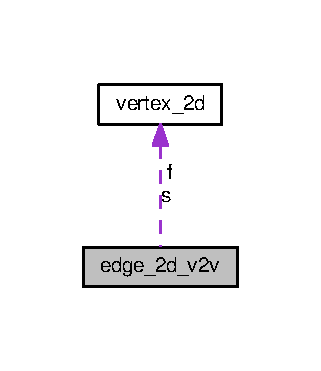
\includegraphics[width=154pt]{classedge__2d__v2v__coll__graph}
\end{center}
\end{figure}
\subsection*{Public Member Functions}
\begin{DoxyCompactItemize}
\item 
\hyperlink{classedge__2d__v2v_a47d30867a13efb336c942cb1a7d5703a}{edge\+\_\+2d\+\_\+v2v} (\hyperlink{classvertex__2d}{vertex\+\_\+2d} \hyperlink{classedge__2d__v2v_a329f701b47c323a9d200b62b208bf4c9}{f}, \hyperlink{classvertex__2d}{vertex\+\_\+2d} \hyperlink{classedge__2d__v2v_af2a0304bd993964329335adf6a574302}{s})
\begin{DoxyCompactList}\small\item\em Constructor. \end{DoxyCompactList}\end{DoxyCompactItemize}
\subsection*{Public Attributes}
\begin{DoxyCompactItemize}
\item 
\hyperlink{classvertex__2d}{vertex\+\_\+2d} \hyperlink{classedge__2d__v2v_a329f701b47c323a9d200b62b208bf4c9}{f}
\begin{DoxyCompactList}\small\item\em first end-\/point \end{DoxyCompactList}\item 
\hyperlink{classvertex__2d}{vertex\+\_\+2d} \hyperlink{classedge__2d__v2v_af2a0304bd993964329335adf6a574302}{s}
\begin{DoxyCompactList}\small\item\em second end-\/point \end{DoxyCompactList}\item 
bool \hyperlink{classedge__2d__v2v_a0d7a74be9d49be2c429b7274a3011119}{dash}
\begin{DoxyCompactList}\small\item\em boolean for if edge is dash or solid \end{DoxyCompactList}\end{DoxyCompactItemize}


\subsection{Detailed Description}
class for an \hyperlink{classedge__2d__v2v}{edge\+\_\+2d\+\_\+v2v} 

Definition at line 51 of file structs.\+h.



\subsection{Constructor \& Destructor Documentation}
\index{edge\+\_\+2d\+\_\+v2v@{edge\+\_\+2d\+\_\+v2v}!edge\+\_\+2d\+\_\+v2v@{edge\+\_\+2d\+\_\+v2v}}
\index{edge\+\_\+2d\+\_\+v2v@{edge\+\_\+2d\+\_\+v2v}!edge\+\_\+2d\+\_\+v2v@{edge\+\_\+2d\+\_\+v2v}}
\subsubsection[{\texorpdfstring{edge\+\_\+2d\+\_\+v2v(vertex\+\_\+2d f, vertex\+\_\+2d s)}{edge_2d_v2v(vertex_2d f, vertex_2d s)}}]{\setlength{\rightskip}{0pt plus 5cm}edge\+\_\+2d\+\_\+v2v\+::edge\+\_\+2d\+\_\+v2v (
\begin{DoxyParamCaption}
\item[{{\bf vertex\+\_\+2d}}]{f, }
\item[{{\bf vertex\+\_\+2d}}]{s}
\end{DoxyParamCaption}
)}\hypertarget{classedge__2d__v2v_a47d30867a13efb336c942cb1a7d5703a}{}\label{classedge__2d__v2v_a47d30867a13efb336c942cb1a7d5703a}


Constructor. 



Definition at line 41 of file structs.\+cpp.



\subsection{Member Data Documentation}
\index{edge\+\_\+2d\+\_\+v2v@{edge\+\_\+2d\+\_\+v2v}!dash@{dash}}
\index{dash@{dash}!edge\+\_\+2d\+\_\+v2v@{edge\+\_\+2d\+\_\+v2v}}
\subsubsection[{\texorpdfstring{dash}{dash}}]{\setlength{\rightskip}{0pt plus 5cm}bool edge\+\_\+2d\+\_\+v2v\+::dash}\hypertarget{classedge__2d__v2v_a0d7a74be9d49be2c429b7274a3011119}{}\label{classedge__2d__v2v_a0d7a74be9d49be2c429b7274a3011119}


boolean for if edge is dash or solid 



Definition at line 55 of file structs.\+h.

\index{edge\+\_\+2d\+\_\+v2v@{edge\+\_\+2d\+\_\+v2v}!f@{f}}
\index{f@{f}!edge\+\_\+2d\+\_\+v2v@{edge\+\_\+2d\+\_\+v2v}}
\subsubsection[{\texorpdfstring{f}{f}}]{\setlength{\rightskip}{0pt plus 5cm}{\bf vertex\+\_\+2d} edge\+\_\+2d\+\_\+v2v\+::f}\hypertarget{classedge__2d__v2v_a329f701b47c323a9d200b62b208bf4c9}{}\label{classedge__2d__v2v_a329f701b47c323a9d200b62b208bf4c9}


first end-\/point 



Definition at line 53 of file structs.\+h.

\index{edge\+\_\+2d\+\_\+v2v@{edge\+\_\+2d\+\_\+v2v}!s@{s}}
\index{s@{s}!edge\+\_\+2d\+\_\+v2v@{edge\+\_\+2d\+\_\+v2v}}
\subsubsection[{\texorpdfstring{s}{s}}]{\setlength{\rightskip}{0pt plus 5cm}{\bf vertex\+\_\+2d} edge\+\_\+2d\+\_\+v2v\+::s}\hypertarget{classedge__2d__v2v_af2a0304bd993964329335adf6a574302}{}\label{classedge__2d__v2v_af2a0304bd993964329335adf6a574302}


second end-\/point 



Definition at line 54 of file structs.\+h.



The documentation for this class was generated from the following files\+:\begin{DoxyCompactItemize}
\item 
\hyperlink{structs_8h}{structs.\+h}\item 
/home/manish/\+Desktop/\+Manish\+\_\+\+C\+A\+D\+\_\+\+Tool/src/\hyperlink{structs_8cpp}{structs.\+cpp}\end{DoxyCompactItemize}

\hypertarget{classedge__3d}{}\section{edge\+\_\+3d Class Reference}
\label{classedge__3d}\index{edge\+\_\+3d@{edge\+\_\+3d}}


class for an \hyperlink{classedge__3d}{edge\+\_\+3d}  




{\ttfamily \#include $<$structs.\+h$>$}

\subsection*{Public Member Functions}
\begin{DoxyCompactItemize}
\item 
\hyperlink{classedge__3d_afac87fcbf6f852908b7113dc2efe59d9}{edge\+\_\+3d} (int \hyperlink{classedge__3d_a1365e6035d117feb008f996290507425}{f}, int \hyperlink{classedge__3d_aa33edd90f3962b3caf4dd8780d3fd9fb}{s})
\begin{DoxyCompactList}\small\item\em Constructor. \end{DoxyCompactList}\item 
bool \hyperlink{classedge__3d_ac01ef82b4f0003f7b1bc84f47ac89e9c}{operator==} (const \hyperlink{classedge__3d}{edge\+\_\+3d} \&rhs)
\begin{DoxyCompactList}\small\item\em bool operator == for \hyperlink{classedge__3d}{edge\+\_\+3d} \end{DoxyCompactList}\end{DoxyCompactItemize}
\subsection*{Public Attributes}
\begin{DoxyCompactItemize}
\item 
int \hyperlink{classedge__3d_a1365e6035d117feb008f996290507425}{f}
\begin{DoxyCompactList}\small\item\em position of first end-\/point of the edge in v\+\_\+list \end{DoxyCompactList}\item 
int \hyperlink{classedge__3d_aa33edd90f3962b3caf4dd8780d3fd9fb}{s}
\begin{DoxyCompactList}\small\item\em position of second end-\/point of the edge in v\+\_\+list \end{DoxyCompactList}\end{DoxyCompactItemize}


\subsection{Detailed Description}
class for an \hyperlink{classedge__3d}{edge\+\_\+3d} 

Definition at line 97 of file structs.\+h.



\subsection{Constructor \& Destructor Documentation}
\index{edge\+\_\+3d@{edge\+\_\+3d}!edge\+\_\+3d@{edge\+\_\+3d}}
\index{edge\+\_\+3d@{edge\+\_\+3d}!edge\+\_\+3d@{edge\+\_\+3d}}
\subsubsection[{\texorpdfstring{edge\+\_\+3d(int f, int s)}{edge_3d(int f, int s)}}]{\setlength{\rightskip}{0pt plus 5cm}edge\+\_\+3d\+::edge\+\_\+3d (
\begin{DoxyParamCaption}
\item[{int}]{f, }
\item[{int}]{s}
\end{DoxyParamCaption}
)}\hypertarget{classedge__3d_afac87fcbf6f852908b7113dc2efe59d9}{}\label{classedge__3d_afac87fcbf6f852908b7113dc2efe59d9}


Constructor. 



Definition at line 89 of file structs.\+cpp.



\subsection{Member Function Documentation}
\index{edge\+\_\+3d@{edge\+\_\+3d}!operator==@{operator==}}
\index{operator==@{operator==}!edge\+\_\+3d@{edge\+\_\+3d}}
\subsubsection[{\texorpdfstring{operator==(const edge\+\_\+3d \&rhs)}{operator==(const edge_3d &rhs)}}]{\setlength{\rightskip}{0pt plus 5cm}bool edge\+\_\+3d\+::operator== (
\begin{DoxyParamCaption}
\item[{const {\bf edge\+\_\+3d} \&}]{rhs}
\end{DoxyParamCaption}
)}\hypertarget{classedge__3d_ac01ef82b4f0003f7b1bc84f47ac89e9c}{}\label{classedge__3d_ac01ef82b4f0003f7b1bc84f47ac89e9c}


bool operator == for \hyperlink{classedge__3d}{edge\+\_\+3d} 



Definition at line 94 of file structs.\+cpp.



\subsection{Member Data Documentation}
\index{edge\+\_\+3d@{edge\+\_\+3d}!f@{f}}
\index{f@{f}!edge\+\_\+3d@{edge\+\_\+3d}}
\subsubsection[{\texorpdfstring{f}{f}}]{\setlength{\rightskip}{0pt plus 5cm}int edge\+\_\+3d\+::f}\hypertarget{classedge__3d_a1365e6035d117feb008f996290507425}{}\label{classedge__3d_a1365e6035d117feb008f996290507425}


position of first end-\/point of the edge in v\+\_\+list 



Definition at line 99 of file structs.\+h.

\index{edge\+\_\+3d@{edge\+\_\+3d}!s@{s}}
\index{s@{s}!edge\+\_\+3d@{edge\+\_\+3d}}
\subsubsection[{\texorpdfstring{s}{s}}]{\setlength{\rightskip}{0pt plus 5cm}int edge\+\_\+3d\+::s}\hypertarget{classedge__3d_aa33edd90f3962b3caf4dd8780d3fd9fb}{}\label{classedge__3d_aa33edd90f3962b3caf4dd8780d3fd9fb}


position of second end-\/point of the edge in v\+\_\+list 



Definition at line 100 of file structs.\+h.



The documentation for this class was generated from the following files\+:\begin{DoxyCompactItemize}
\item 
\hyperlink{structs_8h}{structs.\+h}\item 
/home/manish/\+Desktop/\+Manish\+\_\+\+C\+A\+D\+\_\+\+Tool/src/\hyperlink{structs_8cpp}{structs.\+cpp}\end{DoxyCompactItemize}

\hypertarget{classface__loop}{}\section{face\+\_\+loop Class Reference}
\label{classface__loop}\index{face\+\_\+loop@{face\+\_\+loop}}


{\ttfamily \#include $<$faceloop\+\_\+generator.\+h$>$}



Collaboration diagram for face\+\_\+loop\+:
\nopagebreak
\begin{figure}[H]
\begin{center}
\leavevmode
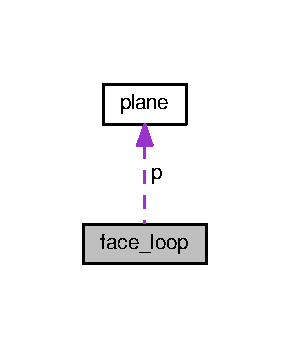
\includegraphics[width=139pt]{classface__loop__coll__graph}
\end{center}
\end{figure}
\subsection*{Public Member Functions}
\begin{DoxyCompactItemize}
\item 
\hyperlink{classface__loop_ad4fd127145cf380521f434dbc0d80828}{face\+\_\+loop} (std\+::vector$<$ \hyperlink{classbasic__loop}{basic\+\_\+loop} $>$ \hyperlink{classface__loop_a9eac12e0b3a21cd0dd5a6be0ad4f21c9}{basic\+\_\+loop\+\_\+list}, \hyperlink{classplane}{plane} \hyperlink{classface__loop_af184ff126eded4239b95693a8048c725}{p})
\begin{DoxyCompactList}\small\item\em Constructor. \end{DoxyCompactList}\item 
void \hyperlink{classface__loop_a52dba7a417fc35be60db0b120004c499}{add\+\_\+basic\+\_\+loop} (\hyperlink{classbasic__loop}{basic\+\_\+loop} bl)
\begin{DoxyCompactList}\small\item\em function that adds basic loop in the basic\+\_\+loop\+\_\+list \end{DoxyCompactList}\end{DoxyCompactItemize}
\subsection*{Public Attributes}
\begin{DoxyCompactItemize}
\item 
std\+::vector$<$ \hyperlink{classbasic__loop}{basic\+\_\+loop} $>$ \hyperlink{classface__loop_a9eac12e0b3a21cd0dd5a6be0ad4f21c9}{basic\+\_\+loop\+\_\+list}
\begin{DoxyCompactList}\small\item\em vector of \hyperlink{classbasic__loop}{basic\+\_\+loop} included in the faceloop \end{DoxyCompactList}\item 
\hyperlink{classplane}{plane} \hyperlink{classface__loop_af184ff126eded4239b95693a8048c725}{p}
\begin{DoxyCompactList}\small\item\em equation of plane on which faceloop is \end{DoxyCompactList}\end{DoxyCompactItemize}


\subsection{Detailed Description}


Definition at line 25 of file faceloop\+\_\+generator.\+h.



\subsection{Constructor \& Destructor Documentation}
\index{face\+\_\+loop@{face\+\_\+loop}!face\+\_\+loop@{face\+\_\+loop}}
\index{face\+\_\+loop@{face\+\_\+loop}!face\+\_\+loop@{face\+\_\+loop}}
\subsubsection[{\texorpdfstring{face\+\_\+loop(std\+::vector$<$ basic\+\_\+loop $>$ basic\+\_\+loop\+\_\+list, plane p)}{face_loop(std::vector< basic_loop > basic_loop_list, plane p)}}]{\setlength{\rightskip}{0pt plus 5cm}face\+\_\+loop\+::face\+\_\+loop (
\begin{DoxyParamCaption}
\item[{std\+::vector$<$ {\bf basic\+\_\+loop} $>$}]{basic\+\_\+loop\+\_\+list, }
\item[{{\bf plane}}]{p}
\end{DoxyParamCaption}
)}\hypertarget{classface__loop_ad4fd127145cf380521f434dbc0d80828}{}\label{classface__loop_ad4fd127145cf380521f434dbc0d80828}


Constructor. 



Definition at line 18 of file faceloop\+\_\+generator.\+cpp.



\subsection{Member Function Documentation}
\index{face\+\_\+loop@{face\+\_\+loop}!add\+\_\+basic\+\_\+loop@{add\+\_\+basic\+\_\+loop}}
\index{add\+\_\+basic\+\_\+loop@{add\+\_\+basic\+\_\+loop}!face\+\_\+loop@{face\+\_\+loop}}
\subsubsection[{\texorpdfstring{add\+\_\+basic\+\_\+loop(basic\+\_\+loop bl)}{add_basic_loop(basic_loop bl)}}]{\setlength{\rightskip}{0pt plus 5cm}void face\+\_\+loop\+::add\+\_\+basic\+\_\+loop (
\begin{DoxyParamCaption}
\item[{{\bf basic\+\_\+loop}}]{bl}
\end{DoxyParamCaption}
)}\hypertarget{classface__loop_a52dba7a417fc35be60db0b120004c499}{}\label{classface__loop_a52dba7a417fc35be60db0b120004c499}


function that adds basic loop in the basic\+\_\+loop\+\_\+list 



Definition at line 31 of file faceloop\+\_\+generator.\+cpp.



\subsection{Member Data Documentation}
\index{face\+\_\+loop@{face\+\_\+loop}!basic\+\_\+loop\+\_\+list@{basic\+\_\+loop\+\_\+list}}
\index{basic\+\_\+loop\+\_\+list@{basic\+\_\+loop\+\_\+list}!face\+\_\+loop@{face\+\_\+loop}}
\subsubsection[{\texorpdfstring{basic\+\_\+loop\+\_\+list}{basic_loop_list}}]{\setlength{\rightskip}{0pt plus 5cm}std\+::vector$<$ {\bf basic\+\_\+loop} $>$ face\+\_\+loop\+::basic\+\_\+loop\+\_\+list}\hypertarget{classface__loop_a9eac12e0b3a21cd0dd5a6be0ad4f21c9}{}\label{classface__loop_a9eac12e0b3a21cd0dd5a6be0ad4f21c9}


vector of \hyperlink{classbasic__loop}{basic\+\_\+loop} included in the faceloop 



Definition at line 29 of file faceloop\+\_\+generator.\+h.

\index{face\+\_\+loop@{face\+\_\+loop}!p@{p}}
\index{p@{p}!face\+\_\+loop@{face\+\_\+loop}}
\subsubsection[{\texorpdfstring{p}{p}}]{\setlength{\rightskip}{0pt plus 5cm}{\bf plane} face\+\_\+loop\+::p}\hypertarget{classface__loop_af184ff126eded4239b95693a8048c725}{}\label{classface__loop_af184ff126eded4239b95693a8048c725}


equation of plane on which faceloop is 



Definition at line 30 of file faceloop\+\_\+generator.\+h.



The documentation for this class was generated from the following files\+:\begin{DoxyCompactItemize}
\item 
\hyperlink{faceloop__generator_8h}{faceloop\+\_\+generator.\+h}\item 
/home/manish/\+Desktop/\+Manish\+\_\+\+C\+A\+D\+\_\+\+Tool/src/\hyperlink{faceloop__generator_8cpp}{faceloop\+\_\+generator.\+cpp}\end{DoxyCompactItemize}

\hypertarget{class_form}{}\section{Form Class Reference}
\label{class_form}\index{Form@{Form}}


{\ttfamily \#include $<$form.\+h$>$}



Inheritance diagram for Form\+:
\nopagebreak
\begin{figure}[H]
\begin{center}
\leavevmode
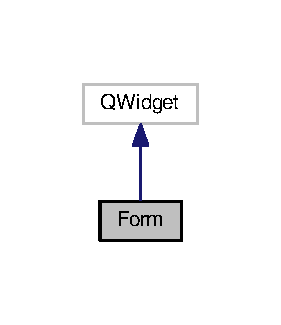
\includegraphics[width=135pt]{class_form__inherit__graph}
\end{center}
\end{figure}


Collaboration diagram for Form\+:
\nopagebreak
\begin{figure}[H]
\begin{center}
\leavevmode
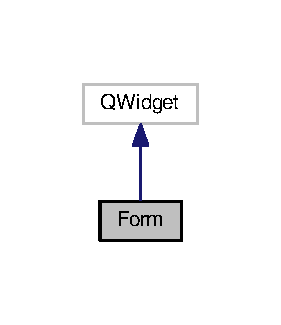
\includegraphics[width=135pt]{class_form__coll__graph}
\end{center}
\end{figure}
\subsection*{Public Member Functions}
\begin{DoxyCompactItemize}
\item 
\hyperlink{class_form_a9a921e26a02f23bffdea4330d6795796}{Form} (Q\+Widget $\ast$parent=0)
\item 
\hyperlink{class_form_a86c1cff1125ddd7abc626cc5b1f668af}{Form} (std\+::vector$<$ std\+::pair$<$ float, float $>$$>$ T, std\+::vector$<$ std\+::pair$<$ float, float $>$$>$ Fv, std\+::vector$<$ std\+::pair$<$ float, float $>$$>$ \hyperlink{form_8cpp_af933676109efed7ab34cea71d748a517}{S}, std\+::vector$<$ std\+::pair$<$ float, float $>$$>$ O, std\+::vector$<$ std\+::pair$<$ int, int $>$$>$ Te, std\+::vector$<$ std\+::pair$<$ int, int $>$$>$ Fe, std\+::vector$<$ std\+::pair$<$ int, int $>$$>$ Se, std\+::vector$<$ std\+::pair$<$ int, int $>$$>$ Oe, Q\+Widget $\ast$parent=0)
\item 
\hyperlink{class_form_a9cda7cce41e81bfaca51e922d4f9b98f}{$\sim$\+Form} ()
\end{DoxyCompactItemize}


\subsection{Detailed Description}


Definition at line 12 of file form.\+h.



\subsection{Constructor \& Destructor Documentation}
\index{Form@{Form}!Form@{Form}}
\index{Form@{Form}!Form@{Form}}
\subsubsection[{\texorpdfstring{Form(\+Q\+Widget $\ast$parent=0)}{Form(QWidget *parent=0)}}]{\setlength{\rightskip}{0pt plus 5cm}Form\+::\+Form (
\begin{DoxyParamCaption}
\item[{Q\+Widget $\ast$}]{parent = {\ttfamily 0}}
\end{DoxyParamCaption}
)\hspace{0.3cm}{\ttfamily [explicit]}}\hypertarget{class_form_a9a921e26a02f23bffdea4330d6795796}{}\label{class_form_a9a921e26a02f23bffdea4330d6795796}


Definition at line 23 of file form.\+cpp.

\index{Form@{Form}!Form@{Form}}
\index{Form@{Form}!Form@{Form}}
\subsubsection[{\texorpdfstring{Form(std\+::vector$<$ std\+::pair$<$ float, float $>$$>$ T, std\+::vector$<$ std\+::pair$<$ float, float $>$$>$ Fv, std\+::vector$<$ std\+::pair$<$ float, float $>$$>$ S, std\+::vector$<$ std\+::pair$<$ float, float $>$$>$ O, std\+::vector$<$ std\+::pair$<$ int, int $>$$>$ Te, std\+::vector$<$ std\+::pair$<$ int, int $>$$>$ Fe, std\+::vector$<$ std\+::pair$<$ int, int $>$$>$ Se, std\+::vector$<$ std\+::pair$<$ int, int $>$$>$ Oe, Q\+Widget $\ast$parent=0)}{Form(std::vector< std::pair< float, float >> T, std::vector< std::pair< float, float >> Fv, std::vector< std::pair< float, float >> S, std::vector< std::pair< float, float >> O, std::vector< std::pair< int, int >> Te, std::vector< std::pair< int, int >> Fe, std::vector< std::pair< int, int >> Se, std::vector< std::pair< int, int >> Oe, QWidget *parent=0)}}]{\setlength{\rightskip}{0pt plus 5cm}Form\+::\+Form (
\begin{DoxyParamCaption}
\item[{std\+::vector$<$ std\+::pair$<$ float, float $>$$>$}]{T, }
\item[{std\+::vector$<$ std\+::pair$<$ float, float $>$$>$}]{Fv, }
\item[{std\+::vector$<$ std\+::pair$<$ float, float $>$$>$}]{S, }
\item[{std\+::vector$<$ std\+::pair$<$ float, float $>$$>$}]{O, }
\item[{std\+::vector$<$ std\+::pair$<$ int, int $>$$>$}]{Te, }
\item[{std\+::vector$<$ std\+::pair$<$ int, int $>$$>$}]{Fe, }
\item[{std\+::vector$<$ std\+::pair$<$ int, int $>$$>$}]{Se, }
\item[{std\+::vector$<$ std\+::pair$<$ int, int $>$$>$}]{Oe, }
\item[{Q\+Widget $\ast$}]{parent = {\ttfamily 0}}
\end{DoxyParamCaption}
)}\hypertarget{class_form_a86c1cff1125ddd7abc626cc5b1f668af}{}\label{class_form_a86c1cff1125ddd7abc626cc5b1f668af}


Definition at line 29 of file form.\+cpp.

\index{Form@{Form}!````~Form@{$\sim$\+Form}}
\index{````~Form@{$\sim$\+Form}!Form@{Form}}
\subsubsection[{\texorpdfstring{$\sim$\+Form()}{~Form()}}]{\setlength{\rightskip}{0pt plus 5cm}Form\+::$\sim$\+Form (
\begin{DoxyParamCaption}
{}
\end{DoxyParamCaption}
)}\hypertarget{class_form_a9cda7cce41e81bfaca51e922d4f9b98f}{}\label{class_form_a9cda7cce41e81bfaca51e922d4f9b98f}


Definition at line 277 of file form.\+cpp.



The documentation for this class was generated from the following files\+:\begin{DoxyCompactItemize}
\item 
\hyperlink{form_8h}{form.\+h}\item 
/home/manish/\+Desktop/\+Manish\+\_\+\+C\+A\+D\+\_\+\+Tool/src/\hyperlink{form_8cpp}{form.\+cpp}\end{DoxyCompactItemize}

\hypertarget{class_full__plane}{}\section{Full\+\_\+plane Class Reference}
\label{class_full__plane}\index{Full\+\_\+plane@{Full\+\_\+plane}}


{\ttfamily \#include $<$Full\+\_\+plane.\+h$>$}



Collaboration diagram for Full\+\_\+plane\+:
\nopagebreak
\begin{figure}[H]
\begin{center}
\leavevmode
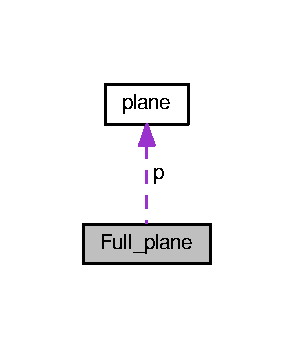
\includegraphics[width=141pt]{class_full__plane__coll__graph}
\end{center}
\end{figure}
\subsection*{Public Member Functions}
\begin{DoxyCompactItemize}
\item 
\hyperlink{class_full__plane_adc74c83d8c266176e717e54aff561a63}{Full\+\_\+plane} (\hyperlink{classplane}{plane} \hyperlink{class_full__plane_ad65bd61131d3c78d146592919a43fc3e}{p}, std\+::vector$<$ \hyperlink{classvertex__3d}{vertex\+\_\+3d} $>$ v3d\+\_\+list, std\+::vector$<$ \hyperlink{classedge__3d}{edge\+\_\+3d} $>$ e3d\+\_\+list)
\begin{DoxyCompactList}\small\item\em Constructor. \end{DoxyCompactList}\item 
\hyperlink{class_full__plane_a2dc5c95254d2537c62f6616418f53b6b}{Full\+\_\+plane} (\hyperlink{classplane}{plane} \hyperlink{class_full__plane_ad65bd61131d3c78d146592919a43fc3e}{p})
\begin{DoxyCompactList}\small\item\em Constructor. \end{DoxyCompactList}\item 
bool \hyperlink{class_full__plane_ad46ab0d796a3bfc10e7e8f4c2fa85bfc}{v\+\_\+on\+\_\+this\+\_\+plane} (\hyperlink{classvertex__3d}{vertex\+\_\+3d} v)
\begin{DoxyCompactList}\small\item\em function to check if the vertex v is on this plane or not \end{DoxyCompactList}\item 
bool \hyperlink{class_full__plane_a3bcb8b532890ad5b4abc7ed270b039de}{e\+\_\+on\+\_\+this\+\_\+plane} (\hyperlink{classvertex__3d}{vertex\+\_\+3d} v1, \hyperlink{classvertex__3d}{vertex\+\_\+3d} v2)
\begin{DoxyCompactList}\small\item\em function to check if the edge e is on this plane or not \end{DoxyCompactList}\item 
void \hyperlink{class_full__plane_a02b7ba0ae30cc09e077ac6d4b46a2db2}{add\+\_\+vertices} (std\+::vector$<$ \hyperlink{classvertex__3d}{vertex\+\_\+3d} $>$ v3d\+\_\+list)
\begin{DoxyCompactList}\small\item\em function to add the vertices which are on this plane \end{DoxyCompactList}\item 
void \hyperlink{class_full__plane_a155473c38443048865b1be6346cd011e}{add\+\_\+edges} (std\+::vector$<$ \hyperlink{classedge__3d}{edge\+\_\+3d} $>$ e3d\+\_\+list, std\+::vector$<$ \hyperlink{classvertex__3d}{vertex\+\_\+3d} $>$ v3d\+\_\+list)
\begin{DoxyCompactList}\small\item\em function to add the edges which are on this plane \end{DoxyCompactList}\end{DoxyCompactItemize}
\subsection*{Public Attributes}
\begin{DoxyCompactItemize}
\item 
\hyperlink{classplane}{plane} \hyperlink{class_full__plane_ad65bd61131d3c78d146592919a43fc3e}{p}
\begin{DoxyCompactList}\small\item\em equation of plane i.\+e (a,b,c,d) for ax + by + cz + d = 0 \end{DoxyCompactList}\item 
std\+::vector$<$ int $>$ \hyperlink{class_full__plane_a0b93d1b5a72f3fb83808edfce3bbcd1b}{vertices\+\_\+on\+\_\+it}
\begin{DoxyCompactList}\small\item\em vector of enum of vertices which are on this plane \end{DoxyCompactList}\item 
std\+::vector$<$ \hyperlink{classedge__3d}{edge\+\_\+3d} $>$ \hyperlink{class_full__plane_a88e6924e5ae6ef5ed92611ff849be290}{edges\+\_\+on\+\_\+it}
\begin{DoxyCompactList}\small\item\em vector of edges which are on this plane \end{DoxyCompactList}\end{DoxyCompactItemize}


\subsection{Detailed Description}


Definition at line 14 of file Full\+\_\+plane.\+h.



\subsection{Constructor \& Destructor Documentation}
\index{Full\+\_\+plane@{Full\+\_\+plane}!Full\+\_\+plane@{Full\+\_\+plane}}
\index{Full\+\_\+plane@{Full\+\_\+plane}!Full\+\_\+plane@{Full\+\_\+plane}}
\subsubsection[{\texorpdfstring{Full\+\_\+plane(plane p, std\+::vector$<$ vertex\+\_\+3d $>$ v3d\+\_\+list, std\+::vector$<$ edge\+\_\+3d $>$ e3d\+\_\+list)}{Full_plane(plane p, std::vector< vertex_3d > v3d_list, std::vector< edge_3d > e3d_list)}}]{\setlength{\rightskip}{0pt plus 5cm}Full\+\_\+plane\+::\+Full\+\_\+plane (
\begin{DoxyParamCaption}
\item[{{\bf plane}}]{p, }
\item[{std\+::vector$<$ {\bf vertex\+\_\+3d} $>$}]{v3d\+\_\+list, }
\item[{std\+::vector$<$ {\bf edge\+\_\+3d} $>$}]{e3d\+\_\+list}
\end{DoxyParamCaption}
)}\hypertarget{class_full__plane_adc74c83d8c266176e717e54aff561a63}{}\label{class_full__plane_adc74c83d8c266176e717e54aff561a63}


Constructor. 



Definition at line 7 of file Full\+\_\+plane.\+cpp.

\index{Full\+\_\+plane@{Full\+\_\+plane}!Full\+\_\+plane@{Full\+\_\+plane}}
\index{Full\+\_\+plane@{Full\+\_\+plane}!Full\+\_\+plane@{Full\+\_\+plane}}
\subsubsection[{\texorpdfstring{Full\+\_\+plane(plane p)}{Full_plane(plane p)}}]{\setlength{\rightskip}{0pt plus 5cm}Full\+\_\+plane\+::\+Full\+\_\+plane (
\begin{DoxyParamCaption}
\item[{{\bf plane}}]{p}
\end{DoxyParamCaption}
)}\hypertarget{class_full__plane_a2dc5c95254d2537c62f6616418f53b6b}{}\label{class_full__plane_a2dc5c95254d2537c62f6616418f53b6b}


Constructor. 



Definition at line 20 of file Full\+\_\+plane.\+cpp.



\subsection{Member Function Documentation}
\index{Full\+\_\+plane@{Full\+\_\+plane}!add\+\_\+edges@{add\+\_\+edges}}
\index{add\+\_\+edges@{add\+\_\+edges}!Full\+\_\+plane@{Full\+\_\+plane}}
\subsubsection[{\texorpdfstring{add\+\_\+edges(std\+::vector$<$ edge\+\_\+3d $>$ e3d\+\_\+list, std\+::vector$<$ vertex\+\_\+3d $>$ v3d\+\_\+list)}{add_edges(std::vector< edge_3d > e3d_list, std::vector< vertex_3d > v3d_list)}}]{\setlength{\rightskip}{0pt plus 5cm}void Full\+\_\+plane\+::add\+\_\+edges (
\begin{DoxyParamCaption}
\item[{std\+::vector$<$ {\bf edge\+\_\+3d} $>$}]{e3d\+\_\+list, }
\item[{std\+::vector$<$ {\bf vertex\+\_\+3d} $>$}]{v3d\+\_\+list}
\end{DoxyParamCaption}
)}\hypertarget{class_full__plane_a155473c38443048865b1be6346cd011e}{}\label{class_full__plane_a155473c38443048865b1be6346cd011e}


function to add the edges which are on this plane 


\begin{DoxyParams}{Parameters}
{\em e\+\_\+list} & edge list of 3D object \\
\hline
\end{DoxyParams}


Definition at line 54 of file Full\+\_\+plane.\+cpp.

\index{Full\+\_\+plane@{Full\+\_\+plane}!add\+\_\+vertices@{add\+\_\+vertices}}
\index{add\+\_\+vertices@{add\+\_\+vertices}!Full\+\_\+plane@{Full\+\_\+plane}}
\subsubsection[{\texorpdfstring{add\+\_\+vertices(std\+::vector$<$ vertex\+\_\+3d $>$ v3d\+\_\+list)}{add_vertices(std::vector< vertex_3d > v3d_list)}}]{\setlength{\rightskip}{0pt plus 5cm}void Full\+\_\+plane\+::add\+\_\+vertices (
\begin{DoxyParamCaption}
\item[{std\+::vector$<$ {\bf vertex\+\_\+3d} $>$}]{v3d\+\_\+list}
\end{DoxyParamCaption}
)}\hypertarget{class_full__plane_a02b7ba0ae30cc09e077ac6d4b46a2db2}{}\label{class_full__plane_a02b7ba0ae30cc09e077ac6d4b46a2db2}


function to add the vertices which are on this plane 


\begin{DoxyParams}{Parameters}
{\em v\+\_\+list} & vertex list of 3D object \\
\hline
\end{DoxyParams}


Definition at line 44 of file Full\+\_\+plane.\+cpp.

\index{Full\+\_\+plane@{Full\+\_\+plane}!e\+\_\+on\+\_\+this\+\_\+plane@{e\+\_\+on\+\_\+this\+\_\+plane}}
\index{e\+\_\+on\+\_\+this\+\_\+plane@{e\+\_\+on\+\_\+this\+\_\+plane}!Full\+\_\+plane@{Full\+\_\+plane}}
\subsubsection[{\texorpdfstring{e\+\_\+on\+\_\+this\+\_\+plane(vertex\+\_\+3d v1, vertex\+\_\+3d v2)}{e_on_this_plane(vertex_3d v1, vertex_3d v2)}}]{\setlength{\rightskip}{0pt plus 5cm}bool Full\+\_\+plane\+::e\+\_\+on\+\_\+this\+\_\+plane (
\begin{DoxyParamCaption}
\item[{{\bf vertex\+\_\+3d}}]{v1, }
\item[{{\bf vertex\+\_\+3d}}]{v2}
\end{DoxyParamCaption}
)}\hypertarget{class_full__plane_a3bcb8b532890ad5b4abc7ed270b039de}{}\label{class_full__plane_a3bcb8b532890ad5b4abc7ed270b039de}


function to check if the edge e is on this plane or not 



Definition at line 37 of file Full\+\_\+plane.\+cpp.

\index{Full\+\_\+plane@{Full\+\_\+plane}!v\+\_\+on\+\_\+this\+\_\+plane@{v\+\_\+on\+\_\+this\+\_\+plane}}
\index{v\+\_\+on\+\_\+this\+\_\+plane@{v\+\_\+on\+\_\+this\+\_\+plane}!Full\+\_\+plane@{Full\+\_\+plane}}
\subsubsection[{\texorpdfstring{v\+\_\+on\+\_\+this\+\_\+plane(vertex\+\_\+3d v)}{v_on_this_plane(vertex_3d v)}}]{\setlength{\rightskip}{0pt plus 5cm}bool Full\+\_\+plane\+::v\+\_\+on\+\_\+this\+\_\+plane (
\begin{DoxyParamCaption}
\item[{{\bf vertex\+\_\+3d}}]{v}
\end{DoxyParamCaption}
)}\hypertarget{class_full__plane_ad46ab0d796a3bfc10e7e8f4c2fa85bfc}{}\label{class_full__plane_ad46ab0d796a3bfc10e7e8f4c2fa85bfc}


function to check if the vertex v is on this plane or not 



Definition at line 27 of file Full\+\_\+plane.\+cpp.



\subsection{Member Data Documentation}
\index{Full\+\_\+plane@{Full\+\_\+plane}!edges\+\_\+on\+\_\+it@{edges\+\_\+on\+\_\+it}}
\index{edges\+\_\+on\+\_\+it@{edges\+\_\+on\+\_\+it}!Full\+\_\+plane@{Full\+\_\+plane}}
\subsubsection[{\texorpdfstring{edges\+\_\+on\+\_\+it}{edges_on_it}}]{\setlength{\rightskip}{0pt plus 5cm}std\+::vector$<${\bf edge\+\_\+3d}$>$ Full\+\_\+plane\+::edges\+\_\+on\+\_\+it}\hypertarget{class_full__plane_a88e6924e5ae6ef5ed92611ff849be290}{}\label{class_full__plane_a88e6924e5ae6ef5ed92611ff849be290}


vector of edges which are on this plane 



Definition at line 20 of file Full\+\_\+plane.\+h.

\index{Full\+\_\+plane@{Full\+\_\+plane}!p@{p}}
\index{p@{p}!Full\+\_\+plane@{Full\+\_\+plane}}
\subsubsection[{\texorpdfstring{p}{p}}]{\setlength{\rightskip}{0pt plus 5cm}{\bf plane} Full\+\_\+plane\+::p}\hypertarget{class_full__plane_ad65bd61131d3c78d146592919a43fc3e}{}\label{class_full__plane_ad65bd61131d3c78d146592919a43fc3e}


equation of plane i.\+e (a,b,c,d) for ax + by + cz + d = 0 



Definition at line 16 of file Full\+\_\+plane.\+h.

\index{Full\+\_\+plane@{Full\+\_\+plane}!vertices\+\_\+on\+\_\+it@{vertices\+\_\+on\+\_\+it}}
\index{vertices\+\_\+on\+\_\+it@{vertices\+\_\+on\+\_\+it}!Full\+\_\+plane@{Full\+\_\+plane}}
\subsubsection[{\texorpdfstring{vertices\+\_\+on\+\_\+it}{vertices_on_it}}]{\setlength{\rightskip}{0pt plus 5cm}std\+::vector$<$int$>$ Full\+\_\+plane\+::vertices\+\_\+on\+\_\+it}\hypertarget{class_full__plane_a0b93d1b5a72f3fb83808edfce3bbcd1b}{}\label{class_full__plane_a0b93d1b5a72f3fb83808edfce3bbcd1b}


vector of enum of vertices which are on this plane 



Definition at line 18 of file Full\+\_\+plane.\+h.



The documentation for this class was generated from the following files\+:\begin{DoxyCompactItemize}
\item 
\hyperlink{_full__plane_8h}{Full\+\_\+plane.\+h}\item 
/home/manish/\+Desktop/\+Manish\+\_\+\+C\+A\+D\+\_\+\+Tool/src/\hyperlink{_full__plane_8cpp}{Full\+\_\+plane.\+cpp}\end{DoxyCompactItemize}

\hypertarget{class_main_window}{}\section{Main\+Window Class Reference}
\label{class_main_window}\index{Main\+Window@{Main\+Window}}


{\ttfamily \#include $<$mainwindow.\+h$>$}



Inheritance diagram for Main\+Window\+:
\nopagebreak
\begin{figure}[H]
\begin{center}
\leavevmode
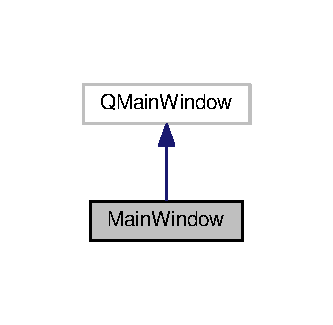
\includegraphics[width=160pt]{class_main_window__inherit__graph}
\end{center}
\end{figure}


Collaboration diagram for Main\+Window\+:
\nopagebreak
\begin{figure}[H]
\begin{center}
\leavevmode
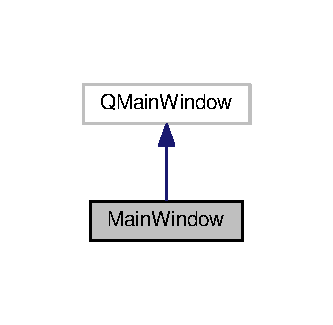
\includegraphics[width=160pt]{class_main_window__coll__graph}
\end{center}
\end{figure}
\subsection*{Public Member Functions}
\begin{DoxyCompactItemize}
\item 
\hyperlink{class_main_window_a8b244be8b7b7db1b08de2a2acb9409db}{Main\+Window} (Q\+Widget $\ast$parent=0)
\item 
\hyperlink{class_main_window_ae98d00a93bc118200eeef9f9bba1dba7}{$\sim$\+Main\+Window} ()
\end{DoxyCompactItemize}


\subsection{Detailed Description}


Definition at line 12 of file mainwindow.\+h.



\subsection{Constructor \& Destructor Documentation}
\index{Main\+Window@{Main\+Window}!Main\+Window@{Main\+Window}}
\index{Main\+Window@{Main\+Window}!Main\+Window@{Main\+Window}}
\subsubsection[{\texorpdfstring{Main\+Window(\+Q\+Widget $\ast$parent=0)}{MainWindow(QWidget *parent=0)}}]{\setlength{\rightskip}{0pt plus 5cm}Main\+Window\+::\+Main\+Window (
\begin{DoxyParamCaption}
\item[{Q\+Widget $\ast$}]{parent = {\ttfamily 0}}
\end{DoxyParamCaption}
)\hspace{0.3cm}{\ttfamily [explicit]}}\hypertarget{class_main_window_a8b244be8b7b7db1b08de2a2acb9409db}{}\label{class_main_window_a8b244be8b7b7db1b08de2a2acb9409db}


Definition at line 12 of file mainwindow.\+cpp.

\index{Main\+Window@{Main\+Window}!````~Main\+Window@{$\sim$\+Main\+Window}}
\index{````~Main\+Window@{$\sim$\+Main\+Window}!Main\+Window@{Main\+Window}}
\subsubsection[{\texorpdfstring{$\sim$\+Main\+Window()}{~MainWindow()}}]{\setlength{\rightskip}{0pt plus 5cm}Main\+Window\+::$\sim$\+Main\+Window (
\begin{DoxyParamCaption}
{}
\end{DoxyParamCaption}
)}\hypertarget{class_main_window_ae98d00a93bc118200eeef9f9bba1dba7}{}\label{class_main_window_ae98d00a93bc118200eeef9f9bba1dba7}


Definition at line 19 of file mainwindow.\+cpp.



The documentation for this class was generated from the following files\+:\begin{DoxyCompactItemize}
\item 
\hyperlink{mainwindow_8h}{mainwindow.\+h}\item 
/home/manish/\+Desktop/\+Manish\+\_\+\+C\+A\+D\+\_\+\+Tool/src/\hyperlink{mainwindow_8cpp}{mainwindow.\+cpp}\end{DoxyCompactItemize}

\hypertarget{class_object3d}{}\section{Object3d Class Reference}
\label{class_object3d}\index{Object3d@{Object3d}}


class for representation of a 3D object  




{\ttfamily \#include $<$Object\+\_\+3d.\+h$>$}



\subsection{Detailed Description}
class for representation of a 3D object 

The documentation for this class was generated from the following file\+:\begin{DoxyCompactItemize}
\item 
\hyperlink{_object__3d_8h}{Object\+\_\+3d.\+h}\end{DoxyCompactItemize}

\hypertarget{classobject__2d}{}\section{object\+\_\+2d Class Reference}
\label{classobject__2d}\index{object\+\_\+2d@{object\+\_\+2d}}


representation of \hyperlink{classobject__2d}{object\+\_\+2d}  




{\ttfamily \#include $<$object\+\_\+2d.\+h$>$}

\subsection*{Public Member Functions}
\begin{DoxyCompactItemize}
\item 
\hyperlink{classobject__2d_a3ed4eb36446c5dacac7cd84a3f73ba1f}{object\+\_\+2d} (std\+::vector$<$ \hyperlink{classvertex__2d}{vertex\+\_\+2d} $>$ \hyperlink{classobject__2d_aedcad81ef4cdb308ffade7bcf7de4cc2}{T\+\_\+vertices}, std\+::vector$<$ \hyperlink{classvertex__2d}{vertex\+\_\+2d} $>$ \hyperlink{classobject__2d_aa12b4ac9f646748a83b22c7a81ff1b7c}{F\+\_\+vertices}, std\+::vector$<$ \hyperlink{classvertex__2d}{vertex\+\_\+2d} $>$ \hyperlink{classobject__2d_a722b0505e408b8864809a7ae55c86df4}{S\+\_\+vertices}, std\+::vector$<$ \hyperlink{classedge__2d__v2v}{edge\+\_\+2d\+\_\+v2v} $>$ \hyperlink{classobject__2d_a1543063eb017187a7582821d1ec07faf}{T\+\_\+edges}, std\+::vector$<$ \hyperlink{classedge__2d__v2v}{edge\+\_\+2d\+\_\+v2v} $>$ \hyperlink{classobject__2d_abb23f1e7a00cef6deba5d997ff40a751}{F\+\_\+edges}, std\+::vector$<$ \hyperlink{classedge__2d__v2v}{edge\+\_\+2d\+\_\+v2v} $>$ \hyperlink{classobject__2d_ad13cc39539ebc9c5634ae59dea81e33c}{S\+\_\+edges})
\begin{DoxyCompactList}\small\item\em Constructor. \end{DoxyCompactList}\item 
\hyperlink{classobject__2d_a52104b7df912451e4dfdafeb2db8528f}{object\+\_\+2d} (std\+::vector$<$ \hyperlink{classvertex__3d}{vertex\+\_\+3d} $>$ v3d\+\_\+list, std\+::vector$<$ \hyperlink{classedge__3d}{edge\+\_\+3d} $>$ e3d\+\_\+list, std\+::vector$<$ std\+::vector$<$ \hyperlink{classedge__3d}{edge\+\_\+3d} $>$ $>$ surface\+\_\+list)
\item 
void \hyperlink{classobject__2d_a900bb547b93a4c92f3daf3acaf580333}{add\+\_\+\+T\+\_\+vertex} (\hyperlink{classvertex__2d}{vertex\+\_\+2d} v)
\begin{DoxyCompactList}\small\item\em function to add a vertex in the vector of vertices of Top-\/view \end{DoxyCompactList}\item 
void \hyperlink{classobject__2d_af46c50b2bcb0fd9188b35b818c960e8d}{add\+\_\+\+F\+\_\+vertex} (\hyperlink{classvertex__2d}{vertex\+\_\+2d} v)
\begin{DoxyCompactList}\small\item\em function to add a vertex in the vector of vertices of Front-\/view \end{DoxyCompactList}\item 
void \hyperlink{classobject__2d_a49f8d6d9a110979ac19eb40817d4d0ca}{add\+\_\+\+S\+\_\+vertex} (\hyperlink{classvertex__2d}{vertex\+\_\+2d} v)
\begin{DoxyCompactList}\small\item\em function to add a vertex in the vector of vertices of Side-\/view \end{DoxyCompactList}\item 
void \hyperlink{classobject__2d_adfe9c8ca6c38cf14338c1e37bb4fcc1f}{add\+\_\+\+T\+\_\+edge} (\hyperlink{classedge__2d}{edge\+\_\+2d} e)
\begin{DoxyCompactList}\small\item\em function to add an edge in the vector of edges of Top-\/view \end{DoxyCompactList}\item 
void \hyperlink{classobject__2d_ac6449512672c0ff45ca163c374b85466}{add\+\_\+\+F\+\_\+edge} (\hyperlink{classedge__2d}{edge\+\_\+2d} e)
\begin{DoxyCompactList}\small\item\em function to add an edge in the vector of edges of Front-\/view \end{DoxyCompactList}\item 
void \hyperlink{classobject__2d_a85c014c6fbb2c21ef42a06711dd0a277}{add\+\_\+\+S\+\_\+edge} (\hyperlink{classedge__2d}{edge\+\_\+2d} e)
\begin{DoxyCompactList}\small\item\em function to add an edge in the vector of edges of Side-\/view \end{DoxyCompactList}\item 
std\+::vector$<$ \hyperlink{classvertex__2d}{vertex\+\_\+2d} $>$ \hyperlink{classobject__2d_a68a06e7feae6a6cae1803f54b8a3a07b}{converter} (\hyperlink{classvertex__3d}{vertex\+\_\+3d} v)
\begin{DoxyCompactList}\small\item\em function to convert 3D vertex to 2D vertex and returns in the form of (v\+\_\+T,v\+\_\+F,v\+\_\+S) \end{DoxyCompactList}\item 
std\+::vector$<$ bool $>$ \hyperlink{classobject__2d_a7c2ffd764cf62444bdffdda7abef652c}{checker} (\hyperlink{classedge__3d}{edge\+\_\+3d} e)
\begin{DoxyCompactList}\small\item\em function to check that an edge in 3D is also an edge in top ,front and side views \end{DoxyCompactList}\end{DoxyCompactItemize}
\subsection*{Public Attributes}
\begin{DoxyCompactItemize}
\item 
std\+::vector$<$ \hyperlink{classvertex__2d}{vertex\+\_\+2d} $>$ \hyperlink{classobject__2d_aedcad81ef4cdb308ffade7bcf7de4cc2}{T\+\_\+vertices}
\begin{DoxyCompactList}\small\item\em vector of co-\/ordinates of vertices in top-\/view \end{DoxyCompactList}\item 
std\+::vector$<$ \hyperlink{classvertex__2d}{vertex\+\_\+2d} $>$ \hyperlink{classobject__2d_aa12b4ac9f646748a83b22c7a81ff1b7c}{F\+\_\+vertices}
\begin{DoxyCompactList}\small\item\em vector of co-\/ordinates of vertices in front-\/view \end{DoxyCompactList}\item 
std\+::vector$<$ \hyperlink{classvertex__2d}{vertex\+\_\+2d} $>$ \hyperlink{classobject__2d_a722b0505e408b8864809a7ae55c86df4}{S\+\_\+vertices}
\begin{DoxyCompactList}\small\item\em vector of co-\/ordinates of vertices in side-\/view \end{DoxyCompactList}\item 
std\+::vector$<$ \hyperlink{classedge__2d}{edge\+\_\+2d} $>$ \hyperlink{classobject__2d_a1543063eb017187a7582821d1ec07faf}{T\+\_\+edges}
\begin{DoxyCompactList}\small\item\em vector of edges in top-\/view \end{DoxyCompactList}\item 
std\+::vector$<$ \hyperlink{classedge__2d}{edge\+\_\+2d} $>$ \hyperlink{classobject__2d_abb23f1e7a00cef6deba5d997ff40a751}{F\+\_\+edges}
\begin{DoxyCompactList}\small\item\em vector of edges in front-\/view \end{DoxyCompactList}\item 
std\+::vector$<$ \hyperlink{classedge__2d}{edge\+\_\+2d} $>$ \hyperlink{classobject__2d_ad13cc39539ebc9c5634ae59dea81e33c}{S\+\_\+edges}
\begin{DoxyCompactList}\small\item\em vector of edges in side-\/view \end{DoxyCompactList}\end{DoxyCompactItemize}


\subsection{Detailed Description}
representation of \hyperlink{classobject__2d}{object\+\_\+2d} 

Definition at line 11 of file object\+\_\+2d.\+h.



\subsection{Constructor \& Destructor Documentation}
\index{object\+\_\+2d@{object\+\_\+2d}!object\+\_\+2d@{object\+\_\+2d}}
\index{object\+\_\+2d@{object\+\_\+2d}!object\+\_\+2d@{object\+\_\+2d}}
\subsubsection[{\texorpdfstring{object\+\_\+2d(std\+::vector$<$ vertex\+\_\+2d $>$ T\+\_\+vertices, std\+::vector$<$ vertex\+\_\+2d $>$ F\+\_\+vertices, std\+::vector$<$ vertex\+\_\+2d $>$ S\+\_\+vertices, std\+::vector$<$ edge\+\_\+2d\+\_\+v2v $>$ T\+\_\+edges, std\+::vector$<$ edge\+\_\+2d\+\_\+v2v $>$ F\+\_\+edges, std\+::vector$<$ edge\+\_\+2d\+\_\+v2v $>$ S\+\_\+edges)}{object_2d(std::vector< vertex_2d > T_vertices, std::vector< vertex_2d > F_vertices, std::vector< vertex_2d > S_vertices, std::vector< edge_2d_v2v > T_edges, std::vector< edge_2d_v2v > F_edges, std::vector< edge_2d_v2v > S_edges)}}]{\setlength{\rightskip}{0pt plus 5cm}object\+\_\+2d\+::object\+\_\+2d (
\begin{DoxyParamCaption}
\item[{std\+::vector$<$ {\bf vertex\+\_\+2d} $>$}]{T\+\_\+vertices, }
\item[{std\+::vector$<$ {\bf vertex\+\_\+2d} $>$}]{F\+\_\+vertices, }
\item[{std\+::vector$<$ {\bf vertex\+\_\+2d} $>$}]{S\+\_\+vertices, }
\item[{std\+::vector$<$ {\bf edge\+\_\+2d\+\_\+v2v} $>$}]{T\+\_\+edges, }
\item[{std\+::vector$<$ {\bf edge\+\_\+2d\+\_\+v2v} $>$}]{F\+\_\+edges, }
\item[{std\+::vector$<$ {\bf edge\+\_\+2d\+\_\+v2v} $>$}]{S\+\_\+edges}
\end{DoxyParamCaption}
)}\hypertarget{classobject__2d_a3ed4eb36446c5dacac7cd84a3f73ba1f}{}\label{classobject__2d_a3ed4eb36446c5dacac7cd84a3f73ba1f}


Constructor. 



Definition at line 6 of file object\+\_\+2d.\+cpp.

\index{object\+\_\+2d@{object\+\_\+2d}!object\+\_\+2d@{object\+\_\+2d}}
\index{object\+\_\+2d@{object\+\_\+2d}!object\+\_\+2d@{object\+\_\+2d}}
\subsubsection[{\texorpdfstring{object\+\_\+2d(std\+::vector$<$ vertex\+\_\+3d $>$ v3d\+\_\+list, std\+::vector$<$ edge\+\_\+3d $>$ e3d\+\_\+list, std\+::vector$<$ std\+::vector$<$ edge\+\_\+3d $>$ $>$ surface\+\_\+list)}{object_2d(std::vector< vertex_3d > v3d_list, std::vector< edge_3d > e3d_list, std::vector< std::vector< edge_3d > > surface_list)}}]{\setlength{\rightskip}{0pt plus 5cm}object\+\_\+2d\+::object\+\_\+2d (
\begin{DoxyParamCaption}
\item[{std\+::vector$<$ {\bf vertex\+\_\+3d} $>$}]{v3d\+\_\+list, }
\item[{std\+::vector$<$ {\bf edge\+\_\+3d} $>$}]{e3d\+\_\+list, }
\item[{std\+::vector$<$ std\+::vector$<$ {\bf edge\+\_\+3d} $>$ $>$}]{surface\+\_\+list}
\end{DoxyParamCaption}
)}\hypertarget{classobject__2d_a52104b7df912451e4dfdafeb2db8528f}{}\label{classobject__2d_a52104b7df912451e4dfdafeb2db8528f}
This constructor consists -\/
\begin{DoxyEnumerate}
\item Converting the 3D vertex into its projected vertex
\item Adding the obtained projected vertex in top, front and side vertex list
\item There should not be an edge between overlapping points
\item Adding edges to the front, top and side edge list if it is an egde in the solid
\item On the basis of checker result edge is added in the edgelist of 2D object 
\end{DoxyEnumerate}

Definition at line 94 of file object\+\_\+2d.\+cpp.



\subsection{Member Function Documentation}
\index{object\+\_\+2d@{object\+\_\+2d}!add\+\_\+\+F\+\_\+edge@{add\+\_\+\+F\+\_\+edge}}
\index{add\+\_\+\+F\+\_\+edge@{add\+\_\+\+F\+\_\+edge}!object\+\_\+2d@{object\+\_\+2d}}
\subsubsection[{\texorpdfstring{add\+\_\+\+F\+\_\+edge(edge\+\_\+2d e)}{add_F_edge(edge_2d e)}}]{\setlength{\rightskip}{0pt plus 5cm}void object\+\_\+2d\+::add\+\_\+\+F\+\_\+edge (
\begin{DoxyParamCaption}
\item[{{\bf edge\+\_\+2d}}]{e}
\end{DoxyParamCaption}
)}\hypertarget{classobject__2d_ac6449512672c0ff45ca163c374b85466}{}\label{classobject__2d_ac6449512672c0ff45ca163c374b85466}


function to add an edge in the vector of edges of Front-\/view 



Definition at line 158 of file object\+\_\+2d.\+cpp.

\index{object\+\_\+2d@{object\+\_\+2d}!add\+\_\+\+F\+\_\+vertex@{add\+\_\+\+F\+\_\+vertex}}
\index{add\+\_\+\+F\+\_\+vertex@{add\+\_\+\+F\+\_\+vertex}!object\+\_\+2d@{object\+\_\+2d}}
\subsubsection[{\texorpdfstring{add\+\_\+\+F\+\_\+vertex(vertex\+\_\+2d v)}{add_F_vertex(vertex_2d v)}}]{\setlength{\rightskip}{0pt plus 5cm}void object\+\_\+2d\+::add\+\_\+\+F\+\_\+vertex (
\begin{DoxyParamCaption}
\item[{{\bf vertex\+\_\+2d}}]{v}
\end{DoxyParamCaption}
)}\hypertarget{classobject__2d_af46c50b2bcb0fd9188b35b818c960e8d}{}\label{classobject__2d_af46c50b2bcb0fd9188b35b818c960e8d}


function to add a vertex in the vector of vertices of Front-\/view 



Definition at line 140 of file object\+\_\+2d.\+cpp.

\index{object\+\_\+2d@{object\+\_\+2d}!add\+\_\+\+S\+\_\+edge@{add\+\_\+\+S\+\_\+edge}}
\index{add\+\_\+\+S\+\_\+edge@{add\+\_\+\+S\+\_\+edge}!object\+\_\+2d@{object\+\_\+2d}}
\subsubsection[{\texorpdfstring{add\+\_\+\+S\+\_\+edge(edge\+\_\+2d e)}{add_S_edge(edge_2d e)}}]{\setlength{\rightskip}{0pt plus 5cm}void object\+\_\+2d\+::add\+\_\+\+S\+\_\+edge (
\begin{DoxyParamCaption}
\item[{{\bf edge\+\_\+2d}}]{e}
\end{DoxyParamCaption}
)}\hypertarget{classobject__2d_a85c014c6fbb2c21ef42a06711dd0a277}{}\label{classobject__2d_a85c014c6fbb2c21ef42a06711dd0a277}


function to add an edge in the vector of edges of Side-\/view 



Definition at line 164 of file object\+\_\+2d.\+cpp.

\index{object\+\_\+2d@{object\+\_\+2d}!add\+\_\+\+S\+\_\+vertex@{add\+\_\+\+S\+\_\+vertex}}
\index{add\+\_\+\+S\+\_\+vertex@{add\+\_\+\+S\+\_\+vertex}!object\+\_\+2d@{object\+\_\+2d}}
\subsubsection[{\texorpdfstring{add\+\_\+\+S\+\_\+vertex(vertex\+\_\+2d v)}{add_S_vertex(vertex_2d v)}}]{\setlength{\rightskip}{0pt plus 5cm}void object\+\_\+2d\+::add\+\_\+\+S\+\_\+vertex (
\begin{DoxyParamCaption}
\item[{{\bf vertex\+\_\+2d}}]{v}
\end{DoxyParamCaption}
)}\hypertarget{classobject__2d_a49f8d6d9a110979ac19eb40817d4d0ca}{}\label{classobject__2d_a49f8d6d9a110979ac19eb40817d4d0ca}


function to add a vertex in the vector of vertices of Side-\/view 



Definition at line 146 of file object\+\_\+2d.\+cpp.

\index{object\+\_\+2d@{object\+\_\+2d}!add\+\_\+\+T\+\_\+edge@{add\+\_\+\+T\+\_\+edge}}
\index{add\+\_\+\+T\+\_\+edge@{add\+\_\+\+T\+\_\+edge}!object\+\_\+2d@{object\+\_\+2d}}
\subsubsection[{\texorpdfstring{add\+\_\+\+T\+\_\+edge(edge\+\_\+2d e)}{add_T_edge(edge_2d e)}}]{\setlength{\rightskip}{0pt plus 5cm}void object\+\_\+2d\+::add\+\_\+\+T\+\_\+edge (
\begin{DoxyParamCaption}
\item[{{\bf edge\+\_\+2d}}]{e}
\end{DoxyParamCaption}
)}\hypertarget{classobject__2d_adfe9c8ca6c38cf14338c1e37bb4fcc1f}{}\label{classobject__2d_adfe9c8ca6c38cf14338c1e37bb4fcc1f}


function to add an edge in the vector of edges of Top-\/view 



Definition at line 152 of file object\+\_\+2d.\+cpp.

\index{object\+\_\+2d@{object\+\_\+2d}!add\+\_\+\+T\+\_\+vertex@{add\+\_\+\+T\+\_\+vertex}}
\index{add\+\_\+\+T\+\_\+vertex@{add\+\_\+\+T\+\_\+vertex}!object\+\_\+2d@{object\+\_\+2d}}
\subsubsection[{\texorpdfstring{add\+\_\+\+T\+\_\+vertex(vertex\+\_\+2d v)}{add_T_vertex(vertex_2d v)}}]{\setlength{\rightskip}{0pt plus 5cm}void object\+\_\+2d\+::add\+\_\+\+T\+\_\+vertex (
\begin{DoxyParamCaption}
\item[{{\bf vertex\+\_\+2d}}]{v}
\end{DoxyParamCaption}
)}\hypertarget{classobject__2d_a900bb547b93a4c92f3daf3acaf580333}{}\label{classobject__2d_a900bb547b93a4c92f3daf3acaf580333}


function to add a vertex in the vector of vertices of Top-\/view 



Definition at line 134 of file object\+\_\+2d.\+cpp.

\index{object\+\_\+2d@{object\+\_\+2d}!checker@{checker}}
\index{checker@{checker}!object\+\_\+2d@{object\+\_\+2d}}
\subsubsection[{\texorpdfstring{checker(edge\+\_\+3d e)}{checker(edge_3d e)}}]{\setlength{\rightskip}{0pt plus 5cm}std\+::vector$<$ bool $>$ object\+\_\+2d\+::checker (
\begin{DoxyParamCaption}
\item[{{\bf edge\+\_\+3d}}]{e}
\end{DoxyParamCaption}
)}\hypertarget{classobject__2d_a7c2ffd764cf62444bdffdda7abef652c}{}\label{classobject__2d_a7c2ffd764cf62444bdffdda7abef652c}


function to check that an edge in 3D is also an edge in top ,front and side views 



Definition at line 195 of file object\+\_\+2d.\+cpp.

\index{object\+\_\+2d@{object\+\_\+2d}!converter@{converter}}
\index{converter@{converter}!object\+\_\+2d@{object\+\_\+2d}}
\subsubsection[{\texorpdfstring{converter(vertex\+\_\+3d v)}{converter(vertex_3d v)}}]{\setlength{\rightskip}{0pt plus 5cm}std\+::vector$<$ {\bf vertex\+\_\+2d} $>$ object\+\_\+2d\+::converter (
\begin{DoxyParamCaption}
\item[{{\bf vertex\+\_\+3d}}]{v}
\end{DoxyParamCaption}
)}\hypertarget{classobject__2d_a68a06e7feae6a6cae1803f54b8a3a07b}{}\label{classobject__2d_a68a06e7feae6a6cae1803f54b8a3a07b}


function to convert 3D vertex to 2D vertex and returns in the form of (v\+\_\+T,v\+\_\+F,v\+\_\+S) 



Definition at line 175 of file object\+\_\+2d.\+cpp.



\subsection{Member Data Documentation}
\index{object\+\_\+2d@{object\+\_\+2d}!F\+\_\+edges@{F\+\_\+edges}}
\index{F\+\_\+edges@{F\+\_\+edges}!object\+\_\+2d@{object\+\_\+2d}}
\subsubsection[{\texorpdfstring{F\+\_\+edges}{F_edges}}]{\setlength{\rightskip}{0pt plus 5cm}std\+::vector$<${\bf edge\+\_\+2d}$>$ object\+\_\+2d\+::\+F\+\_\+edges}\hypertarget{classobject__2d_abb23f1e7a00cef6deba5d997ff40a751}{}\label{classobject__2d_abb23f1e7a00cef6deba5d997ff40a751}


vector of edges in front-\/view 



Definition at line 18 of file object\+\_\+2d.\+h.

\index{object\+\_\+2d@{object\+\_\+2d}!F\+\_\+vertices@{F\+\_\+vertices}}
\index{F\+\_\+vertices@{F\+\_\+vertices}!object\+\_\+2d@{object\+\_\+2d}}
\subsubsection[{\texorpdfstring{F\+\_\+vertices}{F_vertices}}]{\setlength{\rightskip}{0pt plus 5cm}std\+::vector$<${\bf vertex\+\_\+2d}$>$ object\+\_\+2d\+::\+F\+\_\+vertices}\hypertarget{classobject__2d_aa12b4ac9f646748a83b22c7a81ff1b7c}{}\label{classobject__2d_aa12b4ac9f646748a83b22c7a81ff1b7c}


vector of co-\/ordinates of vertices in front-\/view 



Definition at line 15 of file object\+\_\+2d.\+h.

\index{object\+\_\+2d@{object\+\_\+2d}!S\+\_\+edges@{S\+\_\+edges}}
\index{S\+\_\+edges@{S\+\_\+edges}!object\+\_\+2d@{object\+\_\+2d}}
\subsubsection[{\texorpdfstring{S\+\_\+edges}{S_edges}}]{\setlength{\rightskip}{0pt plus 5cm}std\+::vector$<${\bf edge\+\_\+2d}$>$ object\+\_\+2d\+::\+S\+\_\+edges}\hypertarget{classobject__2d_ad13cc39539ebc9c5634ae59dea81e33c}{}\label{classobject__2d_ad13cc39539ebc9c5634ae59dea81e33c}


vector of edges in side-\/view 



Definition at line 19 of file object\+\_\+2d.\+h.

\index{object\+\_\+2d@{object\+\_\+2d}!S\+\_\+vertices@{S\+\_\+vertices}}
\index{S\+\_\+vertices@{S\+\_\+vertices}!object\+\_\+2d@{object\+\_\+2d}}
\subsubsection[{\texorpdfstring{S\+\_\+vertices}{S_vertices}}]{\setlength{\rightskip}{0pt plus 5cm}std\+::vector$<${\bf vertex\+\_\+2d}$>$ object\+\_\+2d\+::\+S\+\_\+vertices}\hypertarget{classobject__2d_a722b0505e408b8864809a7ae55c86df4}{}\label{classobject__2d_a722b0505e408b8864809a7ae55c86df4}


vector of co-\/ordinates of vertices in side-\/view 



Definition at line 16 of file object\+\_\+2d.\+h.

\index{object\+\_\+2d@{object\+\_\+2d}!T\+\_\+edges@{T\+\_\+edges}}
\index{T\+\_\+edges@{T\+\_\+edges}!object\+\_\+2d@{object\+\_\+2d}}
\subsubsection[{\texorpdfstring{T\+\_\+edges}{T_edges}}]{\setlength{\rightskip}{0pt plus 5cm}std\+::vector$<${\bf edge\+\_\+2d}$>$ object\+\_\+2d\+::\+T\+\_\+edges}\hypertarget{classobject__2d_a1543063eb017187a7582821d1ec07faf}{}\label{classobject__2d_a1543063eb017187a7582821d1ec07faf}


vector of edges in top-\/view 



Definition at line 17 of file object\+\_\+2d.\+h.

\index{object\+\_\+2d@{object\+\_\+2d}!T\+\_\+vertices@{T\+\_\+vertices}}
\index{T\+\_\+vertices@{T\+\_\+vertices}!object\+\_\+2d@{object\+\_\+2d}}
\subsubsection[{\texorpdfstring{T\+\_\+vertices}{T_vertices}}]{\setlength{\rightskip}{0pt plus 5cm}std\+::vector$<${\bf vertex\+\_\+2d}$>$ object\+\_\+2d\+::\+T\+\_\+vertices}\hypertarget{classobject__2d_aedcad81ef4cdb308ffade7bcf7de4cc2}{}\label{classobject__2d_aedcad81ef4cdb308ffade7bcf7de4cc2}


vector of co-\/ordinates of vertices in top-\/view 



Definition at line 14 of file object\+\_\+2d.\+h.



The documentation for this class was generated from the following files\+:\begin{DoxyCompactItemize}
\item 
\hyperlink{object__2d_8h}{object\+\_\+2d.\+h}\item 
/home/manish/\+Desktop/\+Manish\+\_\+\+C\+A\+D\+\_\+\+Tool/src/\hyperlink{object__2d_8cpp}{object\+\_\+2d.\+cpp}\end{DoxyCompactItemize}

\hypertarget{class_object__3d}{}\section{Object\+\_\+3d Class Reference}
\label{class_object__3d}\index{Object\+\_\+3d@{Object\+\_\+3d}}


{\ttfamily \#include $<$Object\+\_\+3d.\+h$>$}

\subsection*{Public Member Functions}
\begin{DoxyCompactItemize}
\item 
\hyperlink{class_object__3d_ad2e34d10075c342d690bd8d6648af371}{Object\+\_\+3d} (std\+::vector$<$ \hyperlink{classvertex__3d}{vertex\+\_\+3d} $>$ \hyperlink{class_object__3d_a7817c087a9d1bb4f0e077e2b070e9596}{v3d\+\_\+list}, std\+::vector$<$ \hyperlink{classedge__3d}{edge\+\_\+3d} $>$ \hyperlink{class_object__3d_a678f396b3aa4a3c0958ec0c7b7f36e89}{e3d\+\_\+list}, std\+::vector$<$ std\+::vector$<$ int $>$ $>$ \hyperlink{class_object__3d_a979ba92cf69caa653b89cf75fd278afe}{surface\+\_\+list})
\begin{DoxyCompactList}\small\item\em Constructor. \end{DoxyCompactList}\item 
\hyperlink{class_object__3d_abe30ddbc60c6bff11d4603ddfbd0e7c8}{Object\+\_\+3d} (\hyperlink{classobject__2d}{object\+\_\+2d} o)
\item 
\hyperlink{class_object__3d_aab341c1f81c8c3d18e7246c7bdc3ad27}{Object\+\_\+3d} ()
\item 
void \hyperlink{class_object__3d_a52e3ed72c9afd7e0cbe1191f0ae7be03}{add\+\_\+vertex} (\hyperlink{classvertex__3d}{vertex\+\_\+3d} v)
\begin{DoxyCompactList}\small\item\em function to add a vertex in the vector of vertices \end{DoxyCompactList}\item 
void \hyperlink{class_object__3d_a19b46c5f95adb7b81cf8ee514b6bef60}{add\+\_\+edge} (\hyperlink{classedge__3d}{edge\+\_\+3d} e)
\begin{DoxyCompactList}\small\item\em function to add an edge in the vector of edges \end{DoxyCompactList}\item 
void \hyperlink{class_object__3d_a546b0512f0df977d381ab4964ab12a9b}{remove\+\_\+edge} (\hyperlink{classedge__3d}{edge\+\_\+3d} e)
\begin{DoxyCompactList}\small\item\em function to remove an edge in the vector of edges \end{DoxyCompactList}\end{DoxyCompactItemize}
\subsection*{Public Attributes}
\begin{DoxyCompactItemize}
\item 
std\+::vector$<$ \hyperlink{classvertex__3d}{vertex\+\_\+3d} $>$ \hyperlink{class_object__3d_a7817c087a9d1bb4f0e077e2b070e9596}{v3d\+\_\+list}
\begin{DoxyCompactList}\small\item\em vector of 3d vertices \end{DoxyCompactList}\item 
std\+::vector$<$ \hyperlink{classedge__3d}{edge\+\_\+3d} $>$ \hyperlink{class_object__3d_a678f396b3aa4a3c0958ec0c7b7f36e89}{e3d\+\_\+list}
\begin{DoxyCompactList}\small\item\em vector of 3d edges \end{DoxyCompactList}\item 
std\+::vector$<$ std\+::vector$<$ int $>$ $>$ \hyperlink{class_object__3d_a979ba92cf69caa653b89cf75fd278afe}{surface\+\_\+list}
\end{DoxyCompactItemize}


\subsection{Detailed Description}


Definition at line 36 of file Object\+\_\+3d.\+h.



\subsection{Constructor \& Destructor Documentation}
\index{Object\+\_\+3d@{Object\+\_\+3d}!Object\+\_\+3d@{Object\+\_\+3d}}
\index{Object\+\_\+3d@{Object\+\_\+3d}!Object\+\_\+3d@{Object\+\_\+3d}}
\subsubsection[{\texorpdfstring{Object\+\_\+3d(std\+::vector$<$ vertex\+\_\+3d $>$ v3d\+\_\+list, std\+::vector$<$ edge\+\_\+3d $>$ e3d\+\_\+list, std\+::vector$<$ std\+::vector$<$ int $>$ $>$ surface\+\_\+list)}{Object_3d(std::vector< vertex_3d > v3d_list, std::vector< edge_3d > e3d_list, std::vector< std::vector< int > > surface_list)}}]{\setlength{\rightskip}{0pt plus 5cm}Object\+\_\+3d\+::\+Object\+\_\+3d (
\begin{DoxyParamCaption}
\item[{std\+::vector$<$ {\bf vertex\+\_\+3d} $>$}]{v3d\+\_\+list, }
\item[{std\+::vector$<$ {\bf edge\+\_\+3d} $>$}]{e3d\+\_\+list, }
\item[{std\+::vector$<$ std\+::vector$<$ int $>$ $>$}]{surface\+\_\+list}
\end{DoxyParamCaption}
)}\hypertarget{class_object__3d_ad2e34d10075c342d690bd8d6648af371}{}\label{class_object__3d_ad2e34d10075c342d690bd8d6648af371}


Constructor. 



Definition at line 13 of file Object\+\_\+3d.\+cpp.

\index{Object\+\_\+3d@{Object\+\_\+3d}!Object\+\_\+3d@{Object\+\_\+3d}}
\index{Object\+\_\+3d@{Object\+\_\+3d}!Object\+\_\+3d@{Object\+\_\+3d}}
\subsubsection[{\texorpdfstring{Object\+\_\+3d(object\+\_\+2d o)}{Object_3d(object_2d o)}}]{\setlength{\rightskip}{0pt plus 5cm}Object\+\_\+3d\+::\+Object\+\_\+3d (
\begin{DoxyParamCaption}
\item[{{\bf object\+\_\+2d}}]{o}
\end{DoxyParamCaption}
)}\hypertarget{class_object__3d_abe30ddbc60c6bff11d4603ddfbd0e7c8}{}\label{class_object__3d_abe30ddbc60c6bff11d4603ddfbd0e7c8}
This constructor consists -\/
\begin{DoxyEnumerate}
\item Adding vertices
\item Decision-\/tree processing for adding edges.
\item R\+ER (Redundant Edges Removal)
\item Planer graph generation
\item Face Loop generation
\item Body Part generation 
\end{DoxyEnumerate}

Definition at line 42 of file Object\+\_\+3d.\+cpp.

\index{Object\+\_\+3d@{Object\+\_\+3d}!Object\+\_\+3d@{Object\+\_\+3d}}
\index{Object\+\_\+3d@{Object\+\_\+3d}!Object\+\_\+3d@{Object\+\_\+3d}}
\subsubsection[{\texorpdfstring{Object\+\_\+3d()}{Object_3d()}}]{\setlength{\rightskip}{0pt plus 5cm}Object\+\_\+3d\+::\+Object\+\_\+3d (
\begin{DoxyParamCaption}
{}
\end{DoxyParamCaption}
)}\hypertarget{class_object__3d_aab341c1f81c8c3d18e7246c7bdc3ad27}{}\label{class_object__3d_aab341c1f81c8c3d18e7246c7bdc3ad27}


Definition at line 82 of file Object\+\_\+3d.\+cpp.



\subsection{Member Function Documentation}
\index{Object\+\_\+3d@{Object\+\_\+3d}!add\+\_\+edge@{add\+\_\+edge}}
\index{add\+\_\+edge@{add\+\_\+edge}!Object\+\_\+3d@{Object\+\_\+3d}}
\subsubsection[{\texorpdfstring{add\+\_\+edge(edge\+\_\+3d e)}{add_edge(edge_3d e)}}]{\setlength{\rightskip}{0pt plus 5cm}void Object\+\_\+3d\+::add\+\_\+edge (
\begin{DoxyParamCaption}
\item[{{\bf edge\+\_\+3d}}]{e}
\end{DoxyParamCaption}
)}\hypertarget{class_object__3d_a19b46c5f95adb7b81cf8ee514b6bef60}{}\label{class_object__3d_a19b46c5f95adb7b81cf8ee514b6bef60}


function to add an edge in the vector of edges 



Definition at line 94 of file Object\+\_\+3d.\+cpp.

\index{Object\+\_\+3d@{Object\+\_\+3d}!add\+\_\+vertex@{add\+\_\+vertex}}
\index{add\+\_\+vertex@{add\+\_\+vertex}!Object\+\_\+3d@{Object\+\_\+3d}}
\subsubsection[{\texorpdfstring{add\+\_\+vertex(vertex\+\_\+3d v)}{add_vertex(vertex_3d v)}}]{\setlength{\rightskip}{0pt plus 5cm}void Object\+\_\+3d\+::add\+\_\+vertex (
\begin{DoxyParamCaption}
\item[{{\bf vertex\+\_\+3d}}]{v}
\end{DoxyParamCaption}
)}\hypertarget{class_object__3d_a52e3ed72c9afd7e0cbe1191f0ae7be03}{}\label{class_object__3d_a52e3ed72c9afd7e0cbe1191f0ae7be03}


function to add a vertex in the vector of vertices 



Definition at line 89 of file Object\+\_\+3d.\+cpp.

\index{Object\+\_\+3d@{Object\+\_\+3d}!remove\+\_\+edge@{remove\+\_\+edge}}
\index{remove\+\_\+edge@{remove\+\_\+edge}!Object\+\_\+3d@{Object\+\_\+3d}}
\subsubsection[{\texorpdfstring{remove\+\_\+edge(edge\+\_\+3d e)}{remove_edge(edge_3d e)}}]{\setlength{\rightskip}{0pt plus 5cm}void Object\+\_\+3d\+::remove\+\_\+edge (
\begin{DoxyParamCaption}
\item[{{\bf edge\+\_\+3d}}]{e}
\end{DoxyParamCaption}
)}\hypertarget{class_object__3d_a546b0512f0df977d381ab4964ab12a9b}{}\label{class_object__3d_a546b0512f0df977d381ab4964ab12a9b}


function to remove an edge in the vector of edges 



Definition at line 99 of file Object\+\_\+3d.\+cpp.



\subsection{Member Data Documentation}
\index{Object\+\_\+3d@{Object\+\_\+3d}!e3d\+\_\+list@{e3d\+\_\+list}}
\index{e3d\+\_\+list@{e3d\+\_\+list}!Object\+\_\+3d@{Object\+\_\+3d}}
\subsubsection[{\texorpdfstring{e3d\+\_\+list}{e3d_list}}]{\setlength{\rightskip}{0pt plus 5cm}std\+::vector$<${\bf edge\+\_\+3d}$>$ Object\+\_\+3d\+::e3d\+\_\+list}\hypertarget{class_object__3d_a678f396b3aa4a3c0958ec0c7b7f36e89}{}\label{class_object__3d_a678f396b3aa4a3c0958ec0c7b7f36e89}


vector of 3d edges 



Definition at line 41 of file Object\+\_\+3d.\+h.

\index{Object\+\_\+3d@{Object\+\_\+3d}!surface\+\_\+list@{surface\+\_\+list}}
\index{surface\+\_\+list@{surface\+\_\+list}!Object\+\_\+3d@{Object\+\_\+3d}}
\subsubsection[{\texorpdfstring{surface\+\_\+list}{surface_list}}]{\setlength{\rightskip}{0pt plus 5cm}std\+::vector$<$ std\+::vector$<$int$>$ $>$ Object\+\_\+3d\+::surface\+\_\+list}\hypertarget{class_object__3d_a979ba92cf69caa653b89cf75fd278afe}{}\label{class_object__3d_a979ba92cf69caa653b89cf75fd278afe}
vector of surfaces, one surface is vector of 3d edges 

Definition at line 43 of file Object\+\_\+3d.\+h.

\index{Object\+\_\+3d@{Object\+\_\+3d}!v3d\+\_\+list@{v3d\+\_\+list}}
\index{v3d\+\_\+list@{v3d\+\_\+list}!Object\+\_\+3d@{Object\+\_\+3d}}
\subsubsection[{\texorpdfstring{v3d\+\_\+list}{v3d_list}}]{\setlength{\rightskip}{0pt plus 5cm}std\+::vector$<${\bf vertex\+\_\+3d}$>$ Object\+\_\+3d\+::v3d\+\_\+list}\hypertarget{class_object__3d_a7817c087a9d1bb4f0e077e2b070e9596}{}\label{class_object__3d_a7817c087a9d1bb4f0e077e2b070e9596}


vector of 3d vertices 



Definition at line 39 of file Object\+\_\+3d.\+h.



The documentation for this class was generated from the following files\+:\begin{DoxyCompactItemize}
\item 
\hyperlink{_object__3d_8h}{Object\+\_\+3d.\+h}\item 
/home/manish/\+Desktop/\+Manish\+\_\+\+C\+A\+D\+\_\+\+Tool/src/\hyperlink{_object__3d_8cpp}{Object\+\_\+3d.\+cpp}\end{DoxyCompactItemize}

\hypertarget{classplane}{}\section{plane Class Reference}
\label{classplane}\index{plane@{plane}}


class for a plane plane represented as (a,b,c,d) corresponding to the equation ax + by + cz = d  




{\ttfamily \#include $<$structs.\+h$>$}

\subsection*{Public Member Functions}
\begin{DoxyCompactItemize}
\item 
\hyperlink{classplane_adbf234bb1d3aca2d226e32cb6dea9199}{plane} (float \hyperlink{classplane_a93c319b577955eca012b2866db926c1f}{a}, float \hyperlink{classplane_af4a97d4328067448317dd787e048bc70}{b}, float \hyperlink{classplane_a3024e149a5b2cb4697fa71ae7d539bd1}{c}, float \hyperlink{classplane_a9a3cb65698785bad8199e7afbd083e27}{d})
\begin{DoxyCompactList}\small\item\em constructor for a plane \end{DoxyCompactList}\item 
\hyperlink{classplane_ab36174f444a88d3a53d9892828308b48}{plane} ()
\begin{DoxyCompactList}\small\item\em constructor for a plane \end{DoxyCompactList}\item 
void \hyperlink{classplane_ab58a90304cbd0db72264be65b3207677}{printit} ()
\begin{DoxyCompactList}\small\item\em print(); \end{DoxyCompactList}\end{DoxyCompactItemize}
\subsection*{Public Attributes}
\begin{DoxyCompactItemize}
\item 
float \hyperlink{classplane_a93c319b577955eca012b2866db926c1f}{a}
\item 
float \hyperlink{classplane_af4a97d4328067448317dd787e048bc70}{b}
\item 
float \hyperlink{classplane_a3024e149a5b2cb4697fa71ae7d539bd1}{c}
\item 
float \hyperlink{classplane_a9a3cb65698785bad8199e7afbd083e27}{d}
\end{DoxyCompactItemize}


\subsection{Detailed Description}
class for a plane plane represented as (a,b,c,d) corresponding to the equation ax + by + cz = d 

Definition at line 113 of file structs.\+h.



\subsection{Constructor \& Destructor Documentation}
\index{plane@{plane}!plane@{plane}}
\index{plane@{plane}!plane@{plane}}
\subsubsection[{\texorpdfstring{plane(float a, float b, float c, float d)}{plane(float a, float b, float c, float d)}}]{\setlength{\rightskip}{0pt plus 5cm}plane\+::plane (
\begin{DoxyParamCaption}
\item[{float}]{a, }
\item[{float}]{b, }
\item[{float}]{c, }
\item[{float}]{d}
\end{DoxyParamCaption}
)}\hypertarget{classplane_adbf234bb1d3aca2d226e32cb6dea9199}{}\label{classplane_adbf234bb1d3aca2d226e32cb6dea9199}


constructor for a plane 

This constructor edits (a,b,c,d) as following -\/ if d is non-\/zero (a\textquotesingle{},b\textquotesingle{},c\textquotesingle{},d\textquotesingle{}) = (a/d,b/d,c/d,1) else if c is non-\/zero (a\textquotesingle{},b\textquotesingle{},c\textquotesingle{},0) = (a/c,b/c,1,0) else if b is non-\/zero (a\textquotesingle{},b\textquotesingle{},0,0) = (a/b,1,0,0) else (a\textquotesingle{}0,0,0) = (1,0,0,0) 

Definition at line 109 of file structs.\+cpp.

\index{plane@{plane}!plane@{plane}}
\index{plane@{plane}!plane@{plane}}
\subsubsection[{\texorpdfstring{plane()}{plane()}}]{\setlength{\rightskip}{0pt plus 5cm}plane\+::plane (
\begin{DoxyParamCaption}
{}
\end{DoxyParamCaption}
)}\hypertarget{classplane_ab36174f444a88d3a53d9892828308b48}{}\label{classplane_ab36174f444a88d3a53d9892828308b48}


constructor for a plane 



Definition at line 99 of file structs.\+cpp.



\subsection{Member Function Documentation}
\index{plane@{plane}!printit@{printit}}
\index{printit@{printit}!plane@{plane}}
\subsubsection[{\texorpdfstring{printit()}{printit()}}]{\setlength{\rightskip}{0pt plus 5cm}void plane\+::printit (
\begin{DoxyParamCaption}
{}
\end{DoxyParamCaption}
)}\hypertarget{classplane_ab58a90304cbd0db72264be65b3207677}{}\label{classplane_ab58a90304cbd0db72264be65b3207677}


print(); 



Definition at line 104 of file structs.\+cpp.



\subsection{Member Data Documentation}
\index{plane@{plane}!a@{a}}
\index{a@{a}!plane@{plane}}
\subsubsection[{\texorpdfstring{a}{a}}]{\setlength{\rightskip}{0pt plus 5cm}float plane\+::a}\hypertarget{classplane_a93c319b577955eca012b2866db926c1f}{}\label{classplane_a93c319b577955eca012b2866db926c1f}


Definition at line 115 of file structs.\+h.

\index{plane@{plane}!b@{b}}
\index{b@{b}!plane@{plane}}
\subsubsection[{\texorpdfstring{b}{b}}]{\setlength{\rightskip}{0pt plus 5cm}float plane\+::b}\hypertarget{classplane_af4a97d4328067448317dd787e048bc70}{}\label{classplane_af4a97d4328067448317dd787e048bc70}


Definition at line 116 of file structs.\+h.

\index{plane@{plane}!c@{c}}
\index{c@{c}!plane@{plane}}
\subsubsection[{\texorpdfstring{c}{c}}]{\setlength{\rightskip}{0pt plus 5cm}float plane\+::c}\hypertarget{classplane_a3024e149a5b2cb4697fa71ae7d539bd1}{}\label{classplane_a3024e149a5b2cb4697fa71ae7d539bd1}


Definition at line 117 of file structs.\+h.

\index{plane@{plane}!d@{d}}
\index{d@{d}!plane@{plane}}
\subsubsection[{\texorpdfstring{d}{d}}]{\setlength{\rightskip}{0pt plus 5cm}float plane\+::d}\hypertarget{classplane_a9a3cb65698785bad8199e7afbd083e27}{}\label{classplane_a9a3cb65698785bad8199e7afbd083e27}


Definition at line 118 of file structs.\+h.



The documentation for this class was generated from the following files\+:\begin{DoxyCompactItemize}
\item 
\hyperlink{structs_8h}{structs.\+h}\item 
/home/manish/\+Desktop/\+Manish\+\_\+\+C\+A\+D\+\_\+\+Tool/src/\hyperlink{structs_8cpp}{structs.\+cpp}\end{DoxyCompactItemize}

\hypertarget{classvertex__2d}{}\section{vertex\+\_\+2d Class Reference}
\label{classvertex__2d}\index{vertex\+\_\+2d@{vertex\+\_\+2d}}


class for a \hyperlink{classvertex__2d}{vertex\+\_\+2d}  




{\ttfamily \#include $<$structs.\+h$>$}

\subsection*{Public Member Functions}
\begin{DoxyCompactItemize}
\item 
\hyperlink{classvertex__2d_a03bffd458f04065c2d51e4f4272b3b25}{vertex\+\_\+2d} (float \hyperlink{classvertex__2d_a73ad38186170ef31f5fca79eac4d3770}{x}, float \hyperlink{classvertex__2d_a11843935c1197d25dba231bbc767a97a}{y})
\begin{DoxyCompactList}\small\item\em Constructor. \end{DoxyCompactList}\item 
\hyperlink{classvertex__2d_a8e3ed77b4a5e59a57aead0fef79a3fb0}{vertex\+\_\+2d} ()
\begin{DoxyCompactList}\small\item\em Constructor. \end{DoxyCompactList}\item 
bool \hyperlink{classvertex__2d_a5003e0efb7b170c0c0577efa93352ba0}{operator==} (const \hyperlink{classvertex__2d}{vertex\+\_\+2d} \&rhs)
\begin{DoxyCompactList}\small\item\em bool operator == for \hyperlink{classvertex__2d}{vertex\+\_\+2d} \end{DoxyCompactList}\item 
bool \hyperlink{classvertex__2d_a76fd20de06b76243194e5bd09a6494ad}{operator$<$} (const \hyperlink{classvertex__2d}{vertex\+\_\+2d} \&rhs)
\begin{DoxyCompactList}\small\item\em bool operator $<$ for \hyperlink{classvertex__2d}{vertex\+\_\+2d} \end{DoxyCompactList}\item 
void \hyperlink{classvertex__2d_ac2ea8109fd2ae08d693e9b654c90cb29}{shift\+\_\+it} (\hyperlink{classvertex__2d}{vertex\+\_\+2d} ref\+\_\+vertex)
\begin{DoxyCompactList}\small\item\em function to shift a vertex wrt to a reference vertex \end{DoxyCompactList}\end{DoxyCompactItemize}
\subsection*{Public Attributes}
\begin{DoxyCompactItemize}
\item 
float \hyperlink{classvertex__2d_a73ad38186170ef31f5fca79eac4d3770}{x}
\begin{DoxyCompactList}\small\item\em x-\/coordinate of the vertex \end{DoxyCompactList}\item 
float \hyperlink{classvertex__2d_a11843935c1197d25dba231bbc767a97a}{y}
\begin{DoxyCompactList}\small\item\em y-\/coordinate of the vertex \end{DoxyCompactList}\end{DoxyCompactItemize}


\subsection{Detailed Description}
class for a \hyperlink{classvertex__2d}{vertex\+\_\+2d} 

Definition at line 10 of file structs.\+h.



\subsection{Constructor \& Destructor Documentation}
\index{vertex\+\_\+2d@{vertex\+\_\+2d}!vertex\+\_\+2d@{vertex\+\_\+2d}}
\index{vertex\+\_\+2d@{vertex\+\_\+2d}!vertex\+\_\+2d@{vertex\+\_\+2d}}
\subsubsection[{\texorpdfstring{vertex\+\_\+2d(float x, float y)}{vertex_2d(float x, float y)}}]{\setlength{\rightskip}{0pt plus 5cm}vertex\+\_\+2d\+::vertex\+\_\+2d (
\begin{DoxyParamCaption}
\item[{float}]{x, }
\item[{float}]{y}
\end{DoxyParamCaption}
)}\hypertarget{classvertex__2d_a03bffd458f04065c2d51e4f4272b3b25}{}\label{classvertex__2d_a03bffd458f04065c2d51e4f4272b3b25}


Constructor. 



Definition at line 7 of file structs.\+cpp.

\index{vertex\+\_\+2d@{vertex\+\_\+2d}!vertex\+\_\+2d@{vertex\+\_\+2d}}
\index{vertex\+\_\+2d@{vertex\+\_\+2d}!vertex\+\_\+2d@{vertex\+\_\+2d}}
\subsubsection[{\texorpdfstring{vertex\+\_\+2d()}{vertex_2d()}}]{\setlength{\rightskip}{0pt plus 5cm}vertex\+\_\+2d\+::vertex\+\_\+2d (
\begin{DoxyParamCaption}
{}
\end{DoxyParamCaption}
)}\hypertarget{classvertex__2d_a8e3ed77b4a5e59a57aead0fef79a3fb0}{}\label{classvertex__2d_a8e3ed77b4a5e59a57aead0fef79a3fb0}


Constructor. 



Definition at line 12 of file structs.\+cpp.



\subsection{Member Function Documentation}
\index{vertex\+\_\+2d@{vertex\+\_\+2d}!operator$<$@{operator$<$}}
\index{operator$<$@{operator$<$}!vertex\+\_\+2d@{vertex\+\_\+2d}}
\subsubsection[{\texorpdfstring{operator$<$(const vertex\+\_\+2d \&rhs)}{operator<(const vertex_2d &rhs)}}]{\setlength{\rightskip}{0pt plus 5cm}bool vertex\+\_\+2d\+::operator$<$ (
\begin{DoxyParamCaption}
\item[{const {\bf vertex\+\_\+2d} \&}]{rhs}
\end{DoxyParamCaption}
)}\hypertarget{classvertex__2d_a76fd20de06b76243194e5bd09a6494ad}{}\label{classvertex__2d_a76fd20de06b76243194e5bd09a6494ad}


bool operator $<$ for \hyperlink{classvertex__2d}{vertex\+\_\+2d} 



Definition at line 22 of file structs.\+cpp.

\index{vertex\+\_\+2d@{vertex\+\_\+2d}!operator==@{operator==}}
\index{operator==@{operator==}!vertex\+\_\+2d@{vertex\+\_\+2d}}
\subsubsection[{\texorpdfstring{operator==(const vertex\+\_\+2d \&rhs)}{operator==(const vertex_2d &rhs)}}]{\setlength{\rightskip}{0pt plus 5cm}bool vertex\+\_\+2d\+::operator== (
\begin{DoxyParamCaption}
\item[{const {\bf vertex\+\_\+2d} \&}]{rhs}
\end{DoxyParamCaption}
)}\hypertarget{classvertex__2d_a5003e0efb7b170c0c0577efa93352ba0}{}\label{classvertex__2d_a5003e0efb7b170c0c0577efa93352ba0}


bool operator == for \hyperlink{classvertex__2d}{vertex\+\_\+2d} 



Definition at line 17 of file structs.\+cpp.

\index{vertex\+\_\+2d@{vertex\+\_\+2d}!shift\+\_\+it@{shift\+\_\+it}}
\index{shift\+\_\+it@{shift\+\_\+it}!vertex\+\_\+2d@{vertex\+\_\+2d}}
\subsubsection[{\texorpdfstring{shift\+\_\+it(vertex\+\_\+2d ref\+\_\+vertex)}{shift_it(vertex_2d ref_vertex)}}]{\setlength{\rightskip}{0pt plus 5cm}void vertex\+\_\+2d\+::shift\+\_\+it (
\begin{DoxyParamCaption}
\item[{{\bf vertex\+\_\+2d}}]{ref\+\_\+vertex}
\end{DoxyParamCaption}
)}\hypertarget{classvertex__2d_ac2ea8109fd2ae08d693e9b654c90cb29}{}\label{classvertex__2d_ac2ea8109fd2ae08d693e9b654c90cb29}


function to shift a vertex wrt to a reference vertex 


\begin{DoxyParams}{Parameters}
{\em ref\+\_\+vertex} & reference vertex chosen as origin \\
\hline
\end{DoxyParams}


Definition at line 31 of file structs.\+cpp.



\subsection{Member Data Documentation}
\index{vertex\+\_\+2d@{vertex\+\_\+2d}!x@{x}}
\index{x@{x}!vertex\+\_\+2d@{vertex\+\_\+2d}}
\subsubsection[{\texorpdfstring{x}{x}}]{\setlength{\rightskip}{0pt plus 5cm}float vertex\+\_\+2d\+::x}\hypertarget{classvertex__2d_a73ad38186170ef31f5fca79eac4d3770}{}\label{classvertex__2d_a73ad38186170ef31f5fca79eac4d3770}


x-\/coordinate of the vertex 



Definition at line 12 of file structs.\+h.

\index{vertex\+\_\+2d@{vertex\+\_\+2d}!y@{y}}
\index{y@{y}!vertex\+\_\+2d@{vertex\+\_\+2d}}
\subsubsection[{\texorpdfstring{y}{y}}]{\setlength{\rightskip}{0pt plus 5cm}float vertex\+\_\+2d\+::y}\hypertarget{classvertex__2d_a11843935c1197d25dba231bbc767a97a}{}\label{classvertex__2d_a11843935c1197d25dba231bbc767a97a}


y-\/coordinate of the vertex 



Definition at line 13 of file structs.\+h.



The documentation for this class was generated from the following files\+:\begin{DoxyCompactItemize}
\item 
\hyperlink{structs_8h}{structs.\+h}\item 
/home/manish/\+Desktop/\+Manish\+\_\+\+C\+A\+D\+\_\+\+Tool/src/\hyperlink{structs_8cpp}{structs.\+cpp}\end{DoxyCompactItemize}

\hypertarget{classvertex__3d}{}\section{vertex\+\_\+3d Class Reference}
\label{classvertex__3d}\index{vertex\+\_\+3d@{vertex\+\_\+3d}}


class for a \hyperlink{classvertex__3d}{vertex\+\_\+3d}  




{\ttfamily \#include $<$structs.\+h$>$}

\subsection*{Public Member Functions}
\begin{DoxyCompactItemize}
\item 
\hyperlink{classvertex__3d_ae0630ed7fe90fcd6db3ea358e810def9}{vertex\+\_\+3d} ()
\item 
\hyperlink{classvertex__3d_aeebc5aa93fe7dfd5d51f98b773510120}{vertex\+\_\+3d} (float \hyperlink{classvertex__3d_a3f42c81ecbe6cab86cda63854c7799c8}{x}, float \hyperlink{classvertex__3d_a44d8a3570860630dc76bfa0817786a9b}{y}, float \hyperlink{classvertex__3d_a9028d1e6317552f63d6cbd57ff5a42ba}{z})
\begin{DoxyCompactList}\small\item\em Constructor. \end{DoxyCompactList}\item 
bool \hyperlink{classvertex__3d_a0ac2c7800ee046ea93f1f8525bcf73f2}{operator==} (const \hyperlink{classvertex__3d}{vertex\+\_\+3d} \&rhs)
\begin{DoxyCompactList}\small\item\em bool operator == for \hyperlink{classvertex__3d}{vertex\+\_\+3d} \end{DoxyCompactList}\item 
bool \hyperlink{classvertex__3d_a9d8ac0e85adeaa7b47de5adee8f1cccb}{operator$<$} (const \hyperlink{classvertex__3d}{vertex\+\_\+3d} \&rhs)
\begin{DoxyCompactList}\small\item\em bool operator $<$ for \hyperlink{classvertex__3d}{vertex\+\_\+3d} \end{DoxyCompactList}\item 
void \hyperlink{classvertex__3d_ab3b7d3a3201f4d9a4da75b5b1c379ac1}{shift\+\_\+it} (\hyperlink{classvertex__3d}{vertex\+\_\+3d} ref\+\_\+vertex)
\begin{DoxyCompactList}\small\item\em function to shift a vertex wrt to a reference vertex \end{DoxyCompactList}\item 
void \hyperlink{classvertex__3d_a6dd76e77097d6bcf7fa124a9951d631d}{printit} ()
\begin{DoxyCompactList}\small\item\em print(); \end{DoxyCompactList}\item 
float \hyperlink{classvertex__3d_a9762b3e926a8b7aca495abc685b30432}{length\+\_\+of\+\_\+it} ()
\begin{DoxyCompactList}\small\item\em length of a vector \end{DoxyCompactList}\end{DoxyCompactItemize}
\subsection*{Public Attributes}
\begin{DoxyCompactItemize}
\item 
float \hyperlink{classvertex__3d_a3f42c81ecbe6cab86cda63854c7799c8}{x}
\begin{DoxyCompactList}\small\item\em x-\/coordinate of the vertex \end{DoxyCompactList}\item 
float \hyperlink{classvertex__3d_a44d8a3570860630dc76bfa0817786a9b}{y}
\begin{DoxyCompactList}\small\item\em y-\/coordinate of the vertex \end{DoxyCompactList}\item 
float \hyperlink{classvertex__3d_a9028d1e6317552f63d6cbd57ff5a42ba}{z}
\begin{DoxyCompactList}\small\item\em z-\/coordinate of the vertex \end{DoxyCompactList}\end{DoxyCompactItemize}


\subsection{Detailed Description}
class for a \hyperlink{classvertex__3d}{vertex\+\_\+3d} 

Definition at line 64 of file structs.\+h.



\subsection{Constructor \& Destructor Documentation}
\index{vertex\+\_\+3d@{vertex\+\_\+3d}!vertex\+\_\+3d@{vertex\+\_\+3d}}
\index{vertex\+\_\+3d@{vertex\+\_\+3d}!vertex\+\_\+3d@{vertex\+\_\+3d}}
\subsubsection[{\texorpdfstring{vertex\+\_\+3d()}{vertex_3d()}}]{\setlength{\rightskip}{0pt plus 5cm}vertex\+\_\+3d\+::vertex\+\_\+3d (
\begin{DoxyParamCaption}
{}
\end{DoxyParamCaption}
)}\hypertarget{classvertex__3d_ae0630ed7fe90fcd6db3ea358e810def9}{}\label{classvertex__3d_ae0630ed7fe90fcd6db3ea358e810def9}


Definition at line 51 of file structs.\+cpp.

\index{vertex\+\_\+3d@{vertex\+\_\+3d}!vertex\+\_\+3d@{vertex\+\_\+3d}}
\index{vertex\+\_\+3d@{vertex\+\_\+3d}!vertex\+\_\+3d@{vertex\+\_\+3d}}
\subsubsection[{\texorpdfstring{vertex\+\_\+3d(float x, float y, float z)}{vertex_3d(float x, float y, float z)}}]{\setlength{\rightskip}{0pt plus 5cm}vertex\+\_\+3d\+::vertex\+\_\+3d (
\begin{DoxyParamCaption}
\item[{float}]{x, }
\item[{float}]{y, }
\item[{float}]{z}
\end{DoxyParamCaption}
)}\hypertarget{classvertex__3d_aeebc5aa93fe7dfd5d51f98b773510120}{}\label{classvertex__3d_aeebc5aa93fe7dfd5d51f98b773510120}


Constructor. 



Definition at line 46 of file structs.\+cpp.



\subsection{Member Function Documentation}
\index{vertex\+\_\+3d@{vertex\+\_\+3d}!length\+\_\+of\+\_\+it@{length\+\_\+of\+\_\+it}}
\index{length\+\_\+of\+\_\+it@{length\+\_\+of\+\_\+it}!vertex\+\_\+3d@{vertex\+\_\+3d}}
\subsubsection[{\texorpdfstring{length\+\_\+of\+\_\+it()}{length_of_it()}}]{\setlength{\rightskip}{0pt plus 5cm}float vertex\+\_\+3d\+::length\+\_\+of\+\_\+it (
\begin{DoxyParamCaption}
{}
\end{DoxyParamCaption}
)}\hypertarget{classvertex__3d_a9762b3e926a8b7aca495abc685b30432}{}\label{classvertex__3d_a9762b3e926a8b7aca495abc685b30432}


length of a vector 



Definition at line 82 of file structs.\+cpp.

\index{vertex\+\_\+3d@{vertex\+\_\+3d}!operator$<$@{operator$<$}}
\index{operator$<$@{operator$<$}!vertex\+\_\+3d@{vertex\+\_\+3d}}
\subsubsection[{\texorpdfstring{operator$<$(const vertex\+\_\+3d \&rhs)}{operator<(const vertex_3d &rhs)}}]{\setlength{\rightskip}{0pt plus 5cm}bool vertex\+\_\+3d\+::operator$<$ (
\begin{DoxyParamCaption}
\item[{const {\bf vertex\+\_\+3d} \&}]{rhs}
\end{DoxyParamCaption}
)}\hypertarget{classvertex__3d_a9d8ac0e85adeaa7b47de5adee8f1cccb}{}\label{classvertex__3d_a9d8ac0e85adeaa7b47de5adee8f1cccb}


bool operator $<$ for \hyperlink{classvertex__3d}{vertex\+\_\+3d} 



Definition at line 67 of file structs.\+cpp.

\index{vertex\+\_\+3d@{vertex\+\_\+3d}!operator==@{operator==}}
\index{operator==@{operator==}!vertex\+\_\+3d@{vertex\+\_\+3d}}
\subsubsection[{\texorpdfstring{operator==(const vertex\+\_\+3d \&rhs)}{operator==(const vertex_3d &rhs)}}]{\setlength{\rightskip}{0pt plus 5cm}bool vertex\+\_\+3d\+::operator== (
\begin{DoxyParamCaption}
\item[{const {\bf vertex\+\_\+3d} \&}]{rhs}
\end{DoxyParamCaption}
)}\hypertarget{classvertex__3d_a0ac2c7800ee046ea93f1f8525bcf73f2}{}\label{classvertex__3d_a0ac2c7800ee046ea93f1f8525bcf73f2}


bool operator == for \hyperlink{classvertex__3d}{vertex\+\_\+3d} 



Definition at line 61 of file structs.\+cpp.

\index{vertex\+\_\+3d@{vertex\+\_\+3d}!printit@{printit}}
\index{printit@{printit}!vertex\+\_\+3d@{vertex\+\_\+3d}}
\subsubsection[{\texorpdfstring{printit()}{printit()}}]{\setlength{\rightskip}{0pt plus 5cm}void vertex\+\_\+3d\+::printit (
\begin{DoxyParamCaption}
{}
\end{DoxyParamCaption}
)}\hypertarget{classvertex__3d_a6dd76e77097d6bcf7fa124a9951d631d}{}\label{classvertex__3d_a6dd76e77097d6bcf7fa124a9951d631d}


print(); 



Definition at line 56 of file structs.\+cpp.

\index{vertex\+\_\+3d@{vertex\+\_\+3d}!shift\+\_\+it@{shift\+\_\+it}}
\index{shift\+\_\+it@{shift\+\_\+it}!vertex\+\_\+3d@{vertex\+\_\+3d}}
\subsubsection[{\texorpdfstring{shift\+\_\+it(vertex\+\_\+3d ref\+\_\+vertex)}{shift_it(vertex_3d ref_vertex)}}]{\setlength{\rightskip}{0pt plus 5cm}void vertex\+\_\+3d\+::shift\+\_\+it (
\begin{DoxyParamCaption}
\item[{{\bf vertex\+\_\+3d}}]{ref\+\_\+vertex}
\end{DoxyParamCaption}
)}\hypertarget{classvertex__3d_ab3b7d3a3201f4d9a4da75b5b1c379ac1}{}\label{classvertex__3d_ab3b7d3a3201f4d9a4da75b5b1c379ac1}


function to shift a vertex wrt to a reference vertex 


\begin{DoxyParams}{Parameters}
{\em ref\+\_\+vertex} & reference vertex chosen as origin \\
\hline
\end{DoxyParams}


Definition at line 77 of file structs.\+cpp.



\subsection{Member Data Documentation}
\index{vertex\+\_\+3d@{vertex\+\_\+3d}!x@{x}}
\index{x@{x}!vertex\+\_\+3d@{vertex\+\_\+3d}}
\subsubsection[{\texorpdfstring{x}{x}}]{\setlength{\rightskip}{0pt plus 5cm}float vertex\+\_\+3d\+::x}\hypertarget{classvertex__3d_a3f42c81ecbe6cab86cda63854c7799c8}{}\label{classvertex__3d_a3f42c81ecbe6cab86cda63854c7799c8}


x-\/coordinate of the vertex 



Definition at line 66 of file structs.\+h.

\index{vertex\+\_\+3d@{vertex\+\_\+3d}!y@{y}}
\index{y@{y}!vertex\+\_\+3d@{vertex\+\_\+3d}}
\subsubsection[{\texorpdfstring{y}{y}}]{\setlength{\rightskip}{0pt plus 5cm}float vertex\+\_\+3d\+::y}\hypertarget{classvertex__3d_a44d8a3570860630dc76bfa0817786a9b}{}\label{classvertex__3d_a44d8a3570860630dc76bfa0817786a9b}


y-\/coordinate of the vertex 



Definition at line 67 of file structs.\+h.

\index{vertex\+\_\+3d@{vertex\+\_\+3d}!z@{z}}
\index{z@{z}!vertex\+\_\+3d@{vertex\+\_\+3d}}
\subsubsection[{\texorpdfstring{z}{z}}]{\setlength{\rightskip}{0pt plus 5cm}float vertex\+\_\+3d\+::z}\hypertarget{classvertex__3d_a9028d1e6317552f63d6cbd57ff5a42ba}{}\label{classvertex__3d_a9028d1e6317552f63d6cbd57ff5a42ba}


z-\/coordinate of the vertex 



Definition at line 68 of file structs.\+h.



The documentation for this class was generated from the following files\+:\begin{DoxyCompactItemize}
\item 
\hyperlink{structs_8h}{structs.\+h}\item 
/home/manish/\+Desktop/\+Manish\+\_\+\+C\+A\+D\+\_\+\+Tool/src/\hyperlink{structs_8cpp}{structs.\+cpp}\end{DoxyCompactItemize}

\chapter{File Documentation}
\hypertarget{2d__to__3d_8h}{}\section{2d\+\_\+to\+\_\+3d.h File Reference}
\label{2d__to__3d_8h}\index{2d\+\_\+to\+\_\+3d.\+h@{2d\+\_\+to\+\_\+3d.\+h}}
{\ttfamily \#include $<$bits/stdc++.\+h$>$}\\*
Include dependency graph for 2d\+\_\+to\+\_\+3d.h\+:
\nopagebreak
\begin{figure}[H]
\begin{center}
\leavevmode
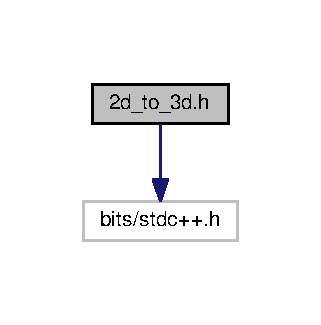
\includegraphics[width=154pt]{2d__to__3d_8h__incl}
\end{center}
\end{figure}
This graph shows which files directly or indirectly include this file\+:
\nopagebreak
\begin{figure}[H]
\begin{center}
\leavevmode
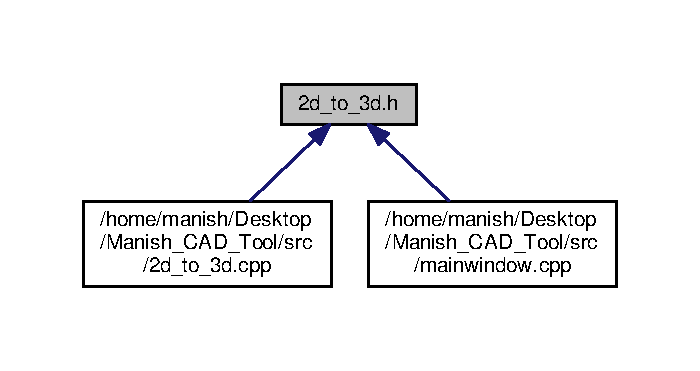
\includegraphics[width=336pt]{2d__to__3d_8h__dep__incl}
\end{center}
\end{figure}
\subsection*{Functions}
\begin{DoxyCompactItemize}
\item 
int \hyperlink{2d__to__3d_8h_a9782960d80f307ea5c1f83f61869f010}{two\+\_\+d\+\_\+to\+\_\+three\+\_\+d} (std\+::string file, std\+::string out\+File)
\end{DoxyCompactItemize}


\subsection{Function Documentation}
\index{2d\+\_\+to\+\_\+3d.\+h@{2d\+\_\+to\+\_\+3d.\+h}!two\+\_\+d\+\_\+to\+\_\+three\+\_\+d@{two\+\_\+d\+\_\+to\+\_\+three\+\_\+d}}
\index{two\+\_\+d\+\_\+to\+\_\+three\+\_\+d@{two\+\_\+d\+\_\+to\+\_\+three\+\_\+d}!2d\+\_\+to\+\_\+3d.\+h@{2d\+\_\+to\+\_\+3d.\+h}}
\subsubsection[{\texorpdfstring{two\+\_\+d\+\_\+to\+\_\+three\+\_\+d(std\+::string file, std\+::string out\+File)}{two_d_to_three_d(std::string file, std::string outFile)}}]{\setlength{\rightskip}{0pt plus 5cm}int two\+\_\+d\+\_\+to\+\_\+three\+\_\+d (
\begin{DoxyParamCaption}
\item[{std\+::string}]{file, }
\item[{std\+::string}]{out\+File}
\end{DoxyParamCaption}
)}\hypertarget{2d__to__3d_8h_a9782960d80f307ea5c1f83f61869f010}{}\label{2d__to__3d_8h_a9782960d80f307ea5c1f83f61869f010}

\hypertarget{3d__to__2d_8h}{}\section{3d\+\_\+to\+\_\+2d.h File Reference}
\label{3d__to__2d_8h}\index{3d\+\_\+to\+\_\+2d.\+h@{3d\+\_\+to\+\_\+2d.\+h}}
{\ttfamily \#include $<$string$>$}\\*
{\ttfamily \#include $<$form.\+h$>$}\\*
Include dependency graph for 3d\+\_\+to\+\_\+2d.h\+:
\nopagebreak
\begin{figure}[H]
\begin{center}
\leavevmode
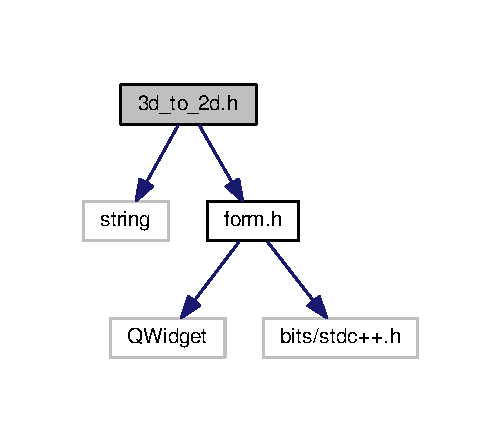
\includegraphics[width=241pt]{3d__to__2d_8h__incl}
\end{center}
\end{figure}
This graph shows which files directly or indirectly include this file\+:
\nopagebreak
\begin{figure}[H]
\begin{center}
\leavevmode
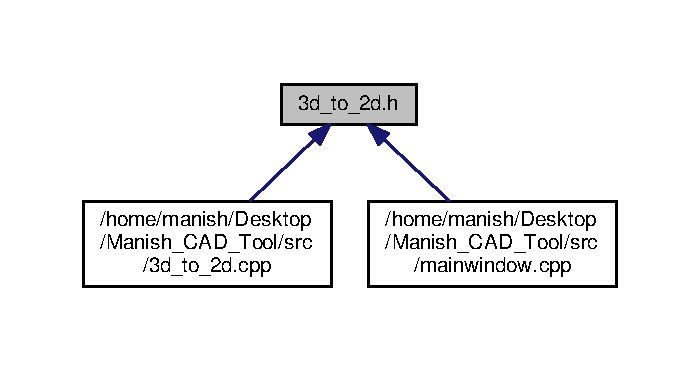
\includegraphics[width=336pt]{3d__to__2d_8h__dep__incl}
\end{center}
\end{figure}
\subsection*{Functions}
\begin{DoxyCompactItemize}
\item 
int \hyperlink{3d__to__2d_8h_a91c062617e686269181e084b4a340cd3}{three\+\_\+d\+\_\+to\+\_\+two\+\_\+d} (std\+::string a)
\end{DoxyCompactItemize}


\subsection{Function Documentation}
\index{3d\+\_\+to\+\_\+2d.\+h@{3d\+\_\+to\+\_\+2d.\+h}!three\+\_\+d\+\_\+to\+\_\+two\+\_\+d@{three\+\_\+d\+\_\+to\+\_\+two\+\_\+d}}
\index{three\+\_\+d\+\_\+to\+\_\+two\+\_\+d@{three\+\_\+d\+\_\+to\+\_\+two\+\_\+d}!3d\+\_\+to\+\_\+2d.\+h@{3d\+\_\+to\+\_\+2d.\+h}}
\subsubsection[{\texorpdfstring{three\+\_\+d\+\_\+to\+\_\+two\+\_\+d(std\+::string a)}{three_d_to_two_d(std::string a)}}]{\setlength{\rightskip}{0pt plus 5cm}int three\+\_\+d\+\_\+to\+\_\+two\+\_\+d (
\begin{DoxyParamCaption}
\item[{std\+::string}]{a}
\end{DoxyParamCaption}
)}\hypertarget{3d__to__2d_8h_a91c062617e686269181e084b4a340cd3}{}\label{3d__to__2d_8h_a91c062617e686269181e084b4a340cd3}

\hypertarget{body__loop_8h}{}\section{body\+\_\+loop.\+h File Reference}
\label{body__loop_8h}\index{body\+\_\+loop.\+h@{body\+\_\+loop.\+h}}
{\ttfamily \#include \char`\"{}structs.\+h\char`\"{}}\\*
{\ttfamily \#include \char`\"{}faceloop\+\_\+generator.\+h\char`\"{}}\\*
{\ttfamily \#include $<$vector$>$}\\*
{\ttfamily \#include $<$utility$>$}\\*
Include dependency graph for body\+\_\+loop.\+h\+:
\nopagebreak
\begin{figure}[H]
\begin{center}
\leavevmode
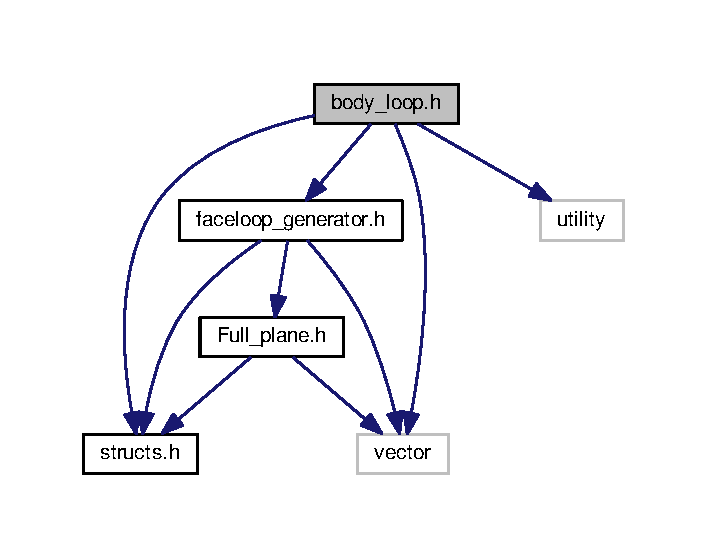
\includegraphics[width=340pt]{body__loop_8h__incl}
\end{center}
\end{figure}
This graph shows which files directly or indirectly include this file\+:
\nopagebreak
\begin{figure}[H]
\begin{center}
\leavevmode
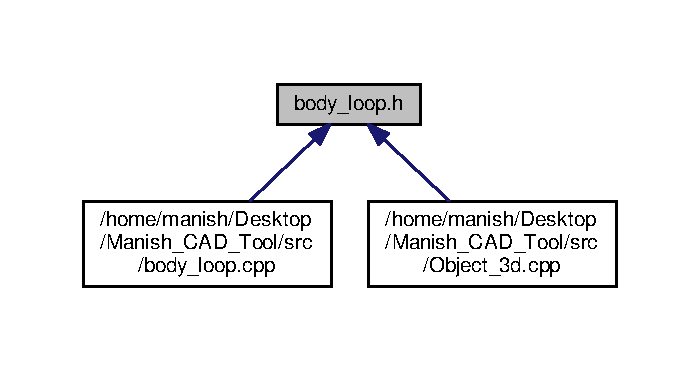
\includegraphics[width=336pt]{body__loop_8h__dep__incl}
\end{center}
\end{figure}
\subsection*{Classes}
\begin{DoxyCompactItemize}
\item 
class \hyperlink{classbody__loop}{body\+\_\+loop}
\end{DoxyCompactItemize}
\subsection*{Functions}
\begin{DoxyCompactItemize}
\item 
std\+::vector$<$ \hyperlink{classbody__loop}{body\+\_\+loop} $>$ \hyperlink{body__loop_8h_a230720d5c9d1a2805c6c743287d28d5b}{generate\+\_\+body\+\_\+loop} (std\+::vector$<$ \hyperlink{classface__loop}{face\+\_\+loop} $>$ face\+\_\+loop\+\_\+list, std\+::vector$<$ \hyperlink{classvertex__3d}{vertex\+\_\+3d} $>$ v3d\+\_\+list)
\item 
pair$<$ int, bool $>$ \hyperlink{body__loop_8h_a85f5918713a8c62784797c5766195628}{successive\+\_\+face\+\_\+loop} (std\+::vector$<$ \hyperlink{classface__loop}{face\+\_\+loop} $>$ face\+\_\+loop\+\_\+list, \hyperlink{classface__loop}{face\+\_\+loop} fl, int fl\+\_\+int, bool side, \hyperlink{classedge__3d}{edge\+\_\+3d} e, std\+::vector$<$ \hyperlink{classvertex__3d}{vertex\+\_\+3d} $>$ v3d\+\_\+list, bool inner\+\_\+basic)
\item 
void \hyperlink{body__loop_8h_af9a0c6603771f19b48cb31a570811386}{initialize\+\_\+side\+\_\+used} (std\+::vector$<$ pair$<$ bool, bool $>$ $>$ \&side\+\_\+used)
\begin{DoxyCompactList}\small\item\em function that initializes side\+\_\+used for both sides + and -\/ for every body loop \end{DoxyCompactList}\item 
bool \hyperlink{body__loop_8h_a0378c493f0dba980e5de09d11f03f447}{check\+\_\+legality} (\hyperlink{classbody__loop}{body\+\_\+loop} bp)
\begin{DoxyCompactList}\small\item\em function that checks that if a body part generated is legal or not \end{DoxyCompactList}\item 
bool \hyperlink{body__loop_8h_a68ebe3fd8487bbca7800bd67b4386970}{inner\+\_\+outer} (\hyperlink{classbody__loop}{body\+\_\+loop} bp, std\+::vector$<$ \hyperlink{classvertex__3d}{vertex\+\_\+3d} $>$ v3d\+\_\+list)
\begin{DoxyCompactList}\small\item\em function that determines if give body loop is inner or outer \end{DoxyCompactList}\item 
std\+::vector$<$ float $>$ \hyperlink{body__loop_8h_ad8e1589cd5ef438b41ebcce9fc970049}{get\+\_\+ray\+\_\+l} (\hyperlink{classplane}{plane} p1, \hyperlink{classplane}{plane} p2, bool s1, bool s2)
\begin{DoxyCompactList}\small\item\em function that determines vector along ray l = /$\vert$n1$\vert$ + /$\vert$n2$\vert$, where @ is the corresponding side \end{DoxyCompactList}\end{DoxyCompactItemize}


\subsection{Function Documentation}
\index{body\+\_\+loop.\+h@{body\+\_\+loop.\+h}!check\+\_\+legality@{check\+\_\+legality}}
\index{check\+\_\+legality@{check\+\_\+legality}!body\+\_\+loop.\+h@{body\+\_\+loop.\+h}}
\subsubsection[{\texorpdfstring{check\+\_\+legality(body\+\_\+loop bp)}{check_legality(body_loop bp)}}]{\setlength{\rightskip}{0pt plus 5cm}bool check\+\_\+legality (
\begin{DoxyParamCaption}
\item[{{\bf body\+\_\+loop}}]{bp}
\end{DoxyParamCaption}
)}\hypertarget{body__loop_8h_a0378c493f0dba980e5de09d11f03f447}{}\label{body__loop_8h_a0378c493f0dba980e5de09d11f03f447}


function that checks that if a body part generated is legal or not 



Definition at line 160 of file body\+\_\+loop.\+cpp.

\index{body\+\_\+loop.\+h@{body\+\_\+loop.\+h}!generate\+\_\+body\+\_\+loop@{generate\+\_\+body\+\_\+loop}}
\index{generate\+\_\+body\+\_\+loop@{generate\+\_\+body\+\_\+loop}!body\+\_\+loop.\+h@{body\+\_\+loop.\+h}}
\subsubsection[{\texorpdfstring{generate\+\_\+body\+\_\+loop(std\+::vector$<$ face\+\_\+loop $>$ face\+\_\+loop\+\_\+list, std\+::vector$<$ vertex\+\_\+3d $>$ v3d\+\_\+list)}{generate_body_loop(std::vector< face_loop > face_loop_list, std::vector< vertex_3d > v3d_list)}}]{\setlength{\rightskip}{0pt plus 5cm}std\+::vector$<$ {\bf body\+\_\+loop} $>$ generate\+\_\+body\+\_\+loop (
\begin{DoxyParamCaption}
\item[{std\+::vector$<$ {\bf face\+\_\+loop} $>$}]{face\+\_\+loop\+\_\+list, }
\item[{std\+::vector$<$ {\bf vertex\+\_\+3d} $>$}]{v3d\+\_\+list}
\end{DoxyParamCaption}
)}\hypertarget{body__loop_8h_a230720d5c9d1a2805c6c743287d28d5b}{}\label{body__loop_8h_a230720d5c9d1a2805c6c743287d28d5b}

\begin{DoxyParams}{Parameters}
{\em face\+\_\+loop\+\_\+list} & list of all face loops generated for the reconstruction \\
\hline
{\em v3d\+\_\+list} & vector of the 3d-\/vertices of the 3D object \\
\hline
\end{DoxyParams}


Definition at line 33 of file body\+\_\+loop.\+cpp.

\index{body\+\_\+loop.\+h@{body\+\_\+loop.\+h}!get\+\_\+ray\+\_\+l@{get\+\_\+ray\+\_\+l}}
\index{get\+\_\+ray\+\_\+l@{get\+\_\+ray\+\_\+l}!body\+\_\+loop.\+h@{body\+\_\+loop.\+h}}
\subsubsection[{\texorpdfstring{get\+\_\+ray\+\_\+l(plane p1, plane p2, bool s1, bool s2)}{get_ray_l(plane p1, plane p2, bool s1, bool s2)}}]{\setlength{\rightskip}{0pt plus 5cm}std\+::vector$<$float$>$ get\+\_\+ray\+\_\+l (
\begin{DoxyParamCaption}
\item[{{\bf plane}}]{p1, }
\item[{{\bf plane}}]{p2, }
\item[{bool}]{s1, }
\item[{bool}]{s2}
\end{DoxyParamCaption}
)}\hypertarget{body__loop_8h_ad8e1589cd5ef438b41ebcce9fc970049}{}\label{body__loop_8h_ad8e1589cd5ef438b41ebcce9fc970049}


function that determines vector along ray l = /$\vert$n1$\vert$ + /$\vert$n2$\vert$, where @ is the corresponding side 



Definition at line 187 of file body\+\_\+loop.\+cpp.

\index{body\+\_\+loop.\+h@{body\+\_\+loop.\+h}!initialize\+\_\+side\+\_\+used@{initialize\+\_\+side\+\_\+used}}
\index{initialize\+\_\+side\+\_\+used@{initialize\+\_\+side\+\_\+used}!body\+\_\+loop.\+h@{body\+\_\+loop.\+h}}
\subsubsection[{\texorpdfstring{initialize\+\_\+side\+\_\+used(std\+::vector$<$ pair$<$ bool, bool $>$ $>$ \&side\+\_\+used)}{initialize_side_used(std::vector< pair< bool, bool > > &side_used)}}]{\setlength{\rightskip}{0pt plus 5cm}void initialize\+\_\+side\+\_\+used (
\begin{DoxyParamCaption}
\item[{std\+::vector$<$ pair$<$ bool, bool $>$ $>$ \&}]{side\+\_\+used}
\end{DoxyParamCaption}
)}\hypertarget{body__loop_8h_af9a0c6603771f19b48cb31a570811386}{}\label{body__loop_8h_af9a0c6603771f19b48cb31a570811386}


function that initializes side\+\_\+used for both sides + and -\/ for every body loop 



Definition at line 152 of file body\+\_\+loop.\+cpp.

\index{body\+\_\+loop.\+h@{body\+\_\+loop.\+h}!inner\+\_\+outer@{inner\+\_\+outer}}
\index{inner\+\_\+outer@{inner\+\_\+outer}!body\+\_\+loop.\+h@{body\+\_\+loop.\+h}}
\subsubsection[{\texorpdfstring{inner\+\_\+outer(body\+\_\+loop bp, std\+::vector$<$ vertex\+\_\+3d $>$ v3d\+\_\+list)}{inner_outer(body_loop bp, std::vector< vertex_3d > v3d_list)}}]{\setlength{\rightskip}{0pt plus 5cm}bool inner\+\_\+outer (
\begin{DoxyParamCaption}
\item[{{\bf body\+\_\+loop}}]{bp, }
\item[{std\+::vector$<$ {\bf vertex\+\_\+3d} $>$}]{v3d\+\_\+list}
\end{DoxyParamCaption}
)}\hypertarget{body__loop_8h_a68ebe3fd8487bbca7800bd67b4386970}{}\label{body__loop_8h_a68ebe3fd8487bbca7800bd67b4386970}


function that determines if give body loop is inner or outer 



Definition at line 180 of file body\+\_\+loop.\+cpp.

\index{body\+\_\+loop.\+h@{body\+\_\+loop.\+h}!successive\+\_\+face\+\_\+loop@{successive\+\_\+face\+\_\+loop}}
\index{successive\+\_\+face\+\_\+loop@{successive\+\_\+face\+\_\+loop}!body\+\_\+loop.\+h@{body\+\_\+loop.\+h}}
\subsubsection[{\texorpdfstring{successive\+\_\+face\+\_\+loop(std\+::vector$<$ face\+\_\+loop $>$ face\+\_\+loop\+\_\+list, face\+\_\+loop fl, int fl\+\_\+int, bool side, edge\+\_\+3d e, std\+::vector$<$ vertex\+\_\+3d $>$ v3d\+\_\+list, bool inner\+\_\+basic)}{successive_face_loop(std::vector< face_loop > face_loop_list, face_loop fl, int fl_int, bool side, edge_3d e, std::vector< vertex_3d > v3d_list, bool inner_basic)}}]{\setlength{\rightskip}{0pt plus 5cm}pair$<$int,bool$>$ successive\+\_\+face\+\_\+loop (
\begin{DoxyParamCaption}
\item[{std\+::vector$<$ {\bf face\+\_\+loop} $>$}]{face\+\_\+loop\+\_\+list, }
\item[{{\bf face\+\_\+loop}}]{fl, }
\item[{int}]{fl\+\_\+int, }
\item[{bool}]{side, }
\item[{{\bf edge\+\_\+3d}}]{e, }
\item[{std\+::vector$<$ {\bf vertex\+\_\+3d} $>$}]{v3d\+\_\+list, }
\item[{bool}]{inner\+\_\+basic}
\end{DoxyParamCaption}
)}\hypertarget{body__loop_8h_a85f5918713a8c62784797c5766195628}{}\label{body__loop_8h_a85f5918713a8c62784797c5766195628}

\begin{DoxyParams}{Parameters}
{\em face\+\_\+loop\+\_\+list} & list of all face loops of the object \\
\hline
{\em fl} & face loop for which successive face loop is being found \\
\hline
{\em side} & side of the face loop (i.\+e + or -\/) \\
\hline
{\em e} & edge of the face loop fl at which successive face loop has to be found \\
\hline
{\em e\+\_\+vector} & 3$\ast$1 vector for direction of the edge e \\
\hline
\end{DoxyParams}
\begin{DoxyReturn}{Returns}
the index of successive face loop and its side 
\end{DoxyReturn}


Definition at line 111 of file body\+\_\+loop.\+cpp.


\hypertarget{faceloop__generator_8h}{}\section{faceloop\+\_\+generator.\+h File Reference}
\label{faceloop__generator_8h}\index{faceloop\+\_\+generator.\+h@{faceloop\+\_\+generator.\+h}}
{\ttfamily \#include \char`\"{}structs.\+h\char`\"{}}\\*
{\ttfamily \#include \char`\"{}Full\+\_\+plane.\+h\char`\"{}}\\*
{\ttfamily \#include $<$vector$>$}\\*
Include dependency graph for faceloop\+\_\+generator.\+h\+:
\nopagebreak
\begin{figure}[H]
\begin{center}
\leavevmode
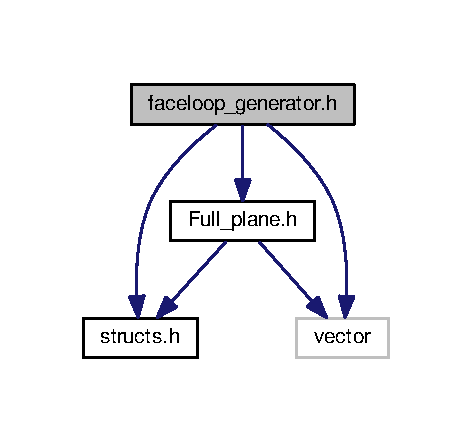
\includegraphics[width=227pt]{faceloop__generator_8h__incl}
\end{center}
\end{figure}
This graph shows which files directly or indirectly include this file\+:
\nopagebreak
\begin{figure}[H]
\begin{center}
\leavevmode
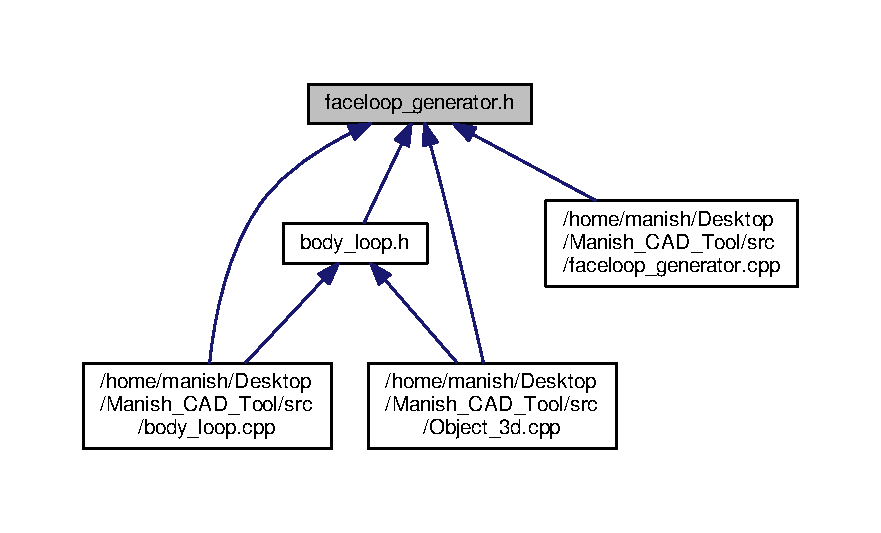
\includegraphics[width=350pt]{faceloop__generator_8h__dep__incl}
\end{center}
\end{figure}
\subsection*{Classes}
\begin{DoxyCompactItemize}
\item 
class \hyperlink{classbasic__loop}{basic\+\_\+loop}
\item 
class \hyperlink{classface__loop}{face\+\_\+loop}
\end{DoxyCompactItemize}
\subsection*{Functions}
\begin{DoxyCompactItemize}
\item 
std\+::vector$<$ \hyperlink{classface__loop}{face\+\_\+loop} $>$ \hyperlink{faceloop__generator_8h_ae6b709b480a42b239420e2f968bf4a6c}{generate\+\_\+face\+\_\+loops} (\hyperlink{classplane}{plane} p, std\+::vector$<$ int $>$ vertices\+\_\+on\+\_\+the\+\_\+plane, std\+::vector$<$ \hyperlink{classedge__3d}{edge\+\_\+3d} $>$ \&edges\+\_\+on\+\_\+the\+\_\+plane, std\+::vector$<$ \hyperlink{classvertex__3d}{vertex\+\_\+3d} $>$ v3d\+\_\+list)
\item 
std\+::vector$<$ std\+::vector$<$ int $>$ $>$ \hyperlink{faceloop__generator_8h_aadb442650ebd831d3c7fda4a627d1ace}{generate\+\_\+ordered\+\_\+adj\+\_\+list} (std\+::vector$<$ \hyperlink{classedge__3d}{edge\+\_\+3d} $>$ edges\+\_\+on\+\_\+the\+\_\+plane, std\+::vector$<$ int $>$ vertices\+\_\+on\+\_\+the\+\_\+plane, std\+::vector$<$ \hyperlink{classvertex__3d}{vertex\+\_\+3d} $>$ v3d\+\_\+list)
\begin{DoxyCompactList}\small\item\em function to generate ordered adj\+\_\+list in clockwise direction \end{DoxyCompactList}\item 
std\+::vector$<$ \hyperlink{classbasic__loop}{basic\+\_\+loop} $>$ \hyperlink{faceloop__generator_8h_a7a4a04f233606e5f06164dc9a97b47a5}{basic\+\_\+loop\+\_\+generator} (std\+::vector$<$ \hyperlink{classedge__3d}{edge\+\_\+3d} $>$ \&edges\+\_\+on\+\_\+the\+\_\+plane, std\+::vector$<$ vector$<$ int $>$ $>$ ordered\+\_\+adj\+\_\+list)
\begin{DoxyCompactList}\small\item\em function that generates basic loops \end{DoxyCompactList}\item 
std\+::vector$<$ std\+::vector$<$ bool $>$ $>$ \hyperlink{faceloop__generator_8h_a9a32da1f4ab031ab685165a2ac99dab8}{generate\+\_\+inclusion\+\_\+matrix} (std\+::vector$<$ \hyperlink{classbasic__loop}{basic\+\_\+loop} $>$ basic\+\_\+loop\+\_\+list, std\+::vector$<$ \hyperlink{classvertex__3d}{vertex\+\_\+3d} $>$ v3d\+\_\+list)
\begin{DoxyCompactList}\small\item\em function to generate inclusion matrix \end{DoxyCompactList}\end{DoxyCompactItemize}


\subsection{Function Documentation}
\index{faceloop\+\_\+generator.\+h@{faceloop\+\_\+generator.\+h}!basic\+\_\+loop\+\_\+generator@{basic\+\_\+loop\+\_\+generator}}
\index{basic\+\_\+loop\+\_\+generator@{basic\+\_\+loop\+\_\+generator}!faceloop\+\_\+generator.\+h@{faceloop\+\_\+generator.\+h}}
\subsubsection[{\texorpdfstring{basic\+\_\+loop\+\_\+generator(std\+::vector$<$ edge\+\_\+3d $>$ \&edges\+\_\+on\+\_\+the\+\_\+plane, std\+::vector$<$ vector$<$ int $>$ $>$ ordered\+\_\+adj\+\_\+list)}{basic_loop_generator(std::vector< edge_3d > &edges_on_the_plane, std::vector< vector< int > > ordered_adj_list)}}]{\setlength{\rightskip}{0pt plus 5cm}std\+::vector$<$ {\bf basic\+\_\+loop} $>$ basic\+\_\+loop\+\_\+generator (
\begin{DoxyParamCaption}
\item[{std\+::vector$<$ {\bf edge\+\_\+3d} $>$ \&}]{edges\+\_\+on\+\_\+the\+\_\+plane, }
\item[{std\+::vector$<$ vector$<$ int $>$ $>$}]{ordered\+\_\+adj\+\_\+list}
\end{DoxyParamCaption}
)}\hypertarget{faceloop__generator_8h_a7a4a04f233606e5f06164dc9a97b47a5}{}\label{faceloop__generator_8h_a7a4a04f233606e5f06164dc9a97b47a5}


function that generates basic loops 



Definition at line 168 of file faceloop\+\_\+generator.\+cpp.

\index{faceloop\+\_\+generator.\+h@{faceloop\+\_\+generator.\+h}!generate\+\_\+face\+\_\+loops@{generate\+\_\+face\+\_\+loops}}
\index{generate\+\_\+face\+\_\+loops@{generate\+\_\+face\+\_\+loops}!faceloop\+\_\+generator.\+h@{faceloop\+\_\+generator.\+h}}
\subsubsection[{\texorpdfstring{generate\+\_\+face\+\_\+loops(plane p, std\+::vector$<$ int $>$ vertices\+\_\+on\+\_\+the\+\_\+plane, std\+::vector$<$ edge\+\_\+3d $>$ \&edges\+\_\+on\+\_\+the\+\_\+plane, std\+::vector$<$ vertex\+\_\+3d $>$ v3d\+\_\+list)}{generate_face_loops(plane p, std::vector< int > vertices_on_the_plane, std::vector< edge_3d > &edges_on_the_plane, std::vector< vertex_3d > v3d_list)}}]{\setlength{\rightskip}{0pt plus 5cm}std\+::vector$<$ {\bf face\+\_\+loop} $>$ generate\+\_\+face\+\_\+loops (
\begin{DoxyParamCaption}
\item[{{\bf plane}}]{p, }
\item[{std\+::vector$<$ int $>$}]{vertices\+\_\+on\+\_\+the\+\_\+plane, }
\item[{std\+::vector$<$ {\bf edge\+\_\+3d} $>$ \&}]{edges\+\_\+on\+\_\+the\+\_\+plane, }
\item[{std\+::vector$<$ {\bf vertex\+\_\+3d} $>$}]{v3d\+\_\+list}
\end{DoxyParamCaption}
)}\hypertarget{faceloop__generator_8h_ae6b709b480a42b239420e2f968bf4a6c}{}\label{faceloop__generator_8h_ae6b709b480a42b239420e2f968bf4a6c}

\begin{DoxyParams}{Parameters}
{\em p} & plane for which face\+\_\+loops are being calculated \\
\hline
{\em edges\+\_\+on\+\_\+the\+\_\+plane} & vector of the edges which are on this plane \\
\hline
{\em v3d\+\_\+list} & vertex list of the 3d object \\
\hline
\end{DoxyParams}


Definition at line 36 of file faceloop\+\_\+generator.\+cpp.

\index{faceloop\+\_\+generator.\+h@{faceloop\+\_\+generator.\+h}!generate\+\_\+inclusion\+\_\+matrix@{generate\+\_\+inclusion\+\_\+matrix}}
\index{generate\+\_\+inclusion\+\_\+matrix@{generate\+\_\+inclusion\+\_\+matrix}!faceloop\+\_\+generator.\+h@{faceloop\+\_\+generator.\+h}}
\subsubsection[{\texorpdfstring{generate\+\_\+inclusion\+\_\+matrix(std\+::vector$<$ basic\+\_\+loop $>$ basic\+\_\+loop\+\_\+list, std\+::vector$<$ vertex\+\_\+3d $>$ v3d\+\_\+list)}{generate_inclusion_matrix(std::vector< basic_loop > basic_loop_list, std::vector< vertex_3d > v3d_list)}}]{\setlength{\rightskip}{0pt plus 5cm}std\+::vector$<$ std\+::vector$<$bool$>$ $>$ generate\+\_\+inclusion\+\_\+matrix (
\begin{DoxyParamCaption}
\item[{std\+::vector$<$ {\bf basic\+\_\+loop} $>$}]{basic\+\_\+loop\+\_\+list, }
\item[{std\+::vector$<$ {\bf vertex\+\_\+3d} $>$}]{v3d\+\_\+list}
\end{DoxyParamCaption}
)}\hypertarget{faceloop__generator_8h_a9a32da1f4ab031ab685165a2ac99dab8}{}\label{faceloop__generator_8h_a9a32da1f4ab031ab685165a2ac99dab8}


function to generate inclusion matrix 



Definition at line 392 of file faceloop\+\_\+generator.\+cpp.

\index{faceloop\+\_\+generator.\+h@{faceloop\+\_\+generator.\+h}!generate\+\_\+ordered\+\_\+adj\+\_\+list@{generate\+\_\+ordered\+\_\+adj\+\_\+list}}
\index{generate\+\_\+ordered\+\_\+adj\+\_\+list@{generate\+\_\+ordered\+\_\+adj\+\_\+list}!faceloop\+\_\+generator.\+h@{faceloop\+\_\+generator.\+h}}
\subsubsection[{\texorpdfstring{generate\+\_\+ordered\+\_\+adj\+\_\+list(std\+::vector$<$ edge\+\_\+3d $>$ edges\+\_\+on\+\_\+the\+\_\+plane, std\+::vector$<$ int $>$ vertices\+\_\+on\+\_\+the\+\_\+plane, std\+::vector$<$ vertex\+\_\+3d $>$ v3d\+\_\+list)}{generate_ordered_adj_list(std::vector< edge_3d > edges_on_the_plane, std::vector< int > vertices_on_the_plane, std::vector< vertex_3d > v3d_list)}}]{\setlength{\rightskip}{0pt plus 5cm}std\+::vector$<$ std\+::vector$<$int$>$ $>$ generate\+\_\+ordered\+\_\+adj\+\_\+list (
\begin{DoxyParamCaption}
\item[{std\+::vector$<$ {\bf edge\+\_\+3d} $>$}]{edges\+\_\+on\+\_\+the\+\_\+plane, }
\item[{std\+::vector$<$ int $>$}]{vertices\+\_\+on\+\_\+the\+\_\+plane, }
\item[{std\+::vector$<$ {\bf vertex\+\_\+3d} $>$}]{v3d\+\_\+list}
\end{DoxyParamCaption}
)}\hypertarget{faceloop__generator_8h_aadb442650ebd831d3c7fda4a627d1ace}{}\label{faceloop__generator_8h_aadb442650ebd831d3c7fda4a627d1ace}


function to generate ordered adj\+\_\+list in clockwise direction 



Definition at line 152 of file faceloop\+\_\+generator.\+cpp.


\hypertarget{form_8h}{}\section{form.\+h File Reference}
\label{form_8h}\index{form.\+h@{form.\+h}}
{\ttfamily \#include $<$Q\+Widget$>$}\\*
{\ttfamily \#include $<$bits/stdc++.\+h$>$}\\*
Include dependency graph for form.\+h\+:
\nopagebreak
\begin{figure}[H]
\begin{center}
\leavevmode
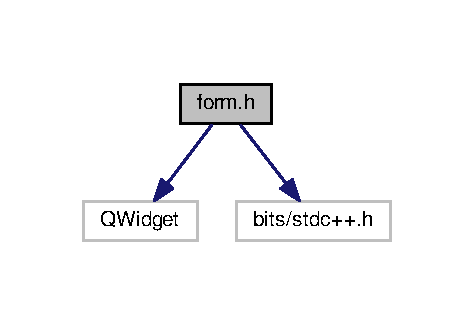
\includegraphics[width=228pt]{form_8h__incl}
\end{center}
\end{figure}
This graph shows which files directly or indirectly include this file\+:
\nopagebreak
\begin{figure}[H]
\begin{center}
\leavevmode
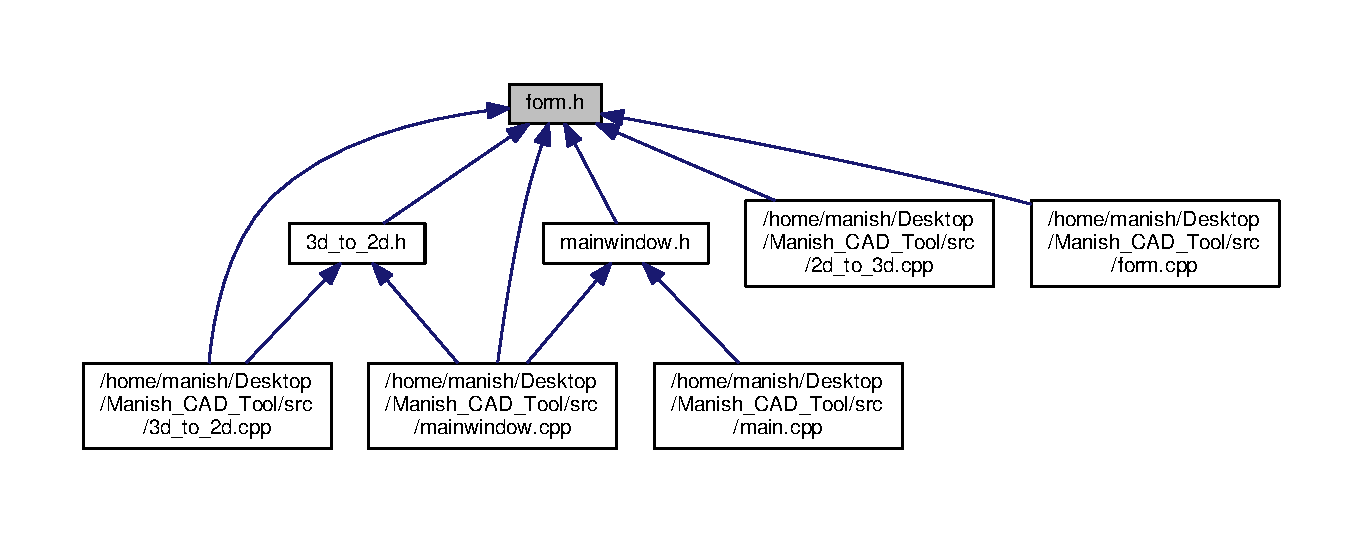
\includegraphics[width=350pt]{form_8h__dep__incl}
\end{center}
\end{figure}
\subsection*{Classes}
\begin{DoxyCompactItemize}
\item 
class \hyperlink{class_form}{Form}
\end{DoxyCompactItemize}
\subsection*{Namespaces}
\begin{DoxyCompactItemize}
\item 
 \hyperlink{namespace_ui}{Ui}
\end{DoxyCompactItemize}

\hypertarget{_full__plane_8h}{}\section{Full\+\_\+plane.\+h File Reference}
\label{_full__plane_8h}\index{Full\+\_\+plane.\+h@{Full\+\_\+plane.\+h}}
{\ttfamily \#include $<$vector$>$}\\*
{\ttfamily \#include \char`\"{}structs.\+h\char`\"{}}\\*
Include dependency graph for Full\+\_\+plane.\+h\+:
\nopagebreak
\begin{figure}[H]
\begin{center}
\leavevmode
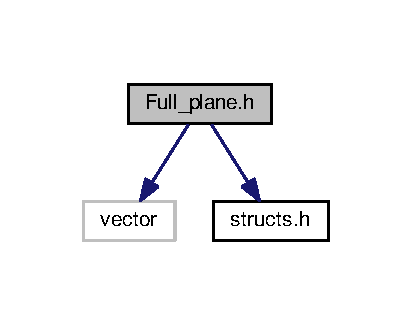
\includegraphics[width=198pt]{_full__plane_8h__incl}
\end{center}
\end{figure}
This graph shows which files directly or indirectly include this file\+:
\nopagebreak
\begin{figure}[H]
\begin{center}
\leavevmode
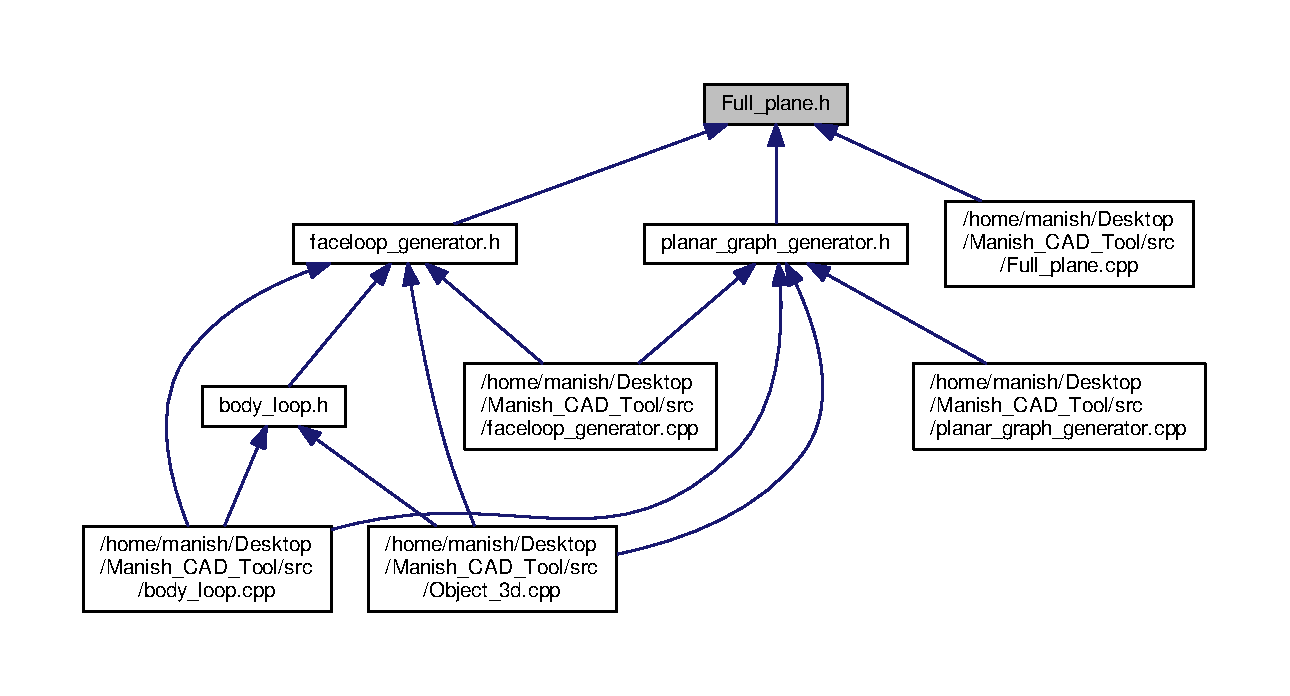
\includegraphics[width=350pt]{_full__plane_8h__dep__incl}
\end{center}
\end{figure}
\subsection*{Classes}
\begin{DoxyCompactItemize}
\item 
class \hyperlink{class_full__plane}{Full\+\_\+plane}
\end{DoxyCompactItemize}

\hypertarget{general__methods_8h}{}\section{general\+\_\+methods.\+h File Reference}
\label{general__methods_8h}\index{general\+\_\+methods.\+h@{general\+\_\+methods.\+h}}
{\ttfamily \#include \char`\"{}structs.\+h\char`\"{}}\\*
Include dependency graph for general\+\_\+methods.\+h\+:
\nopagebreak
\begin{figure}[H]
\begin{center}
\leavevmode
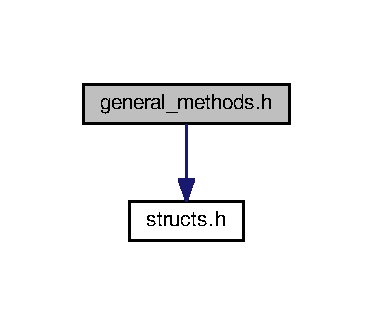
\includegraphics[width=179pt]{general__methods_8h__incl}
\end{center}
\end{figure}
This graph shows which files directly or indirectly include this file\+:
\nopagebreak
\begin{figure}[H]
\begin{center}
\leavevmode
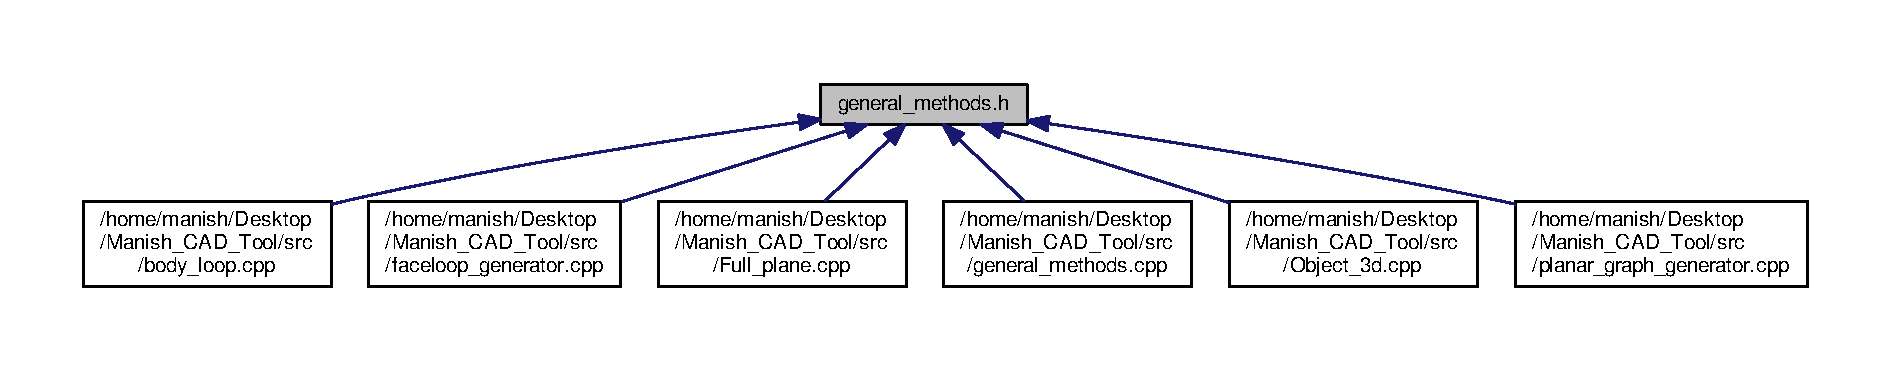
\includegraphics[width=350pt]{general__methods_8h__dep__incl}
\end{center}
\end{figure}
\subsection*{Functions}
\begin{DoxyCompactItemize}
\item 
\hyperlink{classvertex__3d}{vertex\+\_\+3d} \hyperlink{general__methods_8h_a2dc9a47107e3f17fb944f6077f942236}{cross\+\_\+product} (\hyperlink{classvertex__3d}{vertex\+\_\+3d} a, \hyperlink{classvertex__3d}{vertex\+\_\+3d} b)
\item 
float \hyperlink{general__methods_8h_adde63ba9542357791cc6a967f2ea582e}{dot\+\_\+product} (\hyperlink{classvertex__3d}{vertex\+\_\+3d} a, \hyperlink{classvertex__3d}{vertex\+\_\+3d} b)
\end{DoxyCompactItemize}


\subsection{Function Documentation}
\index{general\+\_\+methods.\+h@{general\+\_\+methods.\+h}!cross\+\_\+product@{cross\+\_\+product}}
\index{cross\+\_\+product@{cross\+\_\+product}!general\+\_\+methods.\+h@{general\+\_\+methods.\+h}}
\subsubsection[{\texorpdfstring{cross\+\_\+product(vertex\+\_\+3d a, vertex\+\_\+3d b)}{cross_product(vertex_3d a, vertex_3d b)}}]{\setlength{\rightskip}{0pt plus 5cm}{\bf vertex\+\_\+3d} cross\+\_\+product (
\begin{DoxyParamCaption}
\item[{{\bf vertex\+\_\+3d}}]{a, }
\item[{{\bf vertex\+\_\+3d}}]{b}
\end{DoxyParamCaption}
)}\hypertarget{general__methods_8h_a2dc9a47107e3f17fb944f6077f942236}{}\label{general__methods_8h_a2dc9a47107e3f17fb944f6077f942236}


Definition at line 5 of file general\+\_\+methods.\+cpp.

\index{general\+\_\+methods.\+h@{general\+\_\+methods.\+h}!dot\+\_\+product@{dot\+\_\+product}}
\index{dot\+\_\+product@{dot\+\_\+product}!general\+\_\+methods.\+h@{general\+\_\+methods.\+h}}
\subsubsection[{\texorpdfstring{dot\+\_\+product(vertex\+\_\+3d a, vertex\+\_\+3d b)}{dot_product(vertex_3d a, vertex_3d b)}}]{\setlength{\rightskip}{0pt plus 5cm}float dot\+\_\+product (
\begin{DoxyParamCaption}
\item[{{\bf vertex\+\_\+3d}}]{a, }
\item[{{\bf vertex\+\_\+3d}}]{b}
\end{DoxyParamCaption}
)}\hypertarget{general__methods_8h_adde63ba9542357791cc6a967f2ea582e}{}\label{general__methods_8h_adde63ba9542357791cc6a967f2ea582e}


Definition at line 17 of file general\+\_\+methods.\+cpp.


\hypertarget{mainwindow_8h}{}\section{mainwindow.\+h File Reference}
\label{mainwindow_8h}\index{mainwindow.\+h@{mainwindow.\+h}}
{\ttfamily \#include $<$Q\+Main\+Window$>$}\\*
{\ttfamily \#include \char`\"{}form.\+h\char`\"{}}\\*
Include dependency graph for mainwindow.\+h\+:
\nopagebreak
\begin{figure}[H]
\begin{center}
\leavevmode
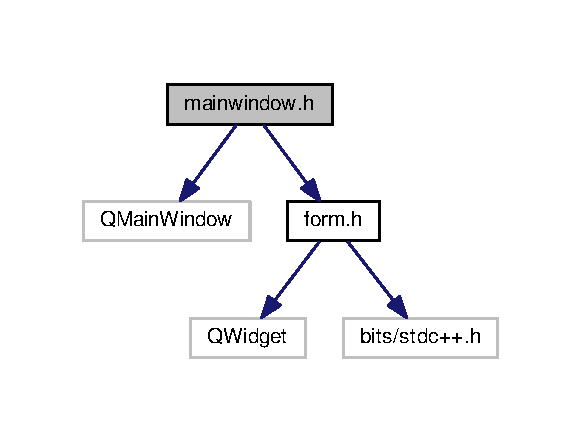
\includegraphics[width=279pt]{mainwindow_8h__incl}
\end{center}
\end{figure}
This graph shows which files directly or indirectly include this file\+:
\nopagebreak
\begin{figure}[H]
\begin{center}
\leavevmode
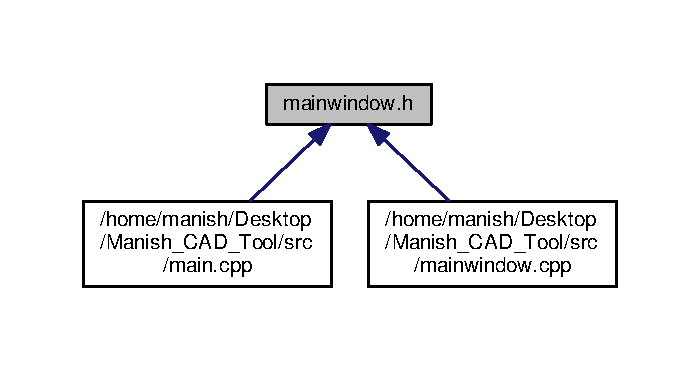
\includegraphics[width=336pt]{mainwindow_8h__dep__incl}
\end{center}
\end{figure}
\subsection*{Classes}
\begin{DoxyCompactItemize}
\item 
class \hyperlink{class_main_window}{Main\+Window}
\end{DoxyCompactItemize}
\subsection*{Namespaces}
\begin{DoxyCompactItemize}
\item 
 \hyperlink{namespace_ui}{Ui}
\end{DoxyCompactItemize}

\hypertarget{object__2d_8h}{}\section{object\+\_\+2d.\+h File Reference}
\label{object__2d_8h}\index{object\+\_\+2d.\+h@{object\+\_\+2d.\+h}}
{\ttfamily \#include \char`\"{}structs.\+h\char`\"{}}\\*
{\ttfamily \#include $<$vector$>$}\\*
Include dependency graph for object\+\_\+2d.\+h\+:
\nopagebreak
\begin{figure}[H]
\begin{center}
\leavevmode
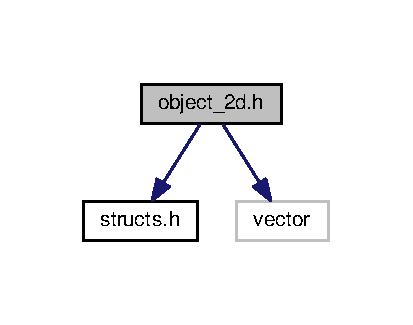
\includegraphics[width=198pt]{object__2d_8h__incl}
\end{center}
\end{figure}
This graph shows which files directly or indirectly include this file\+:
\nopagebreak
\begin{figure}[H]
\begin{center}
\leavevmode
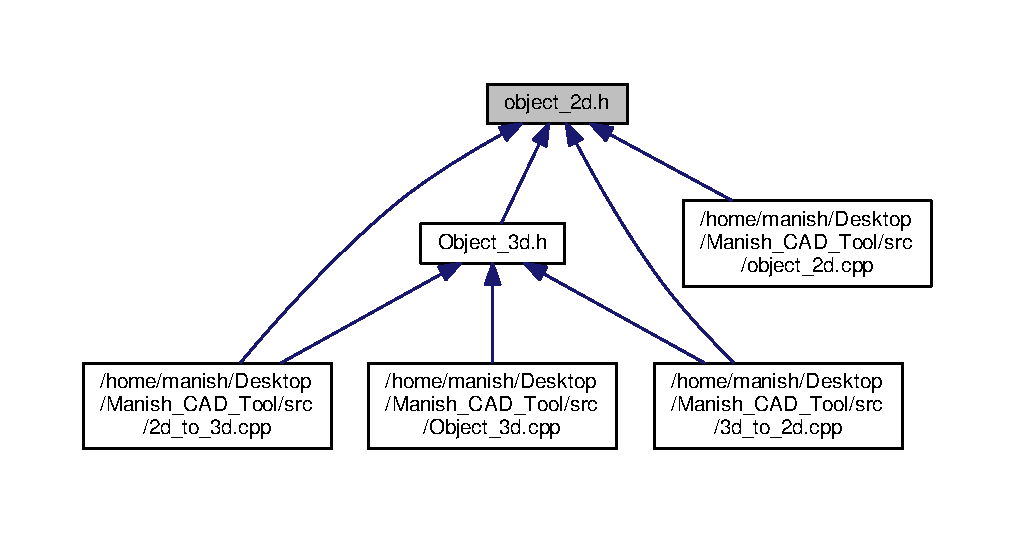
\includegraphics[width=350pt]{object__2d_8h__dep__incl}
\end{center}
\end{figure}
\subsection*{Classes}
\begin{DoxyCompactItemize}
\item 
class \hyperlink{classobject__2d}{object\+\_\+2d}
\begin{DoxyCompactList}\small\item\em representation of \hyperlink{classobject__2d}{object\+\_\+2d} \end{DoxyCompactList}\end{DoxyCompactItemize}

\hypertarget{_object__3d_8h}{}\section{Object\+\_\+3d.\+h File Reference}
\label{_object__3d_8h}\index{Object\+\_\+3d.\+h@{Object\+\_\+3d.\+h}}
{\ttfamily \#include \char`\"{}structs.\+h\char`\"{}}\\*
{\ttfamily \#include $<$vector$>$}\\*
{\ttfamily \#include \char`\"{}object\+\_\+2d.\+h\char`\"{}}\\*
Include dependency graph for Object\+\_\+3d.\+h\+:
\nopagebreak
\begin{figure}[H]
\begin{center}
\leavevmode
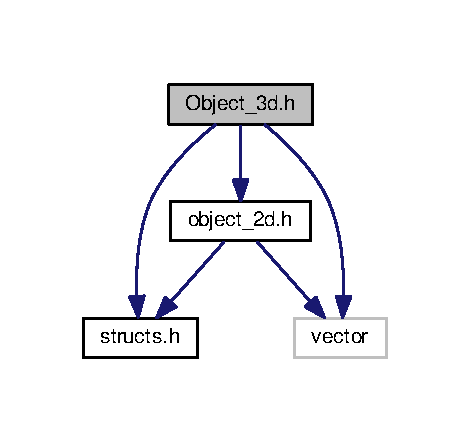
\includegraphics[width=226pt]{_object__3d_8h__incl}
\end{center}
\end{figure}
This graph shows which files directly or indirectly include this file\+:
\nopagebreak
\begin{figure}[H]
\begin{center}
\leavevmode
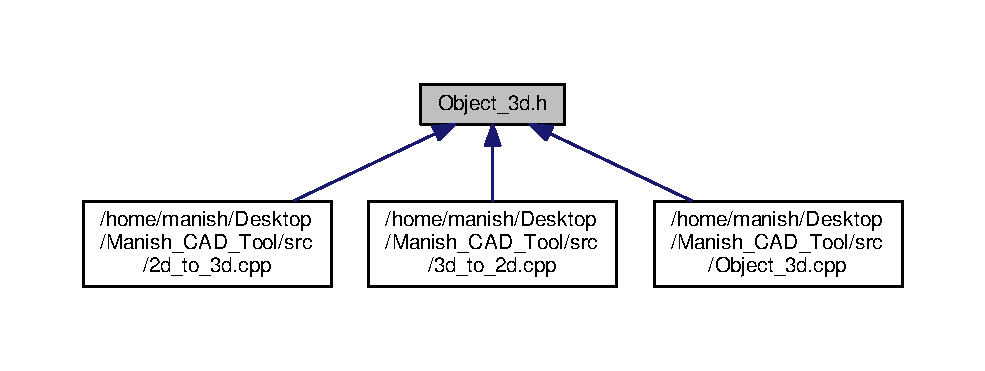
\includegraphics[width=350pt]{_object__3d_8h__dep__incl}
\end{center}
\end{figure}
\subsection*{Classes}
\begin{DoxyCompactItemize}
\item 
class \hyperlink{class_object__3d}{Object\+\_\+3d}
\end{DoxyCompactItemize}

\hypertarget{planar__graph__generator_8h}{}\section{planar\+\_\+graph\+\_\+generator.\+h File Reference}
\label{planar__graph__generator_8h}\index{planar\+\_\+graph\+\_\+generator.\+h@{planar\+\_\+graph\+\_\+generator.\+h}}
{\ttfamily \#include \char`\"{}structs.\+h\char`\"{}}\\*
{\ttfamily \#include \char`\"{}Full\+\_\+plane.\+h\char`\"{}}\\*
{\ttfamily \#include $<$vector$>$}\\*
Include dependency graph for planar\+\_\+graph\+\_\+generator.\+h\+:
\nopagebreak
\begin{figure}[H]
\begin{center}
\leavevmode
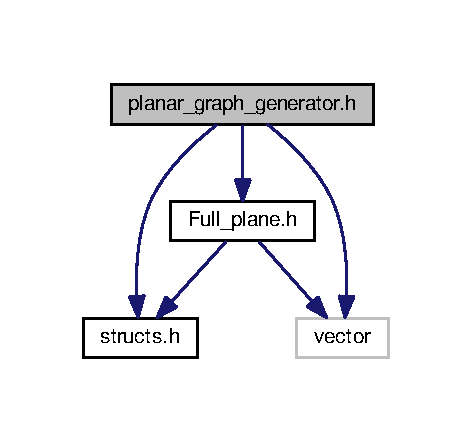
\includegraphics[width=227pt]{planar__graph__generator_8h__incl}
\end{center}
\end{figure}
This graph shows which files directly or indirectly include this file\+:
\nopagebreak
\begin{figure}[H]
\begin{center}
\leavevmode
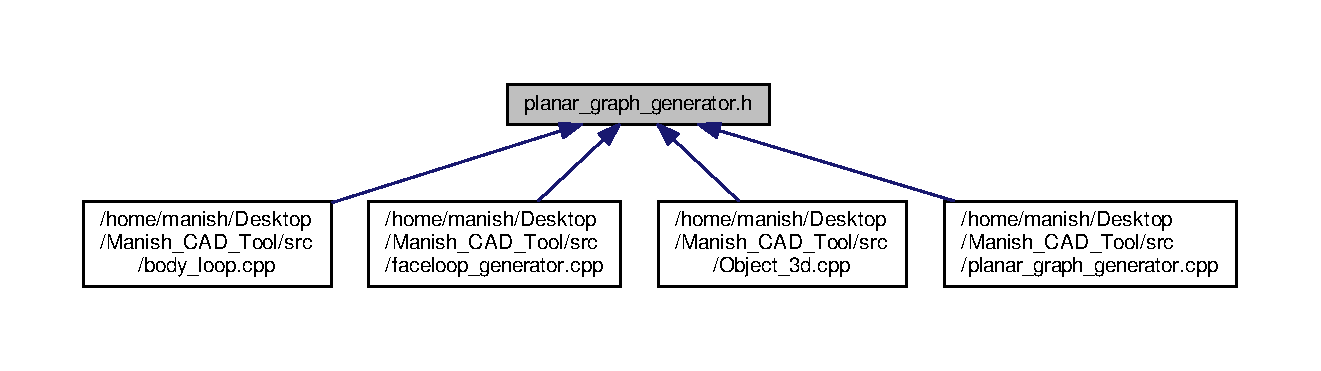
\includegraphics[width=350pt]{planar__graph__generator_8h__dep__incl}
\end{center}
\end{figure}
\subsection*{Functions}
\begin{DoxyCompactItemize}
\item 
std\+::vector$<$ \hyperlink{class_full__plane}{Full\+\_\+plane} $>$ \hyperlink{planar__graph__generator_8h_a2cdfdb8be2237b1c7359b630e9603cfd}{planar\+\_\+graph\+\_\+generator} (std\+::vector$<$ \hyperlink{classvertex__3d}{vertex\+\_\+3d} $>$ v3d\+\_\+list, std\+::vector$<$ \hyperlink{classedge__3d}{edge\+\_\+3d} $>$ \&e3d\+\_\+list)
\begin{DoxyCompactList}\small\item\em function that generates and retunrs planes \end{DoxyCompactList}\item 
std\+::vector$<$ \hyperlink{classplane}{plane} $>$ \hyperlink{planar__graph__generator_8h_a8d89f969b47445ac1b5b0cf170401cf1}{construct\+\_\+planes} (std\+::vector$<$ \hyperlink{classvertex__3d}{vertex\+\_\+3d} $>$ v3d\+\_\+list, std\+::vector$<$ \hyperlink{classedge__3d}{edge\+\_\+3d} $>$ e3d\+\_\+list, std\+::vector$<$ std\+::vector$<$ int $>$ $>$ adj\+\_\+list)
\begin{DoxyCompactList}\small\item\em function that constructs plane equations \end{DoxyCompactList}\item 
std\+::vector$<$ std\+::vector$<$ int $>$ $>$ \hyperlink{planar__graph__generator_8h_a077660a929dda9adf2f8a2daa6a563c1}{get\+\_\+adj\+\_\+list} (std\+::vector$<$ \hyperlink{classedge__3d}{edge\+\_\+3d} $>$ e3d\+\_\+list, int no\+\_\+of\+\_\+vertices)
\begin{DoxyCompactList}\small\item\em function that returns adjacency edges list of the \hyperlink{classvertex__3d}{vertex\+\_\+3d} list \end{DoxyCompactList}\item 
std\+::vector$<$ \hyperlink{classplane}{plane} $>$ \hyperlink{planar__graph__generator_8h_a488a27459d11af0b73b76ebe78a8a1c4}{eliminate\+\_\+duplicate\+\_\+planes} (std\+::vector$<$ \hyperlink{classplane}{plane} $>$ planes)
\begin{DoxyCompactList}\small\item\em function that eliminates duplicate formed planes \end{DoxyCompactList}\item 
bool \hyperlink{planar__graph__generator_8h_acd37db477f3dd31a46790f5a7ded851c}{check\+\_\+legality} (\hyperlink{class_full__plane}{Full\+\_\+plane} \&f, std\+::vector$<$ std\+::vector$<$ int $>$ $>$ adj\+\_\+list)
\begin{DoxyCompactList}\small\item\em function returns true if planar graph is legal \end{DoxyCompactList}\item 
void \hyperlink{planar__graph__generator_8h_a47eedebb44f45567710e54702a5f28b6}{remove\+\_\+dangling} (\hyperlink{class_full__plane}{Full\+\_\+plane} \&f, std\+::vector$<$ std\+::vector$<$ int $>$ $>$ adj\+\_\+list)
\begin{DoxyCompactList}\small\item\em function that removes dangling and isolated edges on the planar graph using dfs \end{DoxyCompactList}\item 
void \hyperlink{planar__graph__generator_8h_ad4d8aa255999d941dcc6b5b61ca9d0fd}{remove\+\_\+single\+\_\+plane\+\_\+edges} (std\+::vector$<$ \hyperlink{class_full__plane}{Full\+\_\+plane} $>$ \&f\+\_\+list, std\+::vector$<$ \hyperlink{classedge__3d}{edge\+\_\+3d} $>$ \&e3d\+\_\+list)
\begin{DoxyCompactList}\small\item\em function that removes those edges which belongs only to one planner graph \end{DoxyCompactList}\end{DoxyCompactItemize}


\subsection{Function Documentation}
\index{planar\+\_\+graph\+\_\+generator.\+h@{planar\+\_\+graph\+\_\+generator.\+h}!check\+\_\+legality@{check\+\_\+legality}}
\index{check\+\_\+legality@{check\+\_\+legality}!planar\+\_\+graph\+\_\+generator.\+h@{planar\+\_\+graph\+\_\+generator.\+h}}
\subsubsection[{\texorpdfstring{check\+\_\+legality(\+Full\+\_\+plane \&f, std\+::vector$<$ std\+::vector$<$ int $>$ $>$ adj\+\_\+list)}{check_legality(Full_plane &f, std::vector< std::vector< int > > adj_list)}}]{\setlength{\rightskip}{0pt plus 5cm}bool check\+\_\+legality (
\begin{DoxyParamCaption}
\item[{{\bf Full\+\_\+plane} \&}]{f, }
\item[{std\+::vector$<$ std\+::vector$<$ int $>$ $>$}]{adj\+\_\+list}
\end{DoxyParamCaption}
)}\hypertarget{planar__graph__generator_8h_acd37db477f3dd31a46790f5a7ded851c}{}\label{planar__graph__generator_8h_acd37db477f3dd31a46790f5a7ded851c}


function returns true if planar graph is legal 



Definition at line 80 of file planar\+\_\+graph\+\_\+generator.\+cpp.

\index{planar\+\_\+graph\+\_\+generator.\+h@{planar\+\_\+graph\+\_\+generator.\+h}!construct\+\_\+planes@{construct\+\_\+planes}}
\index{construct\+\_\+planes@{construct\+\_\+planes}!planar\+\_\+graph\+\_\+generator.\+h@{planar\+\_\+graph\+\_\+generator.\+h}}
\subsubsection[{\texorpdfstring{construct\+\_\+planes(std\+::vector$<$ vertex\+\_\+3d $>$ v3d\+\_\+list, std\+::vector$<$ edge\+\_\+3d $>$ e3d\+\_\+list, std\+::vector$<$ std\+::vector$<$ int $>$ $>$ adj\+\_\+list)}{construct_planes(std::vector< vertex_3d > v3d_list, std::vector< edge_3d > e3d_list, std::vector< std::vector< int > > adj_list)}}]{\setlength{\rightskip}{0pt plus 5cm}std\+::vector$<$ {\bf plane} $>$ construct\+\_\+planes (
\begin{DoxyParamCaption}
\item[{std\+::vector$<$ {\bf vertex\+\_\+3d} $>$}]{v3d\+\_\+list, }
\item[{std\+::vector$<$ {\bf edge\+\_\+3d} $>$}]{e3d\+\_\+list, }
\item[{std\+::vector$<$ std\+::vector$<$ int $>$ $>$}]{adj\+\_\+list}
\end{DoxyParamCaption}
)}\hypertarget{planar__graph__generator_8h_a8d89f969b47445ac1b5b0cf170401cf1}{}\label{planar__graph__generator_8h_a8d89f969b47445ac1b5b0cf170401cf1}


function that constructs plane equations 



Definition at line 27 of file planar\+\_\+graph\+\_\+generator.\+cpp.

\index{planar\+\_\+graph\+\_\+generator.\+h@{planar\+\_\+graph\+\_\+generator.\+h}!eliminate\+\_\+duplicate\+\_\+planes@{eliminate\+\_\+duplicate\+\_\+planes}}
\index{eliminate\+\_\+duplicate\+\_\+planes@{eliminate\+\_\+duplicate\+\_\+planes}!planar\+\_\+graph\+\_\+generator.\+h@{planar\+\_\+graph\+\_\+generator.\+h}}
\subsubsection[{\texorpdfstring{eliminate\+\_\+duplicate\+\_\+planes(std\+::vector$<$ plane $>$ planes)}{eliminate_duplicate_planes(std::vector< plane > planes)}}]{\setlength{\rightskip}{0pt plus 5cm}std\+::vector$<$ {\bf plane} $>$ eliminate\+\_\+duplicate\+\_\+planes (
\begin{DoxyParamCaption}
\item[{std\+::vector$<$ {\bf plane} $>$}]{planes}
\end{DoxyParamCaption}
)}\hypertarget{planar__graph__generator_8h_a488a27459d11af0b73b76ebe78a8a1c4}{}\label{planar__graph__generator_8h_a488a27459d11af0b73b76ebe78a8a1c4}


function that eliminates duplicate formed planes 



Definition at line 57 of file planar\+\_\+graph\+\_\+generator.\+cpp.

\index{planar\+\_\+graph\+\_\+generator.\+h@{planar\+\_\+graph\+\_\+generator.\+h}!get\+\_\+adj\+\_\+list@{get\+\_\+adj\+\_\+list}}
\index{get\+\_\+adj\+\_\+list@{get\+\_\+adj\+\_\+list}!planar\+\_\+graph\+\_\+generator.\+h@{planar\+\_\+graph\+\_\+generator.\+h}}
\subsubsection[{\texorpdfstring{get\+\_\+adj\+\_\+list(std\+::vector$<$ edge\+\_\+3d $>$ e3d\+\_\+list, int no\+\_\+of\+\_\+vertices)}{get_adj_list(std::vector< edge_3d > e3d_list, int no_of_vertices)}}]{\setlength{\rightskip}{0pt plus 5cm}std\+::vector$<$ std\+::vector$<$int$>$ $>$ get\+\_\+adj\+\_\+list (
\begin{DoxyParamCaption}
\item[{std\+::vector$<$ {\bf edge\+\_\+3d} $>$}]{e3d\+\_\+list, }
\item[{int}]{no\+\_\+of\+\_\+vertices}
\end{DoxyParamCaption}
)}\hypertarget{planar__graph__generator_8h_a077660a929dda9adf2f8a2daa6a563c1}{}\label{planar__graph__generator_8h_a077660a929dda9adf2f8a2daa6a563c1}


function that returns adjacency edges list of the \hyperlink{classvertex__3d}{vertex\+\_\+3d} list 



Definition at line 49 of file planar\+\_\+graph\+\_\+generator.\+cpp.

\index{planar\+\_\+graph\+\_\+generator.\+h@{planar\+\_\+graph\+\_\+generator.\+h}!planar\+\_\+graph\+\_\+generator@{planar\+\_\+graph\+\_\+generator}}
\index{planar\+\_\+graph\+\_\+generator@{planar\+\_\+graph\+\_\+generator}!planar\+\_\+graph\+\_\+generator.\+h@{planar\+\_\+graph\+\_\+generator.\+h}}
\subsubsection[{\texorpdfstring{planar\+\_\+graph\+\_\+generator(std\+::vector$<$ vertex\+\_\+3d $>$ v3d\+\_\+list, std\+::vector$<$ edge\+\_\+3d $>$ \&e3d\+\_\+list)}{planar_graph_generator(std::vector< vertex_3d > v3d_list, std::vector< edge_3d > &e3d_list)}}]{\setlength{\rightskip}{0pt plus 5cm}std\+::vector$<$ {\bf Full\+\_\+plane} $>$ planar\+\_\+graph\+\_\+generator (
\begin{DoxyParamCaption}
\item[{std\+::vector$<$ {\bf vertex\+\_\+3d} $>$}]{v3d\+\_\+list, }
\item[{std\+::vector$<$ {\bf edge\+\_\+3d} $>$ \&}]{e3d\+\_\+list}
\end{DoxyParamCaption}
)}\hypertarget{planar__graph__generator_8h_a2cdfdb8be2237b1c7359b630e9603cfd}{}\label{planar__graph__generator_8h_a2cdfdb8be2237b1c7359b630e9603cfd}


function that generates and retunrs planes 



Definition at line 8 of file planar\+\_\+graph\+\_\+generator.\+cpp.

\index{planar\+\_\+graph\+\_\+generator.\+h@{planar\+\_\+graph\+\_\+generator.\+h}!remove\+\_\+dangling@{remove\+\_\+dangling}}
\index{remove\+\_\+dangling@{remove\+\_\+dangling}!planar\+\_\+graph\+\_\+generator.\+h@{planar\+\_\+graph\+\_\+generator.\+h}}
\subsubsection[{\texorpdfstring{remove\+\_\+dangling(\+Full\+\_\+plane \&f, std\+::vector$<$ std\+::vector$<$ int $>$ $>$ adj\+\_\+list)}{remove_dangling(Full_plane &f, std::vector< std::vector< int > > adj_list)}}]{\setlength{\rightskip}{0pt plus 5cm}void remove\+\_\+dangling (
\begin{DoxyParamCaption}
\item[{{\bf Full\+\_\+plane} \&}]{f, }
\item[{std\+::vector$<$ std\+::vector$<$ int $>$ $>$}]{adj\+\_\+list}
\end{DoxyParamCaption}
)}\hypertarget{planar__graph__generator_8h_a47eedebb44f45567710e54702a5f28b6}{}\label{planar__graph__generator_8h_a47eedebb44f45567710e54702a5f28b6}


function that removes dangling and isolated edges on the planar graph using dfs 



Definition at line 90 of file planar\+\_\+graph\+\_\+generator.\+cpp.

\index{planar\+\_\+graph\+\_\+generator.\+h@{planar\+\_\+graph\+\_\+generator.\+h}!remove\+\_\+single\+\_\+plane\+\_\+edges@{remove\+\_\+single\+\_\+plane\+\_\+edges}}
\index{remove\+\_\+single\+\_\+plane\+\_\+edges@{remove\+\_\+single\+\_\+plane\+\_\+edges}!planar\+\_\+graph\+\_\+generator.\+h@{planar\+\_\+graph\+\_\+generator.\+h}}
\subsubsection[{\texorpdfstring{remove\+\_\+single\+\_\+plane\+\_\+edges(std\+::vector$<$ Full\+\_\+plane $>$ \&f\+\_\+list, std\+::vector$<$ edge\+\_\+3d $>$ \&e3d\+\_\+list)}{remove_single_plane_edges(std::vector< Full_plane > &f_list, std::vector< edge_3d > &e3d_list)}}]{\setlength{\rightskip}{0pt plus 5cm}void remove\+\_\+single\+\_\+plane\+\_\+edges (
\begin{DoxyParamCaption}
\item[{std\+::vector$<$ {\bf Full\+\_\+plane} $>$ \&}]{f\+\_\+list, }
\item[{std\+::vector$<$ {\bf edge\+\_\+3d} $>$ \&}]{e3d\+\_\+list}
\end{DoxyParamCaption}
)}\hypertarget{planar__graph__generator_8h_ad4d8aa255999d941dcc6b5b61ca9d0fd}{}\label{planar__graph__generator_8h_ad4d8aa255999d941dcc6b5b61ca9d0fd}


function that removes those edges which belongs only to one planner graph 



Definition at line 121 of file planar\+\_\+graph\+\_\+generator.\+cpp.


\hypertarget{structs_8h}{}\section{structs.\+h File Reference}
\label{structs_8h}\index{structs.\+h@{structs.\+h}}
This graph shows which files directly or indirectly include this file\+:
\nopagebreak
\begin{figure}[H]
\begin{center}
\leavevmode
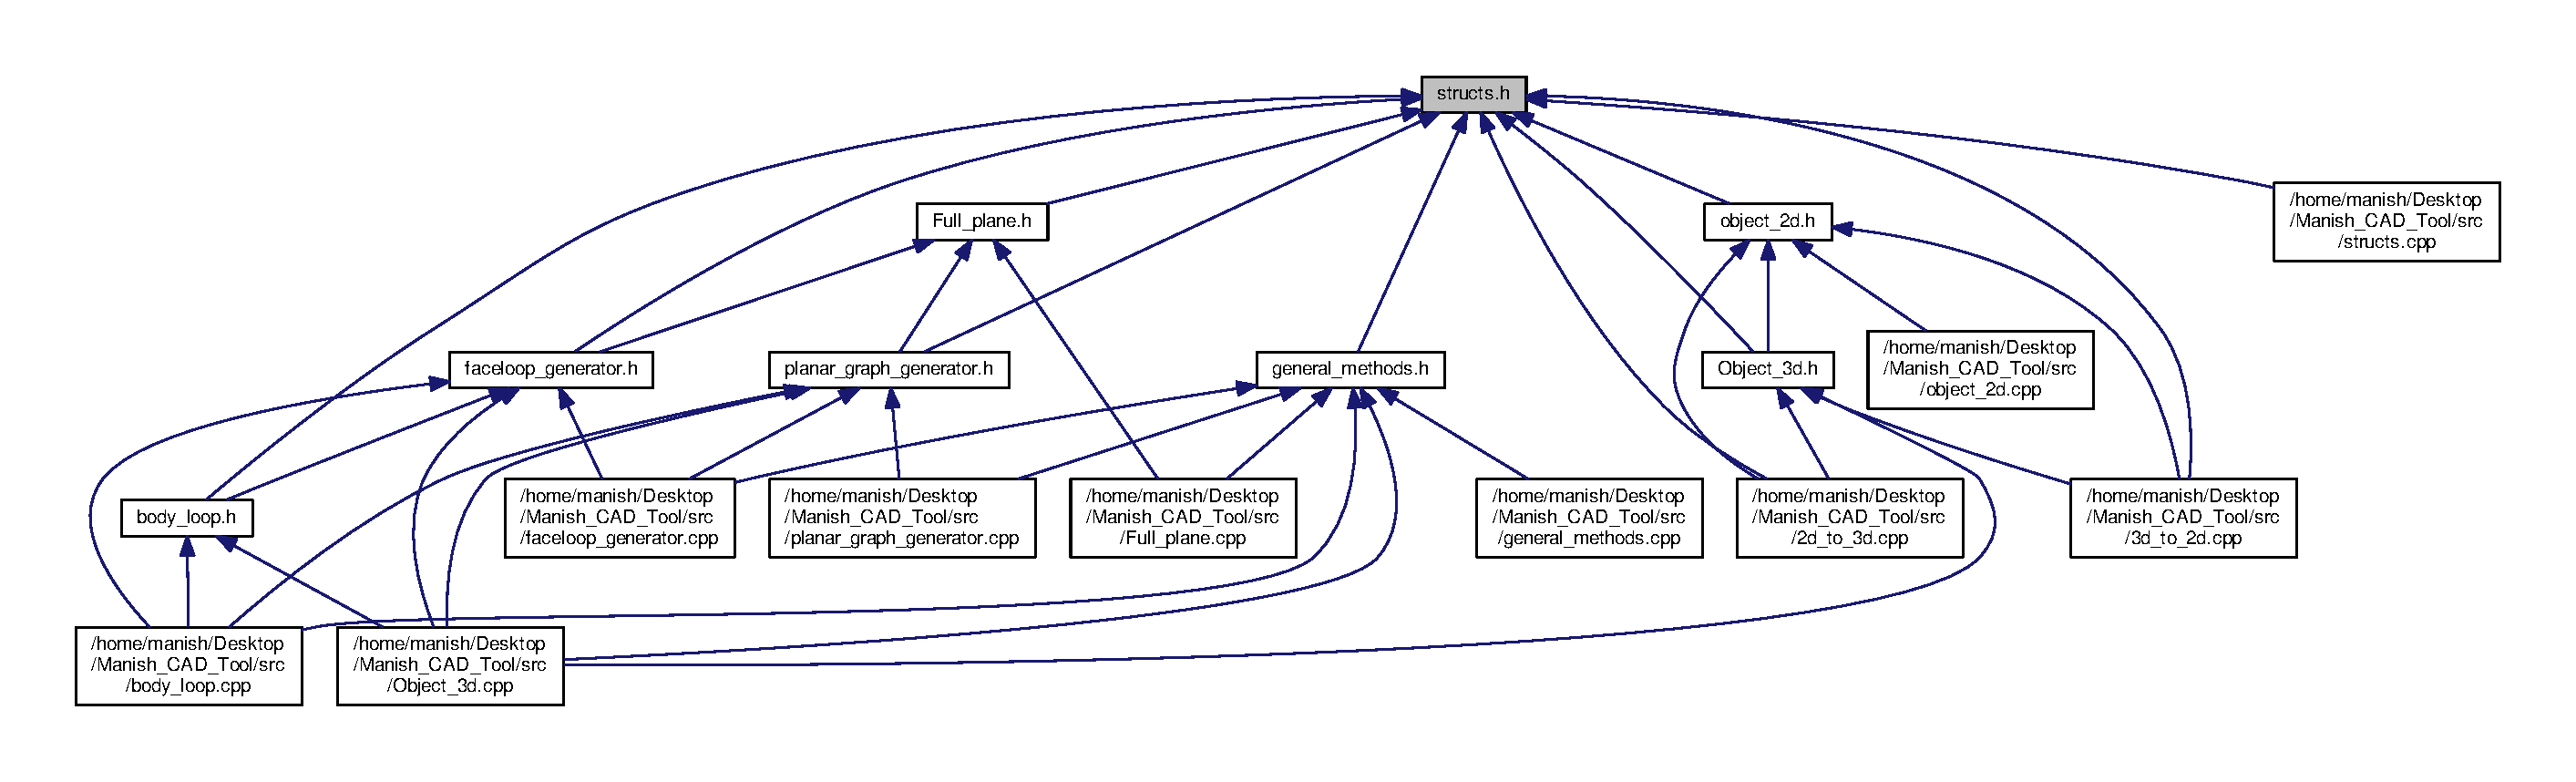
\includegraphics[width=350pt]{structs_8h__dep__incl}
\end{center}
\end{figure}
\subsection*{Classes}
\begin{DoxyCompactItemize}
\item 
class \hyperlink{classvertex__2d}{vertex\+\_\+2d}
\begin{DoxyCompactList}\small\item\em class for a \hyperlink{classvertex__2d}{vertex\+\_\+2d} \end{DoxyCompactList}\item 
class \hyperlink{classedge__2d}{edge\+\_\+2d}
\begin{DoxyCompactList}\small\item\em class for an \hyperlink{classedge__2d}{edge\+\_\+2d} \end{DoxyCompactList}\item 
class \hyperlink{classedge__2d__v2v}{edge\+\_\+2d\+\_\+v2v}
\begin{DoxyCompactList}\small\item\em class for an \hyperlink{classedge__2d__v2v}{edge\+\_\+2d\+\_\+v2v} \end{DoxyCompactList}\item 
class \hyperlink{classvertex__3d}{vertex\+\_\+3d}
\begin{DoxyCompactList}\small\item\em class for a \hyperlink{classvertex__3d}{vertex\+\_\+3d} \end{DoxyCompactList}\item 
class \hyperlink{classedge__3d}{edge\+\_\+3d}
\begin{DoxyCompactList}\small\item\em class for an \hyperlink{classedge__3d}{edge\+\_\+3d} \end{DoxyCompactList}\item 
class \hyperlink{classplane}{plane}
\begin{DoxyCompactList}\small\item\em class for a plane plane represented as (a,b,c,d) corresponding to the equation ax + by + cz = d \end{DoxyCompactList}\end{DoxyCompactItemize}
\subsection*{Macros}
\begin{DoxyCompactItemize}
\item 
\#define \hyperlink{structs_8h_a42257a545daf5b7933d6e8f96adc74f2}{F}~first
\item 
\#define \hyperlink{structs_8h_af933676109efed7ab34cea71d748a517}{S}~second
\item 
\#define \hyperlink{structs_8h_a276c5a0e984cf60015b27252fe04fe6b}{pb}~push\+\_\+back
\end{DoxyCompactItemize}


\subsection{Macro Definition Documentation}
\index{structs.\+h@{structs.\+h}!F@{F}}
\index{F@{F}!structs.\+h@{structs.\+h}}
\subsubsection[{\texorpdfstring{F}{F}}]{\setlength{\rightskip}{0pt plus 5cm}\#define F~first}\hypertarget{structs_8h_a42257a545daf5b7933d6e8f96adc74f2}{}\label{structs_8h_a42257a545daf5b7933d6e8f96adc74f2}


Definition at line 3 of file structs.\+h.

\index{structs.\+h@{structs.\+h}!pb@{pb}}
\index{pb@{pb}!structs.\+h@{structs.\+h}}
\subsubsection[{\texorpdfstring{pb}{pb}}]{\setlength{\rightskip}{0pt plus 5cm}\#define pb~push\+\_\+back}\hypertarget{structs_8h_a276c5a0e984cf60015b27252fe04fe6b}{}\label{structs_8h_a276c5a0e984cf60015b27252fe04fe6b}


Definition at line 5 of file structs.\+h.

\index{structs.\+h@{structs.\+h}!S@{S}}
\index{S@{S}!structs.\+h@{structs.\+h}}
\subsubsection[{\texorpdfstring{S}{S}}]{\setlength{\rightskip}{0pt plus 5cm}\#define S~second}\hypertarget{structs_8h_af933676109efed7ab34cea71d748a517}{}\label{structs_8h_af933676109efed7ab34cea71d748a517}


Definition at line 4 of file structs.\+h.


\hypertarget{2d__to__3d_8cpp}{}\section{/home/manish/\+Desktop/\+Manish\+\_\+\+C\+A\+D\+\_\+\+Tool/src/2d\+\_\+to\+\_\+3d.cpp File Reference}
\label{2d__to__3d_8cpp}\index{/home/manish/\+Desktop/\+Manish\+\_\+\+C\+A\+D\+\_\+\+Tool/src/2d\+\_\+to\+\_\+3d.\+cpp@{/home/manish/\+Desktop/\+Manish\+\_\+\+C\+A\+D\+\_\+\+Tool/src/2d\+\_\+to\+\_\+3d.\+cpp}}
{\ttfamily \#include \char`\"{}include/structs.\+h\char`\"{}}\\*
{\ttfamily \#include \char`\"{}include/object\+\_\+2d.\+h\char`\"{}}\\*
{\ttfamily \#include \char`\"{}include/\+Object\+\_\+3d.\+h\char`\"{}}\\*
{\ttfamily \#include \char`\"{}include/2d\+\_\+to\+\_\+3d.\+h\char`\"{}}\\*
{\ttfamily \#include \char`\"{}form.\+h\char`\"{}}\\*
{\ttfamily \#include $<$bits/stdc++.\+h$>$}\\*
{\ttfamily \#include $<$Q\+Widget$>$}\\*
Include dependency graph for 2d\+\_\+to\+\_\+3d.cpp\+:
\nopagebreak
\begin{figure}[H]
\begin{center}
\leavevmode
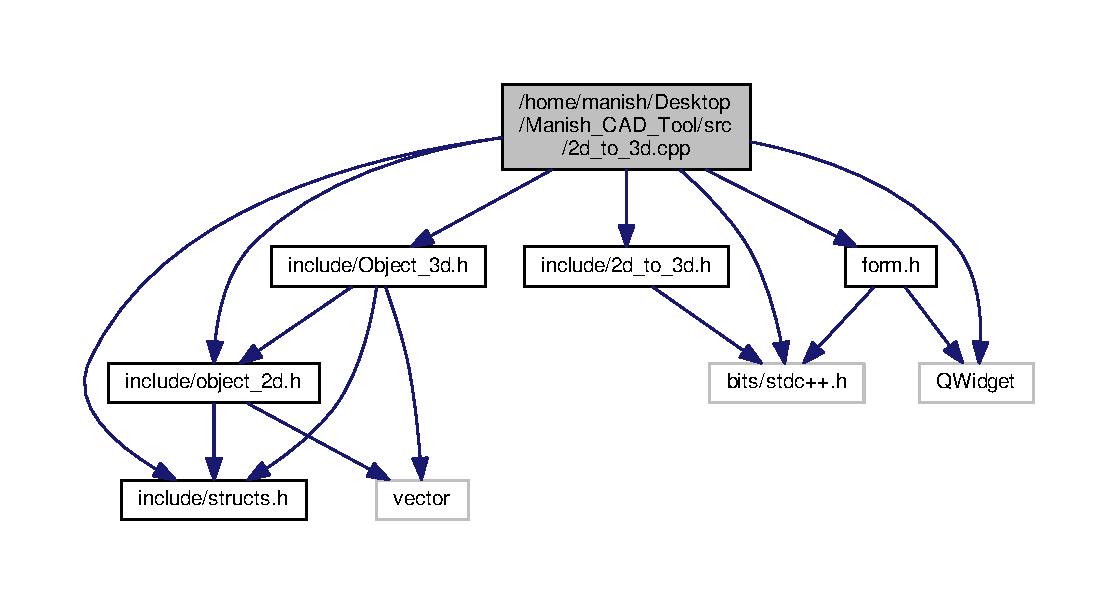
\includegraphics[width=350pt]{2d__to__3d_8cpp__incl}
\end{center}
\end{figure}
\subsection*{Functions}
\begin{DoxyCompactItemize}
\item 
int \hyperlink{2d__to__3d_8cpp_a46fa6b9417f38de819c57c2395143af6}{two\+\_\+d\+\_\+to\+\_\+three\+\_\+d} (string file, string outfile)
\end{DoxyCompactItemize}


\subsection{Function Documentation}
\index{2d\+\_\+to\+\_\+3d.\+cpp@{2d\+\_\+to\+\_\+3d.\+cpp}!two\+\_\+d\+\_\+to\+\_\+three\+\_\+d@{two\+\_\+d\+\_\+to\+\_\+three\+\_\+d}}
\index{two\+\_\+d\+\_\+to\+\_\+three\+\_\+d@{two\+\_\+d\+\_\+to\+\_\+three\+\_\+d}!2d\+\_\+to\+\_\+3d.\+cpp@{2d\+\_\+to\+\_\+3d.\+cpp}}
\subsubsection[{\texorpdfstring{two\+\_\+d\+\_\+to\+\_\+three\+\_\+d(string file, string outfile)}{two_d_to_three_d(string file, string outfile)}}]{\setlength{\rightskip}{0pt plus 5cm}int two\+\_\+d\+\_\+to\+\_\+three\+\_\+d (
\begin{DoxyParamCaption}
\item[{string}]{file, }
\item[{string}]{outfile}
\end{DoxyParamCaption}
)}\hypertarget{2d__to__3d_8cpp_a46fa6b9417f38de819c57c2395143af6}{}\label{2d__to__3d_8cpp_a46fa6b9417f38de819c57c2395143af6}
$<$ vector of co-\/ordinates of vertices in top-\/view

$<$ vector of co-\/ordinates of vertices in front-\/view

$<$ vector of co-\/ordinates of vertices in side-\/view

$<$ vector of edges in top-\/view

$<$ vector of edges in front-\/view

$<$ vector of edges in side-\/view 

Definition at line 14 of file 2d\+\_\+to\+\_\+3d.\+cpp.


\hypertarget{3d__to__2d_8cpp}{}\section{/home/manish/\+Desktop/\+Manish\+\_\+\+C\+A\+D\+\_\+\+Tool/src/3d\+\_\+to\+\_\+2d.cpp File Reference}
\label{3d__to__2d_8cpp}\index{/home/manish/\+Desktop/\+Manish\+\_\+\+C\+A\+D\+\_\+\+Tool/src/3d\+\_\+to\+\_\+2d.\+cpp@{/home/manish/\+Desktop/\+Manish\+\_\+\+C\+A\+D\+\_\+\+Tool/src/3d\+\_\+to\+\_\+2d.\+cpp}}
{\ttfamily \#include \char`\"{}include/structs.\+h\char`\"{}}\\*
{\ttfamily \#include \char`\"{}include/object\+\_\+2d.\+h\char`\"{}}\\*
{\ttfamily \#include \char`\"{}include/\+Object\+\_\+3d.\+h\char`\"{}}\\*
{\ttfamily \#include \char`\"{}include/3d\+\_\+to\+\_\+2d.\+h\char`\"{}}\\*
{\ttfamily \#include \char`\"{}include/form.\+h\char`\"{}}\\*
{\ttfamily \#include $<$bits/stdc++.\+h$>$}\\*
{\ttfamily \#include $<$Q\+Widget$>$}\\*
Include dependency graph for 3d\+\_\+to\+\_\+2d.cpp\+:
\nopagebreak
\begin{figure}[H]
\begin{center}
\leavevmode
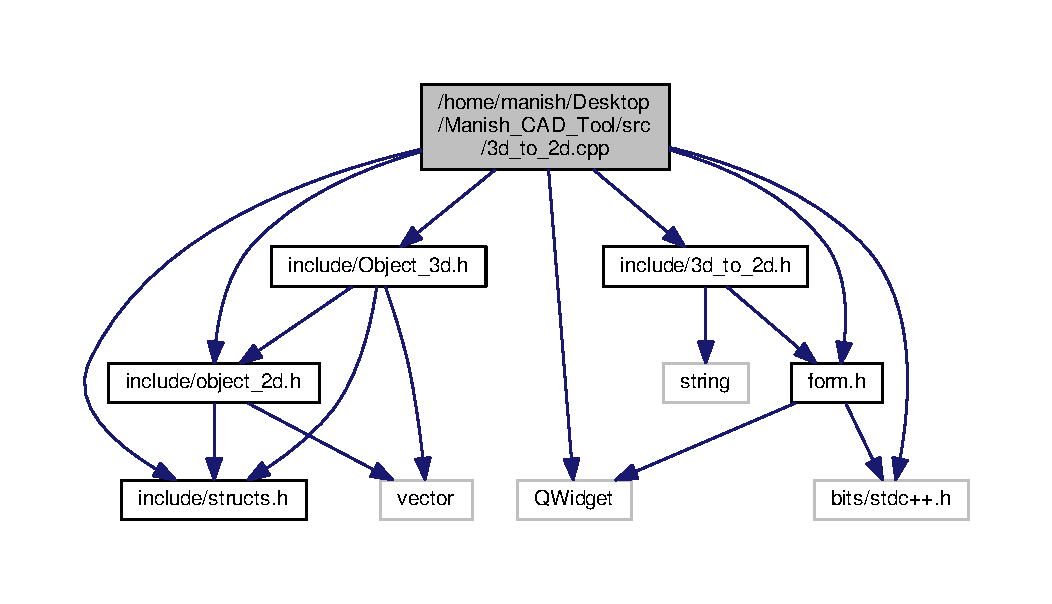
\includegraphics[width=350pt]{3d__to__2d_8cpp__incl}
\end{center}
\end{figure}
\subsection*{Functions}
\begin{DoxyCompactItemize}
\item 
int \hyperlink{3d__to__2d_8cpp_ab538d2702fd0abf46645a902ace3fe93}{three\+\_\+d\+\_\+to\+\_\+two\+\_\+d} (string file)
\end{DoxyCompactItemize}


\subsection{Function Documentation}
\index{3d\+\_\+to\+\_\+2d.\+cpp@{3d\+\_\+to\+\_\+2d.\+cpp}!three\+\_\+d\+\_\+to\+\_\+two\+\_\+d@{three\+\_\+d\+\_\+to\+\_\+two\+\_\+d}}
\index{three\+\_\+d\+\_\+to\+\_\+two\+\_\+d@{three\+\_\+d\+\_\+to\+\_\+two\+\_\+d}!3d\+\_\+to\+\_\+2d.\+cpp@{3d\+\_\+to\+\_\+2d.\+cpp}}
\subsubsection[{\texorpdfstring{three\+\_\+d\+\_\+to\+\_\+two\+\_\+d(string file)}{three_d_to_two_d(string file)}}]{\setlength{\rightskip}{0pt plus 5cm}int three\+\_\+d\+\_\+to\+\_\+two\+\_\+d (
\begin{DoxyParamCaption}
\item[{string}]{file}
\end{DoxyParamCaption}
)}\hypertarget{3d__to__2d_8cpp_ab538d2702fd0abf46645a902ace3fe93}{}\label{3d__to__2d_8cpp_ab538d2702fd0abf46645a902ace3fe93}


Definition at line 14 of file 3d\+\_\+to\+\_\+2d.\+cpp.


\hypertarget{body__loop_8cpp}{}\section{/home/manish/\+Desktop/\+Manish\+\_\+\+C\+A\+D\+\_\+\+Tool/src/body\+\_\+loop.cpp File Reference}
\label{body__loop_8cpp}\index{/home/manish/\+Desktop/\+Manish\+\_\+\+C\+A\+D\+\_\+\+Tool/src/body\+\_\+loop.\+cpp@{/home/manish/\+Desktop/\+Manish\+\_\+\+C\+A\+D\+\_\+\+Tool/src/body\+\_\+loop.\+cpp}}
{\ttfamily \#include \char`\"{}include/faceloop\+\_\+generator.\+h\char`\"{}}\\*
{\ttfamily \#include \char`\"{}include/general\+\_\+methods.\+h\char`\"{}}\\*
{\ttfamily \#include \char`\"{}include/planar\+\_\+graph\+\_\+generator.\+h\char`\"{}}\\*
{\ttfamily \#include \char`\"{}include/body\+\_\+loop.\+h\char`\"{}}\\*
{\ttfamily \#include $<$cmath$>$}\\*
{\ttfamily \#include $<$algorithm$>$}\\*
{\ttfamily \#include $<$iostream$>$}\\*
{\ttfamily \#include $<$map$>$}\\*
Include dependency graph for body\+\_\+loop.\+cpp\+:
\nopagebreak
\begin{figure}[H]
\begin{center}
\leavevmode
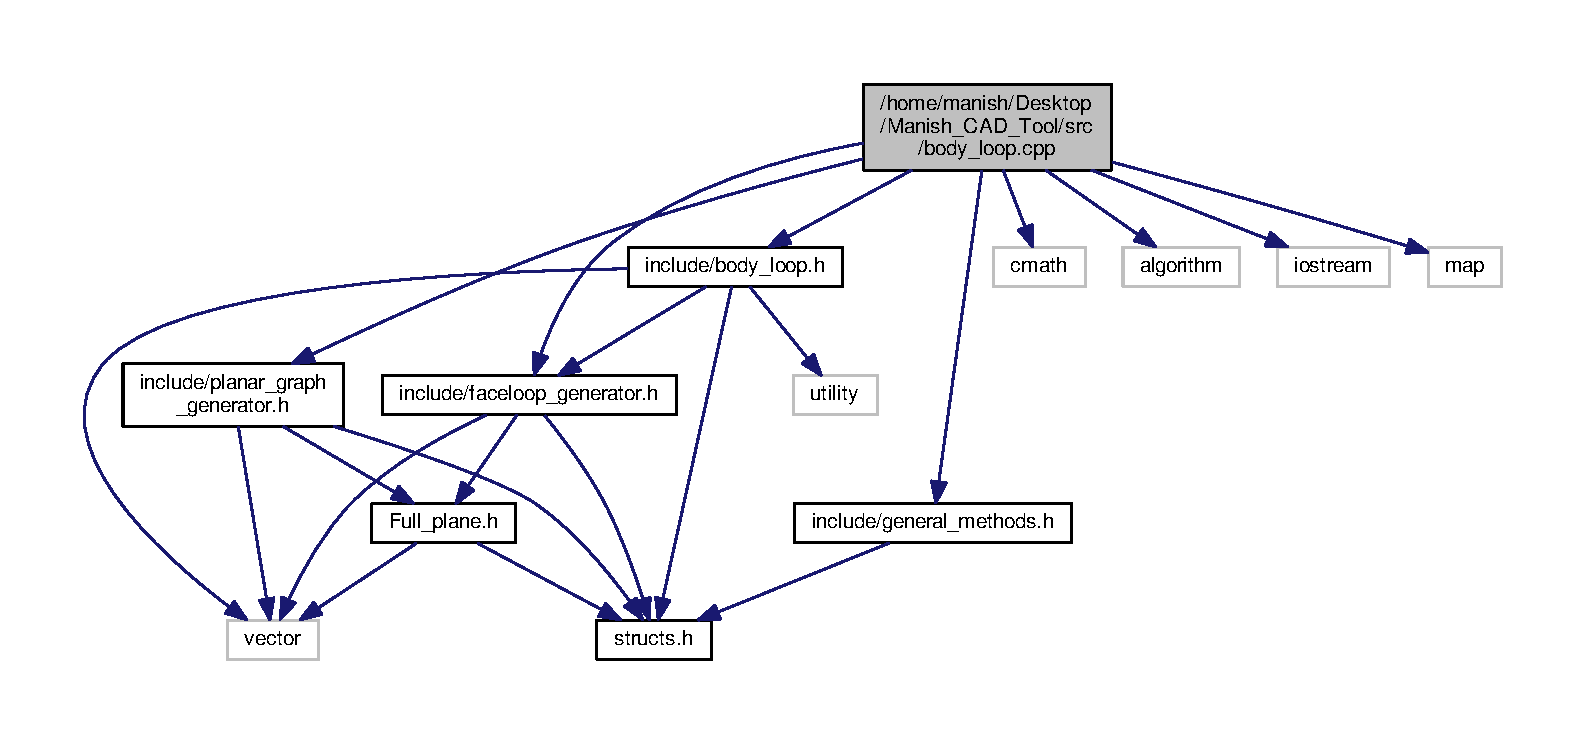
\includegraphics[width=350pt]{body__loop_8cpp__incl}
\end{center}
\end{figure}
\subsection*{Macros}
\begin{DoxyCompactItemize}
\item 
\#define \hyperlink{body__loop_8cpp_a71064b70dc7b2e65c2aa8a0555cf2efd}{epsil}~0.\+000001
\item 
\#define \hyperlink{body__loop_8cpp_a598a3330b3c21701223ee0ca14316eca}{PI}~3.\+14159265
\end{DoxyCompactItemize}
\subsection*{Functions}
\begin{DoxyCompactItemize}
\item 
std\+::vector$<$ \hyperlink{classbody__loop}{body\+\_\+loop} $>$ \hyperlink{body__loop_8cpp_a230720d5c9d1a2805c6c743287d28d5b}{generate\+\_\+body\+\_\+loop} (std\+::vector$<$ \hyperlink{classface__loop}{face\+\_\+loop} $>$ face\+\_\+loop\+\_\+list, std\+::vector$<$ \hyperlink{classvertex__3d}{vertex\+\_\+3d} $>$ v3d\+\_\+list)
\item 
pair$<$ int, bool $>$ \hyperlink{body__loop_8cpp_a85f5918713a8c62784797c5766195628}{successive\+\_\+face\+\_\+loop} (std\+::vector$<$ \hyperlink{classface__loop}{face\+\_\+loop} $>$ face\+\_\+loop\+\_\+list, \hyperlink{classface__loop}{face\+\_\+loop} fl, int fl\+\_\+int, bool side, \hyperlink{classedge__3d}{edge\+\_\+3d} e, std\+::vector$<$ \hyperlink{classvertex__3d}{vertex\+\_\+3d} $>$ v3d\+\_\+list, bool inner\+\_\+basic)
\item 
void \hyperlink{body__loop_8cpp_af9a0c6603771f19b48cb31a570811386}{initialize\+\_\+side\+\_\+used} (std\+::vector$<$ pair$<$ bool, bool $>$ $>$ \&side\+\_\+used)
\begin{DoxyCompactList}\small\item\em function that initializes side\+\_\+used for both sides + and -\/ for every body loop \end{DoxyCompactList}\item 
bool \hyperlink{body__loop_8cpp_aad211473d1c05d9bfce31774964bbd9a}{check\+\_\+legality} (\hyperlink{classbody__loop}{body\+\_\+loop} bl)
\begin{DoxyCompactList}\small\item\em function that checks that if a body part generated is legal or not \end{DoxyCompactList}\item 
bool \hyperlink{body__loop_8cpp_a68ebe3fd8487bbca7800bd67b4386970}{inner\+\_\+outer} (\hyperlink{classbody__loop}{body\+\_\+loop} bp, std\+::vector$<$ \hyperlink{classvertex__3d}{vertex\+\_\+3d} $>$ v3d\+\_\+list)
\begin{DoxyCompactList}\small\item\em function that determines if give body loop is inner or outer \end{DoxyCompactList}\item 
std\+::vector$<$ float $>$ \hyperlink{body__loop_8cpp_ad8e1589cd5ef438b41ebcce9fc970049}{get\+\_\+ray\+\_\+l} (\hyperlink{classplane}{plane} p1, \hyperlink{classplane}{plane} p2, bool s1, bool s2)
\begin{DoxyCompactList}\small\item\em function that determines vector along ray l = /$\vert$n1$\vert$ + /$\vert$n2$\vert$, where @ is the corresponding side \end{DoxyCompactList}\end{DoxyCompactItemize}


\subsection{Macro Definition Documentation}
\index{body\+\_\+loop.\+cpp@{body\+\_\+loop.\+cpp}!epsil@{epsil}}
\index{epsil@{epsil}!body\+\_\+loop.\+cpp@{body\+\_\+loop.\+cpp}}
\subsubsection[{\texorpdfstring{epsil}{epsil}}]{\setlength{\rightskip}{0pt plus 5cm}\#define epsil~0.\+000001}\hypertarget{body__loop_8cpp_a71064b70dc7b2e65c2aa8a0555cf2efd}{}\label{body__loop_8cpp_a71064b70dc7b2e65c2aa8a0555cf2efd}


Definition at line 6 of file body\+\_\+loop.\+cpp.

\index{body\+\_\+loop.\+cpp@{body\+\_\+loop.\+cpp}!PI@{PI}}
\index{PI@{PI}!body\+\_\+loop.\+cpp@{body\+\_\+loop.\+cpp}}
\subsubsection[{\texorpdfstring{PI}{PI}}]{\setlength{\rightskip}{0pt plus 5cm}\#define PI~3.\+14159265}\hypertarget{body__loop_8cpp_a598a3330b3c21701223ee0ca14316eca}{}\label{body__loop_8cpp_a598a3330b3c21701223ee0ca14316eca}


Definition at line 7 of file body\+\_\+loop.\+cpp.



\subsection{Function Documentation}
\index{body\+\_\+loop.\+cpp@{body\+\_\+loop.\+cpp}!check\+\_\+legality@{check\+\_\+legality}}
\index{check\+\_\+legality@{check\+\_\+legality}!body\+\_\+loop.\+cpp@{body\+\_\+loop.\+cpp}}
\subsubsection[{\texorpdfstring{check\+\_\+legality(body\+\_\+loop bl)}{check_legality(body_loop bl)}}]{\setlength{\rightskip}{0pt plus 5cm}bool check\+\_\+legality (
\begin{DoxyParamCaption}
\item[{{\bf body\+\_\+loop}}]{bl}
\end{DoxyParamCaption}
)}\hypertarget{body__loop_8cpp_aad211473d1c05d9bfce31774964bbd9a}{}\label{body__loop_8cpp_aad211473d1c05d9bfce31774964bbd9a}


function that checks that if a body part generated is legal or not 



Definition at line 160 of file body\+\_\+loop.\+cpp.

\index{body\+\_\+loop.\+cpp@{body\+\_\+loop.\+cpp}!generate\+\_\+body\+\_\+loop@{generate\+\_\+body\+\_\+loop}}
\index{generate\+\_\+body\+\_\+loop@{generate\+\_\+body\+\_\+loop}!body\+\_\+loop.\+cpp@{body\+\_\+loop.\+cpp}}
\subsubsection[{\texorpdfstring{generate\+\_\+body\+\_\+loop(std\+::vector$<$ face\+\_\+loop $>$ face\+\_\+loop\+\_\+list, std\+::vector$<$ vertex\+\_\+3d $>$ v3d\+\_\+list)}{generate_body_loop(std::vector< face_loop > face_loop_list, std::vector< vertex_3d > v3d_list)}}]{\setlength{\rightskip}{0pt plus 5cm}std\+::vector$<$ {\bf body\+\_\+loop} $>$ generate\+\_\+body\+\_\+loop (
\begin{DoxyParamCaption}
\item[{std\+::vector$<$ {\bf face\+\_\+loop} $>$}]{face\+\_\+loop\+\_\+list, }
\item[{std\+::vector$<$ {\bf vertex\+\_\+3d} $>$}]{v3d\+\_\+list}
\end{DoxyParamCaption}
)}\hypertarget{body__loop_8cpp_a230720d5c9d1a2805c6c743287d28d5b}{}\label{body__loop_8cpp_a230720d5c9d1a2805c6c743287d28d5b}

\begin{DoxyParams}{Parameters}
{\em face\+\_\+loop\+\_\+list} & list of all face loops generated for the reconstruction \\
\hline
{\em v3d\+\_\+list} & vector of the 3d-\/vertices of the 3D object \\
\hline
\end{DoxyParams}


Definition at line 33 of file body\+\_\+loop.\+cpp.

\index{body\+\_\+loop.\+cpp@{body\+\_\+loop.\+cpp}!get\+\_\+ray\+\_\+l@{get\+\_\+ray\+\_\+l}}
\index{get\+\_\+ray\+\_\+l@{get\+\_\+ray\+\_\+l}!body\+\_\+loop.\+cpp@{body\+\_\+loop.\+cpp}}
\subsubsection[{\texorpdfstring{get\+\_\+ray\+\_\+l(plane p1, plane p2, bool s1, bool s2)}{get_ray_l(plane p1, plane p2, bool s1, bool s2)}}]{\setlength{\rightskip}{0pt plus 5cm}std\+::vector$<$float$>$ get\+\_\+ray\+\_\+l (
\begin{DoxyParamCaption}
\item[{{\bf plane}}]{p1, }
\item[{{\bf plane}}]{p2, }
\item[{bool}]{s1, }
\item[{bool}]{s2}
\end{DoxyParamCaption}
)}\hypertarget{body__loop_8cpp_ad8e1589cd5ef438b41ebcce9fc970049}{}\label{body__loop_8cpp_ad8e1589cd5ef438b41ebcce9fc970049}


function that determines vector along ray l = /$\vert$n1$\vert$ + /$\vert$n2$\vert$, where @ is the corresponding side 



Definition at line 187 of file body\+\_\+loop.\+cpp.

\index{body\+\_\+loop.\+cpp@{body\+\_\+loop.\+cpp}!initialize\+\_\+side\+\_\+used@{initialize\+\_\+side\+\_\+used}}
\index{initialize\+\_\+side\+\_\+used@{initialize\+\_\+side\+\_\+used}!body\+\_\+loop.\+cpp@{body\+\_\+loop.\+cpp}}
\subsubsection[{\texorpdfstring{initialize\+\_\+side\+\_\+used(std\+::vector$<$ pair$<$ bool, bool $>$ $>$ \&side\+\_\+used)}{initialize_side_used(std::vector< pair< bool, bool > > &side_used)}}]{\setlength{\rightskip}{0pt plus 5cm}void initialize\+\_\+side\+\_\+used (
\begin{DoxyParamCaption}
\item[{std\+::vector$<$ pair$<$ bool, bool $>$ $>$ \&}]{side\+\_\+used}
\end{DoxyParamCaption}
)}\hypertarget{body__loop_8cpp_af9a0c6603771f19b48cb31a570811386}{}\label{body__loop_8cpp_af9a0c6603771f19b48cb31a570811386}


function that initializes side\+\_\+used for both sides + and -\/ for every body loop 



Definition at line 152 of file body\+\_\+loop.\+cpp.

\index{body\+\_\+loop.\+cpp@{body\+\_\+loop.\+cpp}!inner\+\_\+outer@{inner\+\_\+outer}}
\index{inner\+\_\+outer@{inner\+\_\+outer}!body\+\_\+loop.\+cpp@{body\+\_\+loop.\+cpp}}
\subsubsection[{\texorpdfstring{inner\+\_\+outer(body\+\_\+loop bp, std\+::vector$<$ vertex\+\_\+3d $>$ v3d\+\_\+list)}{inner_outer(body_loop bp, std::vector< vertex_3d > v3d_list)}}]{\setlength{\rightskip}{0pt plus 5cm}bool inner\+\_\+outer (
\begin{DoxyParamCaption}
\item[{{\bf body\+\_\+loop}}]{bp, }
\item[{std\+::vector$<$ {\bf vertex\+\_\+3d} $>$}]{v3d\+\_\+list}
\end{DoxyParamCaption}
)}\hypertarget{body__loop_8cpp_a68ebe3fd8487bbca7800bd67b4386970}{}\label{body__loop_8cpp_a68ebe3fd8487bbca7800bd67b4386970}


function that determines if give body loop is inner or outer 



Definition at line 180 of file body\+\_\+loop.\+cpp.

\index{body\+\_\+loop.\+cpp@{body\+\_\+loop.\+cpp}!successive\+\_\+face\+\_\+loop@{successive\+\_\+face\+\_\+loop}}
\index{successive\+\_\+face\+\_\+loop@{successive\+\_\+face\+\_\+loop}!body\+\_\+loop.\+cpp@{body\+\_\+loop.\+cpp}}
\subsubsection[{\texorpdfstring{successive\+\_\+face\+\_\+loop(std\+::vector$<$ face\+\_\+loop $>$ face\+\_\+loop\+\_\+list, face\+\_\+loop fl, int fl\+\_\+int, bool side, edge\+\_\+3d e, std\+::vector$<$ vertex\+\_\+3d $>$ v3d\+\_\+list, bool inner\+\_\+basic)}{successive_face_loop(std::vector< face_loop > face_loop_list, face_loop fl, int fl_int, bool side, edge_3d e, std::vector< vertex_3d > v3d_list, bool inner_basic)}}]{\setlength{\rightskip}{0pt plus 5cm}pair$<$int,bool$>$ successive\+\_\+face\+\_\+loop (
\begin{DoxyParamCaption}
\item[{std\+::vector$<$ {\bf face\+\_\+loop} $>$}]{face\+\_\+loop\+\_\+list, }
\item[{{\bf face\+\_\+loop}}]{fl, }
\item[{int}]{fl\+\_\+int, }
\item[{bool}]{side, }
\item[{{\bf edge\+\_\+3d}}]{e, }
\item[{std\+::vector$<$ {\bf vertex\+\_\+3d} $>$}]{v3d\+\_\+list, }
\item[{bool}]{inner\+\_\+basic}
\end{DoxyParamCaption}
)}\hypertarget{body__loop_8cpp_a85f5918713a8c62784797c5766195628}{}\label{body__loop_8cpp_a85f5918713a8c62784797c5766195628}

\begin{DoxyParams}{Parameters}
{\em face\+\_\+loop\+\_\+list} & list of all face loops of the object \\
\hline
{\em fl} & face loop for which successive face loop is being found \\
\hline
{\em side} & side of the face loop (i.\+e + or -\/) \\
\hline
{\em e} & edge of the face loop fl at which successive face loop has to be found \\
\hline
{\em e\+\_\+vector} & 3$\ast$1 vector for direction of the edge e \\
\hline
\end{DoxyParams}
\begin{DoxyReturn}{Returns}
the index of successive face loop and its side 
\end{DoxyReturn}


Definition at line 111 of file body\+\_\+loop.\+cpp.


\hypertarget{faceloop__generator_8cpp}{}\section{/home/manish/\+Desktop/\+Manish\+\_\+\+C\+A\+D\+\_\+\+Tool/src/faceloop\+\_\+generator.cpp File Reference}
\label{faceloop__generator_8cpp}\index{/home/manish/\+Desktop/\+Manish\+\_\+\+C\+A\+D\+\_\+\+Tool/src/faceloop\+\_\+generator.\+cpp@{/home/manish/\+Desktop/\+Manish\+\_\+\+C\+A\+D\+\_\+\+Tool/src/faceloop\+\_\+generator.\+cpp}}
{\ttfamily \#include \char`\"{}include/faceloop\+\_\+generator.\+h\char`\"{}}\\*
{\ttfamily \#include \char`\"{}include/general\+\_\+methods.\+h\char`\"{}}\\*
{\ttfamily \#include \char`\"{}include/planar\+\_\+graph\+\_\+generator.\+h\char`\"{}}\\*
{\ttfamily \#include $<$cmath$>$}\\*
{\ttfamily \#include $<$algorithm$>$}\\*
{\ttfamily \#include $<$iostream$>$}\\*
Include dependency graph for faceloop\+\_\+generator.\+cpp\+:
\nopagebreak
\begin{figure}[H]
\begin{center}
\leavevmode
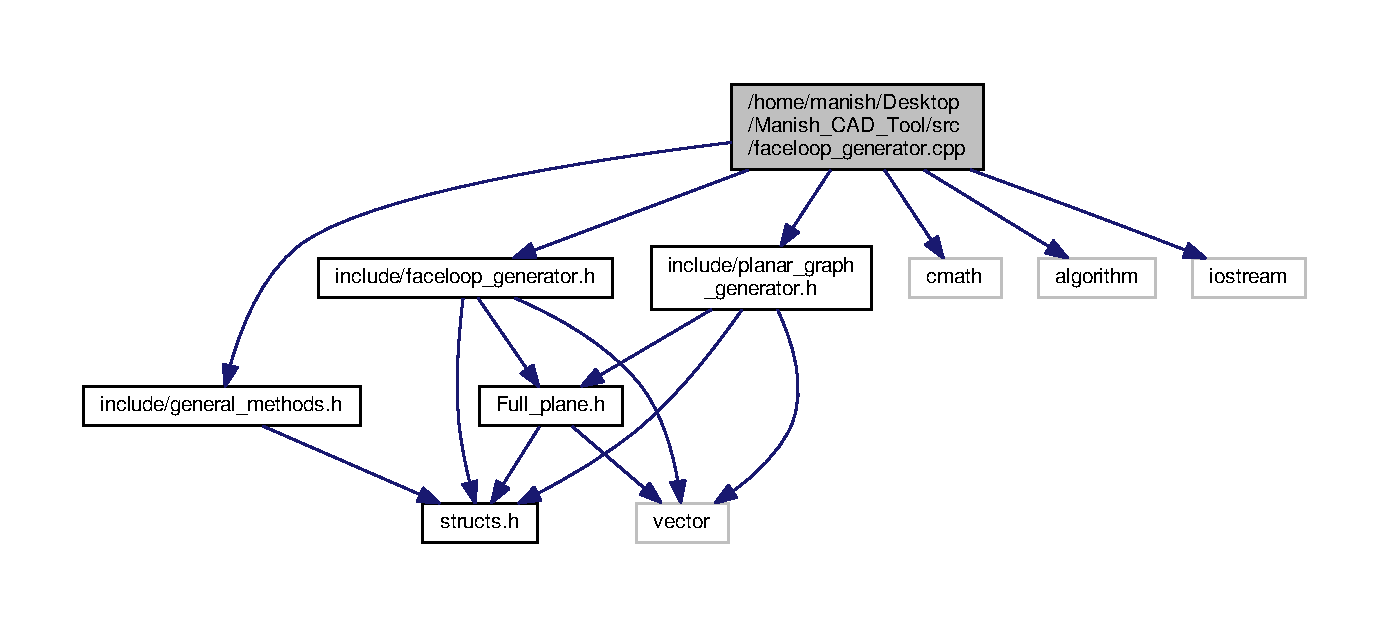
\includegraphics[width=350pt]{faceloop__generator_8cpp__incl}
\end{center}
\end{figure}
\subsection*{Macros}
\begin{DoxyCompactItemize}
\item 
\#define \hyperlink{faceloop__generator_8cpp_a71064b70dc7b2e65c2aa8a0555cf2efd}{epsil}~0.\+000001
\end{DoxyCompactItemize}
\subsection*{Functions}
\begin{DoxyCompactItemize}
\item 
std\+::vector$<$ \hyperlink{classface__loop}{face\+\_\+loop} $>$ \hyperlink{faceloop__generator_8cpp_ae6b709b480a42b239420e2f968bf4a6c}{generate\+\_\+face\+\_\+loops} (\hyperlink{classplane}{plane} p, std\+::vector$<$ int $>$ vertices\+\_\+on\+\_\+the\+\_\+plane, std\+::vector$<$ \hyperlink{classedge__3d}{edge\+\_\+3d} $>$ \&edges\+\_\+on\+\_\+the\+\_\+plane, std\+::vector$<$ \hyperlink{classvertex__3d}{vertex\+\_\+3d} $>$ v3d\+\_\+list)
\item 
bool \hyperlink{faceloop__generator_8cpp_a67ea41ab7b651bc5783a4a43a9e1eaea}{compare\+\_\+angles} (std\+::pair$<$ int, std\+::pair$<$ float, bool $>$ $>$ lhs, std\+::pair$<$ int, std\+::pair$<$ float, bool $>$ $>$ rhs)
\item 
void \hyperlink{faceloop__generator_8cpp_a0e4704601381cabb530aa622af4b55d0}{sort\+\_\+edges} (std\+::vector$<$ int $>$ \&v, int i, std\+::vector$<$ \hyperlink{classvertex__3d}{vertex\+\_\+3d} $>$ v3d\+\_\+list)
\item 
std\+::vector$<$ std\+::vector$<$ int $>$ $>$ \hyperlink{faceloop__generator_8cpp_aadb442650ebd831d3c7fda4a627d1ace}{generate\+\_\+ordered\+\_\+adj\+\_\+list} (std\+::vector$<$ \hyperlink{classedge__3d}{edge\+\_\+3d} $>$ edges\+\_\+on\+\_\+the\+\_\+plane, std\+::vector$<$ int $>$ vertices\+\_\+on\+\_\+the\+\_\+plane, std\+::vector$<$ \hyperlink{classvertex__3d}{vertex\+\_\+3d} $>$ v3d\+\_\+list)
\begin{DoxyCompactList}\small\item\em function to generate ordered adj\+\_\+list in clockwise direction \end{DoxyCompactList}\item 
std\+::vector$<$ \hyperlink{classbasic__loop}{basic\+\_\+loop} $>$ \hyperlink{faceloop__generator_8cpp_a7a4a04f233606e5f06164dc9a97b47a5}{basic\+\_\+loop\+\_\+generator} (std\+::vector$<$ \hyperlink{classedge__3d}{edge\+\_\+3d} $>$ \&edges\+\_\+on\+\_\+the\+\_\+plane, std\+::vector$<$ vector$<$ int $>$ $>$ ordered\+\_\+adj\+\_\+list)
\begin{DoxyCompactList}\small\item\em function that generates basic loops \end{DoxyCompactList}\item 
bool \hyperlink{faceloop__generator_8cpp_a00972a0826ec9a1e09355a4d7085b06b}{is\+\_\+in\+\_\+it} (\hyperlink{classvertex__3d}{vertex\+\_\+3d} v1, \hyperlink{classbasic__loop}{basic\+\_\+loop} b, std\+::vector$<$ \hyperlink{classvertex__3d}{vertex\+\_\+3d} $>$ v3d\+\_\+list)
\item 
bool \hyperlink{faceloop__generator_8cpp_afa2e3a07821dc9581a2368710a15211c}{included} (\hyperlink{classbasic__loop}{basic\+\_\+loop} b1, \hyperlink{classbasic__loop}{basic\+\_\+loop} b2, std\+::vector$<$ \hyperlink{classvertex__3d}{vertex\+\_\+3d} $>$ v3d\+\_\+list)
\item 
std\+::vector$<$ std\+::vector$<$ bool $>$ $>$ \hyperlink{faceloop__generator_8cpp_a9a32da1f4ab031ab685165a2ac99dab8}{generate\+\_\+inclusion\+\_\+matrix} (std\+::vector$<$ \hyperlink{classbasic__loop}{basic\+\_\+loop} $>$ basic\+\_\+loop\+\_\+list, std\+::vector$<$ \hyperlink{classvertex__3d}{vertex\+\_\+3d} $>$ v3d\+\_\+list)
\begin{DoxyCompactList}\small\item\em function to generate inclusion matrix \end{DoxyCompactList}\end{DoxyCompactItemize}


\subsection{Macro Definition Documentation}
\index{faceloop\+\_\+generator.\+cpp@{faceloop\+\_\+generator.\+cpp}!epsil@{epsil}}
\index{epsil@{epsil}!faceloop\+\_\+generator.\+cpp@{faceloop\+\_\+generator.\+cpp}}
\subsubsection[{\texorpdfstring{epsil}{epsil}}]{\setlength{\rightskip}{0pt plus 5cm}\#define epsil~0.\+000001}\hypertarget{faceloop__generator_8cpp_a71064b70dc7b2e65c2aa8a0555cf2efd}{}\label{faceloop__generator_8cpp_a71064b70dc7b2e65c2aa8a0555cf2efd}


Definition at line 4 of file faceloop\+\_\+generator.\+cpp.



\subsection{Function Documentation}
\index{faceloop\+\_\+generator.\+cpp@{faceloop\+\_\+generator.\+cpp}!basic\+\_\+loop\+\_\+generator@{basic\+\_\+loop\+\_\+generator}}
\index{basic\+\_\+loop\+\_\+generator@{basic\+\_\+loop\+\_\+generator}!faceloop\+\_\+generator.\+cpp@{faceloop\+\_\+generator.\+cpp}}
\subsubsection[{\texorpdfstring{basic\+\_\+loop\+\_\+generator(std\+::vector$<$ edge\+\_\+3d $>$ \&edges\+\_\+on\+\_\+the\+\_\+plane, std\+::vector$<$ vector$<$ int $>$ $>$ ordered\+\_\+adj\+\_\+list)}{basic_loop_generator(std::vector< edge_3d > &edges_on_the_plane, std::vector< vector< int > > ordered_adj_list)}}]{\setlength{\rightskip}{0pt plus 5cm}std\+::vector$<$ {\bf basic\+\_\+loop} $>$ basic\+\_\+loop\+\_\+generator (
\begin{DoxyParamCaption}
\item[{std\+::vector$<$ {\bf edge\+\_\+3d} $>$ \&}]{edges\+\_\+on\+\_\+the\+\_\+plane, }
\item[{std\+::vector$<$ vector$<$ int $>$ $>$}]{ordered\+\_\+adj\+\_\+list}
\end{DoxyParamCaption}
)}\hypertarget{faceloop__generator_8cpp_a7a4a04f233606e5f06164dc9a97b47a5}{}\label{faceloop__generator_8cpp_a7a4a04f233606e5f06164dc9a97b47a5}


function that generates basic loops 



Definition at line 168 of file faceloop\+\_\+generator.\+cpp.

\index{faceloop\+\_\+generator.\+cpp@{faceloop\+\_\+generator.\+cpp}!compare\+\_\+angles@{compare\+\_\+angles}}
\index{compare\+\_\+angles@{compare\+\_\+angles}!faceloop\+\_\+generator.\+cpp@{faceloop\+\_\+generator.\+cpp}}
\subsubsection[{\texorpdfstring{compare\+\_\+angles(std\+::pair$<$ int, std\+::pair$<$ float, bool $>$ $>$ lhs, std\+::pair$<$ int, std\+::pair$<$ float, bool $>$ $>$ rhs)}{compare_angles(std::pair< int, std::pair< float, bool > > lhs, std::pair< int, std::pair< float, bool > > rhs)}}]{\setlength{\rightskip}{0pt plus 5cm}bool compare\+\_\+angles (
\begin{DoxyParamCaption}
\item[{std\+::pair$<$ int, std\+::pair$<$ float, bool $>$ $>$}]{lhs, }
\item[{std\+::pair$<$ int, std\+::pair$<$ float, bool $>$ $>$}]{rhs}
\end{DoxyParamCaption}
)}\hypertarget{faceloop__generator_8cpp_a67ea41ab7b651bc5783a4a43a9e1eaea}{}\label{faceloop__generator_8cpp_a67ea41ab7b651bc5783a4a43a9e1eaea}


Definition at line 111 of file faceloop\+\_\+generator.\+cpp.

\index{faceloop\+\_\+generator.\+cpp@{faceloop\+\_\+generator.\+cpp}!generate\+\_\+face\+\_\+loops@{generate\+\_\+face\+\_\+loops}}
\index{generate\+\_\+face\+\_\+loops@{generate\+\_\+face\+\_\+loops}!faceloop\+\_\+generator.\+cpp@{faceloop\+\_\+generator.\+cpp}}
\subsubsection[{\texorpdfstring{generate\+\_\+face\+\_\+loops(plane p, std\+::vector$<$ int $>$ vertices\+\_\+on\+\_\+the\+\_\+plane, std\+::vector$<$ edge\+\_\+3d $>$ \&edges\+\_\+on\+\_\+the\+\_\+plane, std\+::vector$<$ vertex\+\_\+3d $>$ v3d\+\_\+list)}{generate_face_loops(plane p, std::vector< int > vertices_on_the_plane, std::vector< edge_3d > &edges_on_the_plane, std::vector< vertex_3d > v3d_list)}}]{\setlength{\rightskip}{0pt plus 5cm}std\+::vector$<$ {\bf face\+\_\+loop} $>$ generate\+\_\+face\+\_\+loops (
\begin{DoxyParamCaption}
\item[{{\bf plane}}]{p, }
\item[{std\+::vector$<$ int $>$}]{vertices\+\_\+on\+\_\+the\+\_\+plane, }
\item[{std\+::vector$<$ {\bf edge\+\_\+3d} $>$ \&}]{edges\+\_\+on\+\_\+the\+\_\+plane, }
\item[{std\+::vector$<$ {\bf vertex\+\_\+3d} $>$}]{v3d\+\_\+list}
\end{DoxyParamCaption}
)}\hypertarget{faceloop__generator_8cpp_ae6b709b480a42b239420e2f968bf4a6c}{}\label{faceloop__generator_8cpp_ae6b709b480a42b239420e2f968bf4a6c}

\begin{DoxyParams}{Parameters}
{\em p} & plane for which face\+\_\+loops are being calculated \\
\hline
{\em edges\+\_\+on\+\_\+the\+\_\+plane} & vector of the edges which are on this plane \\
\hline
{\em v3d\+\_\+list} & vertex list of the 3d object \\
\hline
\end{DoxyParams}


Definition at line 36 of file faceloop\+\_\+generator.\+cpp.

\index{faceloop\+\_\+generator.\+cpp@{faceloop\+\_\+generator.\+cpp}!generate\+\_\+inclusion\+\_\+matrix@{generate\+\_\+inclusion\+\_\+matrix}}
\index{generate\+\_\+inclusion\+\_\+matrix@{generate\+\_\+inclusion\+\_\+matrix}!faceloop\+\_\+generator.\+cpp@{faceloop\+\_\+generator.\+cpp}}
\subsubsection[{\texorpdfstring{generate\+\_\+inclusion\+\_\+matrix(std\+::vector$<$ basic\+\_\+loop $>$ basic\+\_\+loop\+\_\+list, std\+::vector$<$ vertex\+\_\+3d $>$ v3d\+\_\+list)}{generate_inclusion_matrix(std::vector< basic_loop > basic_loop_list, std::vector< vertex_3d > v3d_list)}}]{\setlength{\rightskip}{0pt plus 5cm}std\+::vector$<$ std\+::vector$<$bool$>$ $>$ generate\+\_\+inclusion\+\_\+matrix (
\begin{DoxyParamCaption}
\item[{std\+::vector$<$ {\bf basic\+\_\+loop} $>$}]{basic\+\_\+loop\+\_\+list, }
\item[{std\+::vector$<$ {\bf vertex\+\_\+3d} $>$}]{v3d\+\_\+list}
\end{DoxyParamCaption}
)}\hypertarget{faceloop__generator_8cpp_a9a32da1f4ab031ab685165a2ac99dab8}{}\label{faceloop__generator_8cpp_a9a32da1f4ab031ab685165a2ac99dab8}


function to generate inclusion matrix 



Definition at line 392 of file faceloop\+\_\+generator.\+cpp.

\index{faceloop\+\_\+generator.\+cpp@{faceloop\+\_\+generator.\+cpp}!generate\+\_\+ordered\+\_\+adj\+\_\+list@{generate\+\_\+ordered\+\_\+adj\+\_\+list}}
\index{generate\+\_\+ordered\+\_\+adj\+\_\+list@{generate\+\_\+ordered\+\_\+adj\+\_\+list}!faceloop\+\_\+generator.\+cpp@{faceloop\+\_\+generator.\+cpp}}
\subsubsection[{\texorpdfstring{generate\+\_\+ordered\+\_\+adj\+\_\+list(std\+::vector$<$ edge\+\_\+3d $>$ edges\+\_\+on\+\_\+the\+\_\+plane, std\+::vector$<$ int $>$ vertices\+\_\+on\+\_\+the\+\_\+plane, std\+::vector$<$ vertex\+\_\+3d $>$ v3d\+\_\+list)}{generate_ordered_adj_list(std::vector< edge_3d > edges_on_the_plane, std::vector< int > vertices_on_the_plane, std::vector< vertex_3d > v3d_list)}}]{\setlength{\rightskip}{0pt plus 5cm}std\+::vector$<$ std\+::vector$<$int$>$ $>$ generate\+\_\+ordered\+\_\+adj\+\_\+list (
\begin{DoxyParamCaption}
\item[{std\+::vector$<$ {\bf edge\+\_\+3d} $>$}]{edges\+\_\+on\+\_\+the\+\_\+plane, }
\item[{std\+::vector$<$ int $>$}]{vertices\+\_\+on\+\_\+the\+\_\+plane, }
\item[{std\+::vector$<$ {\bf vertex\+\_\+3d} $>$}]{v3d\+\_\+list}
\end{DoxyParamCaption}
)}\hypertarget{faceloop__generator_8cpp_aadb442650ebd831d3c7fda4a627d1ace}{}\label{faceloop__generator_8cpp_aadb442650ebd831d3c7fda4a627d1ace}


function to generate ordered adj\+\_\+list in clockwise direction 



Definition at line 152 of file faceloop\+\_\+generator.\+cpp.

\index{faceloop\+\_\+generator.\+cpp@{faceloop\+\_\+generator.\+cpp}!included@{included}}
\index{included@{included}!faceloop\+\_\+generator.\+cpp@{faceloop\+\_\+generator.\+cpp}}
\subsubsection[{\texorpdfstring{included(basic\+\_\+loop b1, basic\+\_\+loop b2, std\+::vector$<$ vertex\+\_\+3d $>$ v3d\+\_\+list)}{included(basic_loop b1, basic_loop b2, std::vector< vertex_3d > v3d_list)}}]{\setlength{\rightskip}{0pt plus 5cm}bool included (
\begin{DoxyParamCaption}
\item[{{\bf basic\+\_\+loop}}]{b1, }
\item[{{\bf basic\+\_\+loop}}]{b2, }
\item[{std\+::vector$<$ {\bf vertex\+\_\+3d} $>$}]{v3d\+\_\+list}
\end{DoxyParamCaption}
)}\hypertarget{faceloop__generator_8cpp_afa2e3a07821dc9581a2368710a15211c}{}\label{faceloop__generator_8cpp_afa2e3a07821dc9581a2368710a15211c}


Definition at line 375 of file faceloop\+\_\+generator.\+cpp.

\index{faceloop\+\_\+generator.\+cpp@{faceloop\+\_\+generator.\+cpp}!is\+\_\+in\+\_\+it@{is\+\_\+in\+\_\+it}}
\index{is\+\_\+in\+\_\+it@{is\+\_\+in\+\_\+it}!faceloop\+\_\+generator.\+cpp@{faceloop\+\_\+generator.\+cpp}}
\subsubsection[{\texorpdfstring{is\+\_\+in\+\_\+it(vertex\+\_\+3d v1, basic\+\_\+loop b, std\+::vector$<$ vertex\+\_\+3d $>$ v3d\+\_\+list)}{is_in_it(vertex_3d v1, basic_loop b, std::vector< vertex_3d > v3d_list)}}]{\setlength{\rightskip}{0pt plus 5cm}bool is\+\_\+in\+\_\+it (
\begin{DoxyParamCaption}
\item[{{\bf vertex\+\_\+3d}}]{v1, }
\item[{{\bf basic\+\_\+loop}}]{b, }
\item[{std\+::vector$<$ {\bf vertex\+\_\+3d} $>$}]{v3d\+\_\+list}
\end{DoxyParamCaption}
)}\hypertarget{faceloop__generator_8cpp_a00972a0826ec9a1e09355a4d7085b06b}{}\label{faceloop__generator_8cpp_a00972a0826ec9a1e09355a4d7085b06b}


Definition at line 222 of file faceloop\+\_\+generator.\+cpp.

\index{faceloop\+\_\+generator.\+cpp@{faceloop\+\_\+generator.\+cpp}!sort\+\_\+edges@{sort\+\_\+edges}}
\index{sort\+\_\+edges@{sort\+\_\+edges}!faceloop\+\_\+generator.\+cpp@{faceloop\+\_\+generator.\+cpp}}
\subsubsection[{\texorpdfstring{sort\+\_\+edges(std\+::vector$<$ int $>$ \&v, int i, std\+::vector$<$ vertex\+\_\+3d $>$ v3d\+\_\+list)}{sort_edges(std::vector< int > &v, int i, std::vector< vertex_3d > v3d_list)}}]{\setlength{\rightskip}{0pt plus 5cm}void sort\+\_\+edges (
\begin{DoxyParamCaption}
\item[{std\+::vector$<$ int $>$ \&}]{v, }
\item[{int}]{i, }
\item[{std\+::vector$<$ {\bf vertex\+\_\+3d} $>$}]{v3d\+\_\+list}
\end{DoxyParamCaption}
)}\hypertarget{faceloop__generator_8cpp_a0e4704601381cabb530aa622af4b55d0}{}\label{faceloop__generator_8cpp_a0e4704601381cabb530aa622af4b55d0}


Definition at line 121 of file faceloop\+\_\+generator.\+cpp.


\hypertarget{form_8cpp}{}\section{/home/manish/\+Desktop/\+Manish\+\_\+\+C\+A\+D\+\_\+\+Tool/src/form.cpp File Reference}
\label{form_8cpp}\index{/home/manish/\+Desktop/\+Manish\+\_\+\+C\+A\+D\+\_\+\+Tool/src/form.\+cpp@{/home/manish/\+Desktop/\+Manish\+\_\+\+C\+A\+D\+\_\+\+Tool/src/form.\+cpp}}
{\ttfamily \#include \char`\"{}include/form.\+h\char`\"{}}\\*
{\ttfamily \#include \char`\"{}ui\+\_\+form.\+h\char`\"{}}\\*
{\ttfamily \#include $<$Qt\+Core$>$}\\*
{\ttfamily \#include $<$Qt\+Gui$>$}\\*
{\ttfamily \#include $<$Q\+Application$>$}\\*
{\ttfamily \#include $<$Q\+Label$>$}\\*
{\ttfamily \#include $<$Q\+File\+Dialog$>$}\\*
{\ttfamily \#include $<$Q\+Message\+Box$>$}\\*
{\ttfamily \#include $<$Q\+H\+Box\+Layout$>$}\\*
{\ttfamily \#include $<$Q\+Desktop\+Widget$>$}\\*
{\ttfamily \#include $<$bits/stdc++.\+h$>$}\\*
Include dependency graph for form.\+cpp\+:
\nopagebreak
\begin{figure}[H]
\begin{center}
\leavevmode
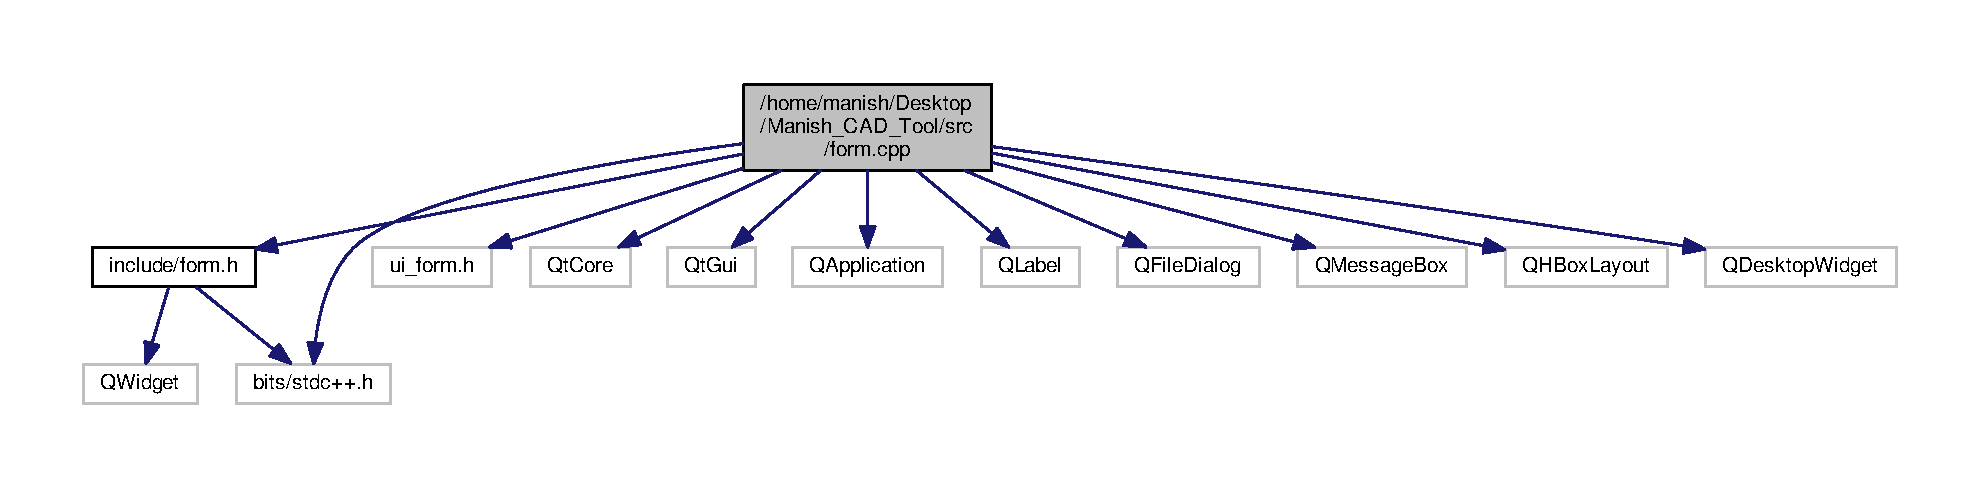
\includegraphics[width=350pt]{form_8cpp__incl}
\end{center}
\end{figure}
\subsection*{Macros}
\begin{DoxyCompactItemize}
\item 
\#define \hyperlink{form_8cpp_a42257a545daf5b7933d6e8f96adc74f2}{F}~first
\item 
\#define \hyperlink{form_8cpp_af933676109efed7ab34cea71d748a517}{S}~second
\item 
\#define \hyperlink{form_8cpp_a276c5a0e984cf60015b27252fe04fe6b}{pb}~push\+\_\+back
\end{DoxyCompactItemize}


\subsection{Macro Definition Documentation}
\index{form.\+cpp@{form.\+cpp}!F@{F}}
\index{F@{F}!form.\+cpp@{form.\+cpp}}
\subsubsection[{\texorpdfstring{F}{F}}]{\setlength{\rightskip}{0pt plus 5cm}\#define F~first}\hypertarget{form_8cpp_a42257a545daf5b7933d6e8f96adc74f2}{}\label{form_8cpp_a42257a545daf5b7933d6e8f96adc74f2}


Definition at line 19 of file form.\+cpp.

\index{form.\+cpp@{form.\+cpp}!pb@{pb}}
\index{pb@{pb}!form.\+cpp@{form.\+cpp}}
\subsubsection[{\texorpdfstring{pb}{pb}}]{\setlength{\rightskip}{0pt plus 5cm}\#define pb~push\+\_\+back}\hypertarget{form_8cpp_a276c5a0e984cf60015b27252fe04fe6b}{}\label{form_8cpp_a276c5a0e984cf60015b27252fe04fe6b}


Definition at line 21 of file form.\+cpp.

\index{form.\+cpp@{form.\+cpp}!S@{S}}
\index{S@{S}!form.\+cpp@{form.\+cpp}}
\subsubsection[{\texorpdfstring{S}{S}}]{\setlength{\rightskip}{0pt plus 5cm}\#define S~second}\hypertarget{form_8cpp_af933676109efed7ab34cea71d748a517}{}\label{form_8cpp_af933676109efed7ab34cea71d748a517}


Definition at line 20 of file form.\+cpp.


\hypertarget{_full__plane_8cpp}{}\section{/home/manish/\+Desktop/\+Manish\+\_\+\+C\+A\+D\+\_\+\+Tool/src/\+Full\+\_\+plane.cpp File Reference}
\label{_full__plane_8cpp}\index{/home/manish/\+Desktop/\+Manish\+\_\+\+C\+A\+D\+\_\+\+Tool/src/\+Full\+\_\+plane.\+cpp@{/home/manish/\+Desktop/\+Manish\+\_\+\+C\+A\+D\+\_\+\+Tool/src/\+Full\+\_\+plane.\+cpp}}
{\ttfamily \#include \char`\"{}include/\+Full\+\_\+plane.\+h\char`\"{}}\\*
{\ttfamily \#include \char`\"{}include/general\+\_\+methods.\+h\char`\"{}}\\*
{\ttfamily \#include $<$cmath$>$}\\*
Include dependency graph for Full\+\_\+plane.\+cpp\+:
\nopagebreak
\begin{figure}[H]
\begin{center}
\leavevmode
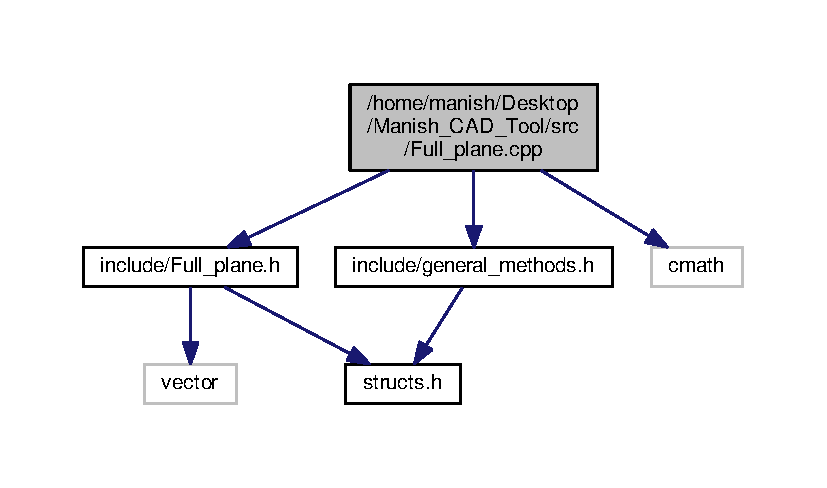
\includegraphics[width=350pt]{_full__plane_8cpp__incl}
\end{center}
\end{figure}
\subsection*{Macros}
\begin{DoxyCompactItemize}
\item 
\#define \hyperlink{_full__plane_8cpp_a06b50f1ca7258a9862c39d3ed354bf7c}{epsilon}~0.\+000001
\end{DoxyCompactItemize}


\subsection{Macro Definition Documentation}
\index{Full\+\_\+plane.\+cpp@{Full\+\_\+plane.\+cpp}!epsilon@{epsilon}}
\index{epsilon@{epsilon}!Full\+\_\+plane.\+cpp@{Full\+\_\+plane.\+cpp}}
\subsubsection[{\texorpdfstring{epsilon}{epsilon}}]{\setlength{\rightskip}{0pt plus 5cm}\#define epsilon~0.\+000001}\hypertarget{_full__plane_8cpp_a06b50f1ca7258a9862c39d3ed354bf7c}{}\label{_full__plane_8cpp_a06b50f1ca7258a9862c39d3ed354bf7c}


Definition at line 4 of file Full\+\_\+plane.\+cpp.


\hypertarget{general__methods_8cpp}{}\section{/home/manish/\+Desktop/\+Manish\+\_\+\+C\+A\+D\+\_\+\+Tool/src/general\+\_\+methods.cpp File Reference}
\label{general__methods_8cpp}\index{/home/manish/\+Desktop/\+Manish\+\_\+\+C\+A\+D\+\_\+\+Tool/src/general\+\_\+methods.\+cpp@{/home/manish/\+Desktop/\+Manish\+\_\+\+C\+A\+D\+\_\+\+Tool/src/general\+\_\+methods.\+cpp}}
{\ttfamily \#include \char`\"{}include/general\+\_\+methods.\+h\char`\"{}}\\*
Include dependency graph for general\+\_\+methods.\+cpp\+:
\nopagebreak
\begin{figure}[H]
\begin{center}
\leavevmode
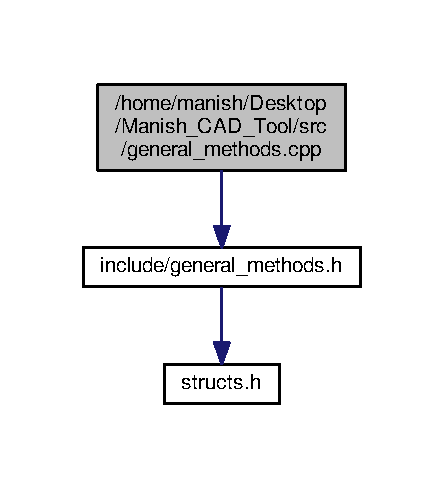
\includegraphics[width=213pt]{general__methods_8cpp__incl}
\end{center}
\end{figure}
\subsection*{Functions}
\begin{DoxyCompactItemize}
\item 
\hyperlink{classvertex__3d}{vertex\+\_\+3d} \hyperlink{general__methods_8cpp_a2dc9a47107e3f17fb944f6077f942236}{cross\+\_\+product} (\hyperlink{classvertex__3d}{vertex\+\_\+3d} a, \hyperlink{classvertex__3d}{vertex\+\_\+3d} b)
\item 
float \hyperlink{general__methods_8cpp_adde63ba9542357791cc6a967f2ea582e}{dot\+\_\+product} (\hyperlink{classvertex__3d}{vertex\+\_\+3d} a, \hyperlink{classvertex__3d}{vertex\+\_\+3d} b)
\end{DoxyCompactItemize}


\subsection{Function Documentation}
\index{general\+\_\+methods.\+cpp@{general\+\_\+methods.\+cpp}!cross\+\_\+product@{cross\+\_\+product}}
\index{cross\+\_\+product@{cross\+\_\+product}!general\+\_\+methods.\+cpp@{general\+\_\+methods.\+cpp}}
\subsubsection[{\texorpdfstring{cross\+\_\+product(vertex\+\_\+3d a, vertex\+\_\+3d b)}{cross_product(vertex_3d a, vertex_3d b)}}]{\setlength{\rightskip}{0pt plus 5cm}{\bf vertex\+\_\+3d} cross\+\_\+product (
\begin{DoxyParamCaption}
\item[{{\bf vertex\+\_\+3d}}]{a, }
\item[{{\bf vertex\+\_\+3d}}]{b}
\end{DoxyParamCaption}
)}\hypertarget{general__methods_8cpp_a2dc9a47107e3f17fb944f6077f942236}{}\label{general__methods_8cpp_a2dc9a47107e3f17fb944f6077f942236}


Definition at line 5 of file general\+\_\+methods.\+cpp.

\index{general\+\_\+methods.\+cpp@{general\+\_\+methods.\+cpp}!dot\+\_\+product@{dot\+\_\+product}}
\index{dot\+\_\+product@{dot\+\_\+product}!general\+\_\+methods.\+cpp@{general\+\_\+methods.\+cpp}}
\subsubsection[{\texorpdfstring{dot\+\_\+product(vertex\+\_\+3d a, vertex\+\_\+3d b)}{dot_product(vertex_3d a, vertex_3d b)}}]{\setlength{\rightskip}{0pt plus 5cm}float dot\+\_\+product (
\begin{DoxyParamCaption}
\item[{{\bf vertex\+\_\+3d}}]{a, }
\item[{{\bf vertex\+\_\+3d}}]{b}
\end{DoxyParamCaption}
)}\hypertarget{general__methods_8cpp_adde63ba9542357791cc6a967f2ea582e}{}\label{general__methods_8cpp_adde63ba9542357791cc6a967f2ea582e}


Definition at line 17 of file general\+\_\+methods.\+cpp.


\hypertarget{main_8cpp}{}\section{/home/manish/\+Desktop/\+Manish\+\_\+\+C\+A\+D\+\_\+\+Tool/src/main.cpp File Reference}
\label{main_8cpp}\index{/home/manish/\+Desktop/\+Manish\+\_\+\+C\+A\+D\+\_\+\+Tool/src/main.\+cpp@{/home/manish/\+Desktop/\+Manish\+\_\+\+C\+A\+D\+\_\+\+Tool/src/main.\+cpp}}
{\ttfamily \#include \char`\"{}include/mainwindow.\+h\char`\"{}}\\*
{\ttfamily \#include $<$Q\+Application$>$}\\*
{\ttfamily \#include $<$iostream$>$}\\*
Include dependency graph for main.\+cpp\+:
\nopagebreak
\begin{figure}[H]
\begin{center}
\leavevmode
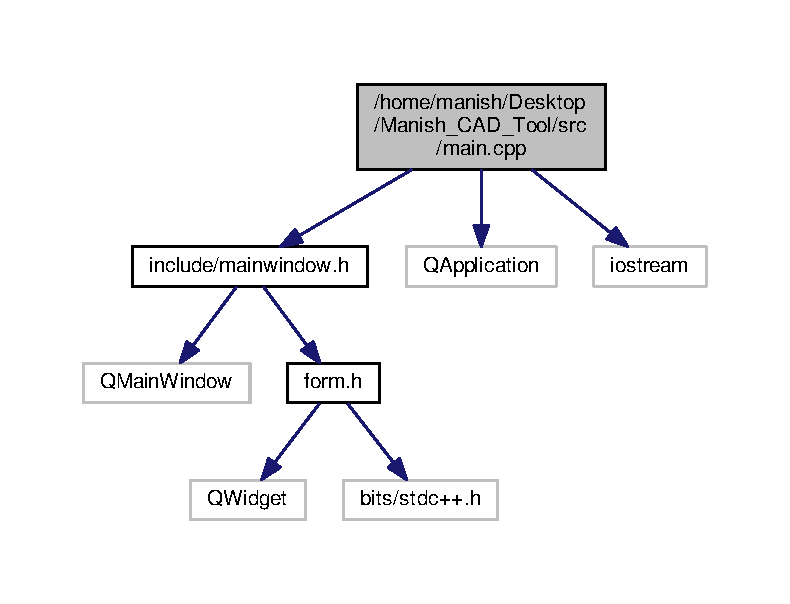
\includegraphics[width=350pt]{main_8cpp__incl}
\end{center}
\end{figure}
\subsection*{Functions}
\begin{DoxyCompactItemize}
\item 
int \hyperlink{main_8cpp_a0ddf1224851353fc92bfbff6f499fa97}{main} (int argc, char $\ast$argv\mbox{[}$\,$\mbox{]})
\end{DoxyCompactItemize}


\subsection{Function Documentation}
\index{main.\+cpp@{main.\+cpp}!main@{main}}
\index{main@{main}!main.\+cpp@{main.\+cpp}}
\subsubsection[{\texorpdfstring{main(int argc, char $\ast$argv[])}{main(int argc, char *argv[])}}]{\setlength{\rightskip}{0pt plus 5cm}int main (
\begin{DoxyParamCaption}
\item[{int}]{argc, }
\item[{char $\ast$}]{argv\mbox{[}$\,$\mbox{]}}
\end{DoxyParamCaption}
)}\hypertarget{main_8cpp_a0ddf1224851353fc92bfbff6f499fa97}{}\label{main_8cpp_a0ddf1224851353fc92bfbff6f499fa97}


Definition at line 6 of file main.\+cpp.


\hypertarget{mainwindow_8cpp}{}\section{/home/manish/\+Desktop/\+Manish\+\_\+\+C\+A\+D\+\_\+\+Tool/src/mainwindow.cpp File Reference}
\label{mainwindow_8cpp}\index{/home/manish/\+Desktop/\+Manish\+\_\+\+C\+A\+D\+\_\+\+Tool/src/mainwindow.\+cpp@{/home/manish/\+Desktop/\+Manish\+\_\+\+C\+A\+D\+\_\+\+Tool/src/mainwindow.\+cpp}}
{\ttfamily \#include \char`\"{}include/mainwindow.\+h\char`\"{}}\\*
{\ttfamily \#include \char`\"{}ui\+\_\+mainwindow.\+h\char`\"{}}\\*
{\ttfamily \#include \char`\"{}include/3d\+\_\+to\+\_\+2d.\+h\char`\"{}}\\*
{\ttfamily \#include \char`\"{}include/2d\+\_\+to\+\_\+3d.\+h\char`\"{}}\\*
{\ttfamily \#include \char`\"{}form.\+h\char`\"{}}\\*
{\ttfamily \#include $<$Q\+File\+Dialog$>$}\\*
{\ttfamily \#include $<$Q\+Message\+Box$>$}\\*
{\ttfamily \#include $<$iostream$>$}\\*
Include dependency graph for mainwindow.\+cpp\+:
\nopagebreak
\begin{figure}[H]
\begin{center}
\leavevmode
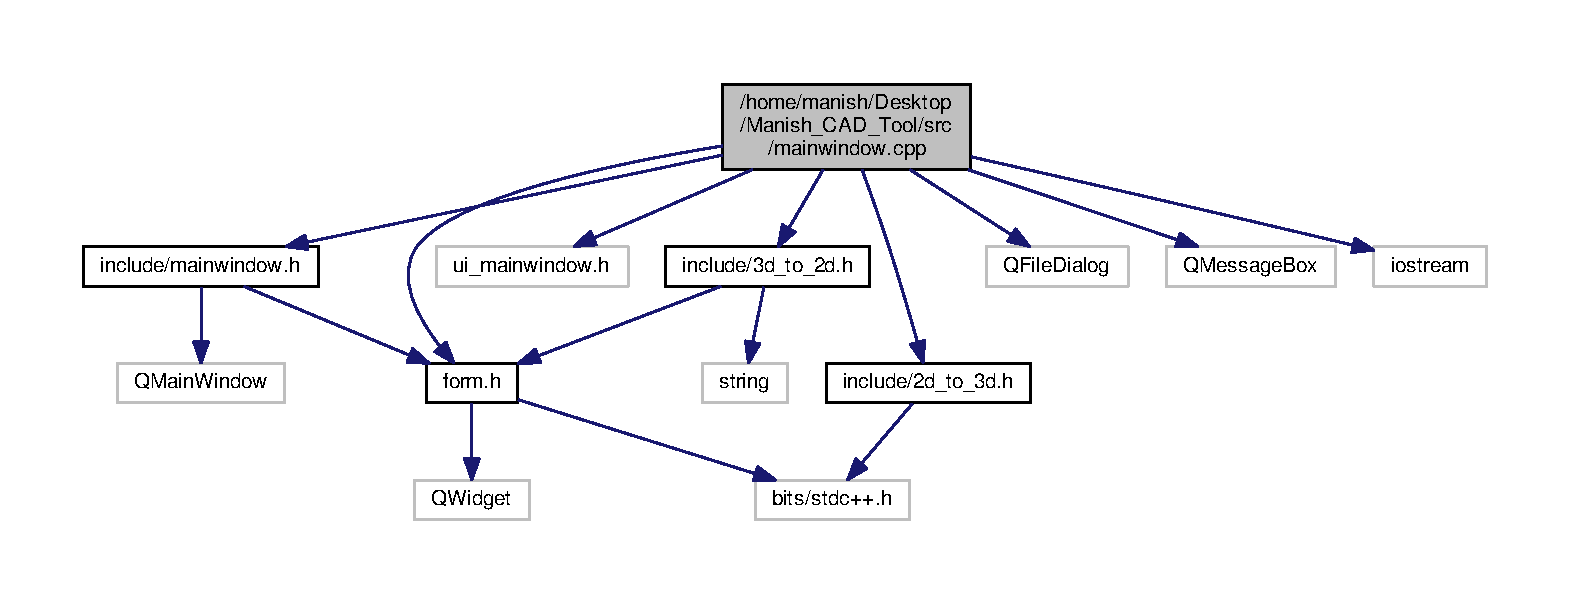
\includegraphics[width=350pt]{mainwindow_8cpp__incl}
\end{center}
\end{figure}
\subsection*{Variables}
\begin{DoxyCompactItemize}
\item 
std\+::string \hyperlink{mainwindow_8cpp_aba3248433c09cb10ab3f52f9d071fa8d}{file\+\_\+str}
\item 
std\+::string \hyperlink{mainwindow_8cpp_a95b24aa831523d475032130753a1cc07}{file\+\_\+outstr}
\end{DoxyCompactItemize}


\subsection{Variable Documentation}
\index{mainwindow.\+cpp@{mainwindow.\+cpp}!file\+\_\+outstr@{file\+\_\+outstr}}
\index{file\+\_\+outstr@{file\+\_\+outstr}!mainwindow.\+cpp@{mainwindow.\+cpp}}
\subsubsection[{\texorpdfstring{file\+\_\+outstr}{file_outstr}}]{\setlength{\rightskip}{0pt plus 5cm}std\+::string file\+\_\+outstr}\hypertarget{mainwindow_8cpp_a95b24aa831523d475032130753a1cc07}{}\label{mainwindow_8cpp_a95b24aa831523d475032130753a1cc07}


Definition at line 10 of file mainwindow.\+cpp.

\index{mainwindow.\+cpp@{mainwindow.\+cpp}!file\+\_\+str@{file\+\_\+str}}
\index{file\+\_\+str@{file\+\_\+str}!mainwindow.\+cpp@{mainwindow.\+cpp}}
\subsubsection[{\texorpdfstring{file\+\_\+str}{file_str}}]{\setlength{\rightskip}{0pt plus 5cm}std\+::string file\+\_\+str}\hypertarget{mainwindow_8cpp_aba3248433c09cb10ab3f52f9d071fa8d}{}\label{mainwindow_8cpp_aba3248433c09cb10ab3f52f9d071fa8d}


Definition at line 10 of file mainwindow.\+cpp.


\hypertarget{object__2d_8cpp}{}\section{/home/manish/\+Desktop/\+Manish\+\_\+\+C\+A\+D\+\_\+\+Tool/src/object\+\_\+2d.cpp File Reference}
\label{object__2d_8cpp}\index{/home/manish/\+Desktop/\+Manish\+\_\+\+C\+A\+D\+\_\+\+Tool/src/object\+\_\+2d.\+cpp@{/home/manish/\+Desktop/\+Manish\+\_\+\+C\+A\+D\+\_\+\+Tool/src/object\+\_\+2d.\+cpp}}
{\ttfamily \#include \char`\"{}include/object\+\_\+2d.\+h\char`\"{}}\\*
{\ttfamily \#include $<$iostream$>$}\\*
Include dependency graph for object\+\_\+2d.\+cpp\+:
\nopagebreak
\begin{figure}[H]
\begin{center}
\leavevmode
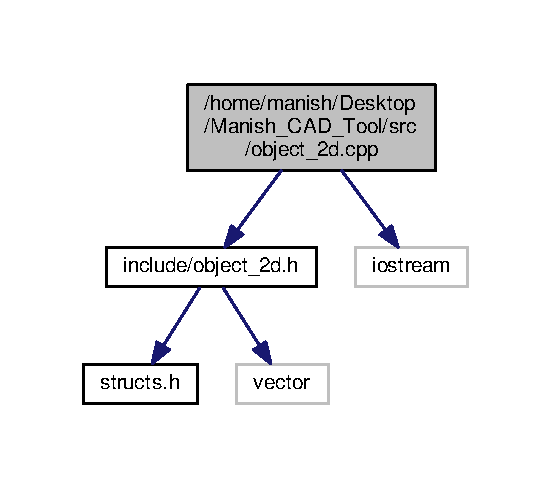
\includegraphics[width=265pt]{object__2d_8cpp__incl}
\end{center}
\end{figure}

\hypertarget{_object__3d_8cpp}{}\section{/home/manish/\+Desktop/\+Manish\+\_\+\+C\+A\+D\+\_\+\+Tool/src/\+Object\+\_\+3d.cpp File Reference}
\label{_object__3d_8cpp}\index{/home/manish/\+Desktop/\+Manish\+\_\+\+C\+A\+D\+\_\+\+Tool/src/\+Object\+\_\+3d.\+cpp@{/home/manish/\+Desktop/\+Manish\+\_\+\+C\+A\+D\+\_\+\+Tool/src/\+Object\+\_\+3d.\+cpp}}
{\ttfamily \#include \char`\"{}include/\+Object\+\_\+3d.\+h\char`\"{}}\\*
{\ttfamily \#include \char`\"{}include/general\+\_\+methods.\+h\char`\"{}}\\*
{\ttfamily \#include \char`\"{}include/planar\+\_\+graph\+\_\+generator.\+h\char`\"{}}\\*
{\ttfamily \#include \char`\"{}include/faceloop\+\_\+generator.\+h\char`\"{}}\\*
{\ttfamily \#include \char`\"{}include/body\+\_\+loop.\+h\char`\"{}}\\*
{\ttfamily \#include $<$algorithm$>$}\\*
{\ttfamily \#include $<$iostream$>$}\\*
{\ttfamily \#include $<$cmath$>$}\\*
{\ttfamily \#include $<$set$>$}\\*
Include dependency graph for Object\+\_\+3d.\+cpp\+:
\nopagebreak
\begin{figure}[H]
\begin{center}
\leavevmode
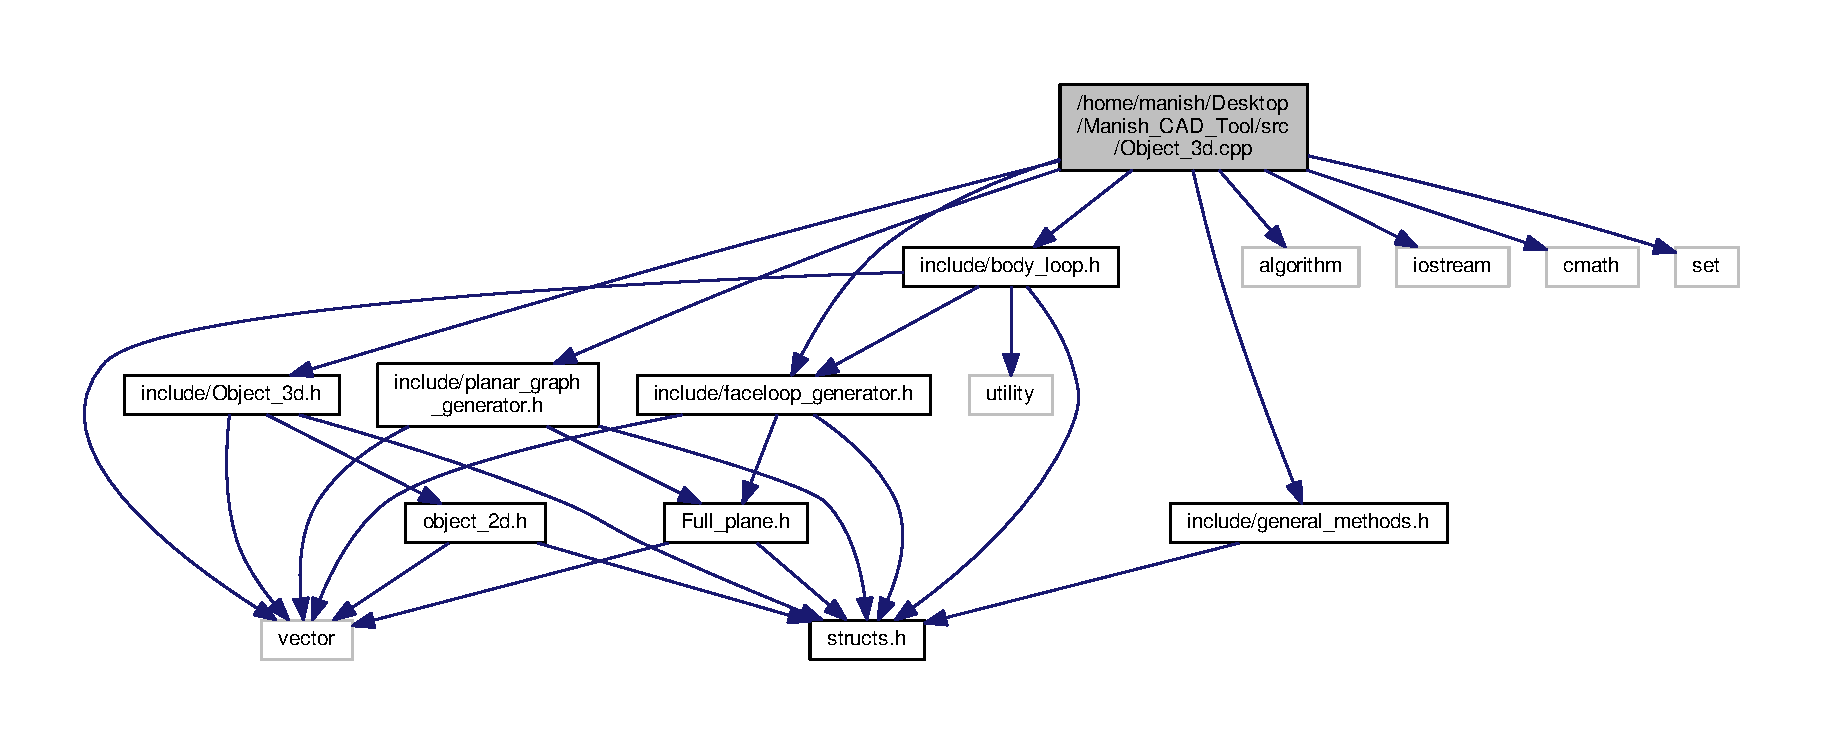
\includegraphics[width=350pt]{_object__3d_8cpp__incl}
\end{center}
\end{figure}
\subsection*{Macros}
\begin{DoxyCompactItemize}
\item 
\#define \hyperlink{_object__3d_8cpp_a06b50f1ca7258a9862c39d3ed354bf7c}{epsilon}~0.\+000001
\end{DoxyCompactItemize}
\subsection*{Functions}
\begin{DoxyCompactItemize}
\item 
bool \hyperlink{_object__3d_8cpp_a673d29e725926b7f236de4cac8549fb2}{compare} (pair$<$ \hyperlink{classvertex__2d}{vertex\+\_\+2d}, int $>$ \&lhs, pair$<$ \hyperlink{classvertex__2d}{vertex\+\_\+2d}, int $>$ \&rhs)
\end{DoxyCompactItemize}


\subsection{Macro Definition Documentation}
\index{Object\+\_\+3d.\+cpp@{Object\+\_\+3d.\+cpp}!epsilon@{epsilon}}
\index{epsilon@{epsilon}!Object\+\_\+3d.\+cpp@{Object\+\_\+3d.\+cpp}}
\subsubsection[{\texorpdfstring{epsilon}{epsilon}}]{\setlength{\rightskip}{0pt plus 5cm}\#define epsilon~0.\+000001}\hypertarget{_object__3d_8cpp_a06b50f1ca7258a9862c39d3ed354bf7c}{}\label{_object__3d_8cpp_a06b50f1ca7258a9862c39d3ed354bf7c}


Definition at line 11 of file Object\+\_\+3d.\+cpp.



\subsection{Function Documentation}
\index{Object\+\_\+3d.\+cpp@{Object\+\_\+3d.\+cpp}!compare@{compare}}
\index{compare@{compare}!Object\+\_\+3d.\+cpp@{Object\+\_\+3d.\+cpp}}
\subsubsection[{\texorpdfstring{compare(pair$<$ vertex\+\_\+2d, int $>$ \&lhs, pair$<$ vertex\+\_\+2d, int $>$ \&rhs)}{compare(pair< vertex_2d, int > &lhs, pair< vertex_2d, int > &rhs)}}]{\setlength{\rightskip}{0pt plus 5cm}bool compare (
\begin{DoxyParamCaption}
\item[{pair$<$ {\bf vertex\+\_\+2d}, int $>$ \&}]{lhs, }
\item[{pair$<$ {\bf vertex\+\_\+2d}, int $>$ \&}]{rhs}
\end{DoxyParamCaption}
)}\hypertarget{_object__3d_8cpp_a673d29e725926b7f236de4cac8549fb2}{}\label{_object__3d_8cpp_a673d29e725926b7f236de4cac8549fb2}


Definition at line 127 of file Object\+\_\+3d.\+cpp.


\hypertarget{planar__graph__generator_8cpp}{}\section{/home/manish/\+Desktop/\+Manish\+\_\+\+C\+A\+D\+\_\+\+Tool/src/planar\+\_\+graph\+\_\+generator.cpp File Reference}
\label{planar__graph__generator_8cpp}\index{/home/manish/\+Desktop/\+Manish\+\_\+\+C\+A\+D\+\_\+\+Tool/src/planar\+\_\+graph\+\_\+generator.\+cpp@{/home/manish/\+Desktop/\+Manish\+\_\+\+C\+A\+D\+\_\+\+Tool/src/planar\+\_\+graph\+\_\+generator.\+cpp}}
{\ttfamily \#include \char`\"{}include/planar\+\_\+graph\+\_\+generator.\+h\char`\"{}}\\*
{\ttfamily \#include \char`\"{}include/general\+\_\+methods.\+h\char`\"{}}\\*
{\ttfamily \#include $<$iostream$>$}\\*
Include dependency graph for planar\+\_\+graph\+\_\+generator.\+cpp\+:
\nopagebreak
\begin{figure}[H]
\begin{center}
\leavevmode
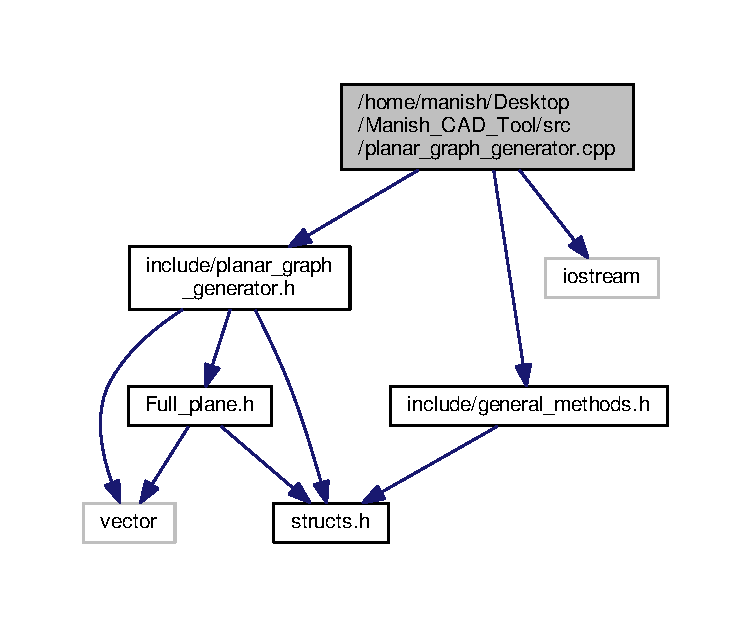
\includegraphics[width=350pt]{planar__graph__generator_8cpp__incl}
\end{center}
\end{figure}
\subsection*{Macros}
\begin{DoxyCompactItemize}
\item 
\#define \hyperlink{planar__graph__generator_8cpp_a06b50f1ca7258a9862c39d3ed354bf7c}{epsilon}~0.\+000001
\end{DoxyCompactItemize}
\subsection*{Functions}
\begin{DoxyCompactItemize}
\item 
std\+::vector$<$ \hyperlink{class_full__plane}{Full\+\_\+plane} $>$ \hyperlink{planar__graph__generator_8cpp_a2cdfdb8be2237b1c7359b630e9603cfd}{planar\+\_\+graph\+\_\+generator} (std\+::vector$<$ \hyperlink{classvertex__3d}{vertex\+\_\+3d} $>$ v3d\+\_\+list, std\+::vector$<$ \hyperlink{classedge__3d}{edge\+\_\+3d} $>$ \&e3d\+\_\+list)
\begin{DoxyCompactList}\small\item\em function that generates and retunrs planes \end{DoxyCompactList}\item 
std\+::vector$<$ \hyperlink{classplane}{plane} $>$ \hyperlink{planar__graph__generator_8cpp_a8d89f969b47445ac1b5b0cf170401cf1}{construct\+\_\+planes} (std\+::vector$<$ \hyperlink{classvertex__3d}{vertex\+\_\+3d} $>$ v3d\+\_\+list, std\+::vector$<$ \hyperlink{classedge__3d}{edge\+\_\+3d} $>$ e3d\+\_\+list, std\+::vector$<$ std\+::vector$<$ int $>$ $>$ adj\+\_\+list)
\begin{DoxyCompactList}\small\item\em function that constructs plane equations \end{DoxyCompactList}\item 
std\+::vector$<$ std\+::vector$<$ int $>$ $>$ \hyperlink{planar__graph__generator_8cpp_a077660a929dda9adf2f8a2daa6a563c1}{get\+\_\+adj\+\_\+list} (std\+::vector$<$ \hyperlink{classedge__3d}{edge\+\_\+3d} $>$ e3d\+\_\+list, int no\+\_\+of\+\_\+vertices)
\begin{DoxyCompactList}\small\item\em function that returns adjacency edges list of the \hyperlink{classvertex__3d}{vertex\+\_\+3d} list \end{DoxyCompactList}\item 
std\+::vector$<$ \hyperlink{classplane}{plane} $>$ \hyperlink{planar__graph__generator_8cpp_a488a27459d11af0b73b76ebe78a8a1c4}{eliminate\+\_\+duplicate\+\_\+planes} (std\+::vector$<$ \hyperlink{classplane}{plane} $>$ planes)
\begin{DoxyCompactList}\small\item\em function that eliminates duplicate formed planes \end{DoxyCompactList}\item 
bool \hyperlink{planar__graph__generator_8cpp_acd37db477f3dd31a46790f5a7ded851c}{check\+\_\+legality} (\hyperlink{class_full__plane}{Full\+\_\+plane} \&f, std\+::vector$<$ std\+::vector$<$ int $>$ $>$ adj\+\_\+list)
\begin{DoxyCompactList}\small\item\em function returns true if planar graph is legal \end{DoxyCompactList}\item 
void \hyperlink{planar__graph__generator_8cpp_a47eedebb44f45567710e54702a5f28b6}{remove\+\_\+dangling} (\hyperlink{class_full__plane}{Full\+\_\+plane} \&f, std\+::vector$<$ std\+::vector$<$ int $>$ $>$ adj\+\_\+list)
\begin{DoxyCompactList}\small\item\em function that removes dangling and isolated edges on the planar graph using dfs \end{DoxyCompactList}\item 
void \hyperlink{planar__graph__generator_8cpp_ad4d8aa255999d941dcc6b5b61ca9d0fd}{remove\+\_\+single\+\_\+plane\+\_\+edges} (std\+::vector$<$ \hyperlink{class_full__plane}{Full\+\_\+plane} $>$ \&f\+\_\+list, std\+::vector$<$ \hyperlink{classedge__3d}{edge\+\_\+3d} $>$ \&e3d\+\_\+list)
\begin{DoxyCompactList}\small\item\em function that removes those edges which belongs only to one planner graph \end{DoxyCompactList}\end{DoxyCompactItemize}


\subsection{Macro Definition Documentation}
\index{planar\+\_\+graph\+\_\+generator.\+cpp@{planar\+\_\+graph\+\_\+generator.\+cpp}!epsilon@{epsilon}}
\index{epsilon@{epsilon}!planar\+\_\+graph\+\_\+generator.\+cpp@{planar\+\_\+graph\+\_\+generator.\+cpp}}
\subsubsection[{\texorpdfstring{epsilon}{epsilon}}]{\setlength{\rightskip}{0pt plus 5cm}\#define epsilon~0.\+000001}\hypertarget{planar__graph__generator_8cpp_a06b50f1ca7258a9862c39d3ed354bf7c}{}\label{planar__graph__generator_8cpp_a06b50f1ca7258a9862c39d3ed354bf7c}


Definition at line 5 of file planar\+\_\+graph\+\_\+generator.\+cpp.



\subsection{Function Documentation}
\index{planar\+\_\+graph\+\_\+generator.\+cpp@{planar\+\_\+graph\+\_\+generator.\+cpp}!check\+\_\+legality@{check\+\_\+legality}}
\index{check\+\_\+legality@{check\+\_\+legality}!planar\+\_\+graph\+\_\+generator.\+cpp@{planar\+\_\+graph\+\_\+generator.\+cpp}}
\subsubsection[{\texorpdfstring{check\+\_\+legality(\+Full\+\_\+plane \&f, std\+::vector$<$ std\+::vector$<$ int $>$ $>$ adj\+\_\+list)}{check_legality(Full_plane &f, std::vector< std::vector< int > > adj_list)}}]{\setlength{\rightskip}{0pt plus 5cm}bool check\+\_\+legality (
\begin{DoxyParamCaption}
\item[{{\bf Full\+\_\+plane} \&}]{f, }
\item[{std\+::vector$<$ std\+::vector$<$ int $>$ $>$}]{adj\+\_\+list}
\end{DoxyParamCaption}
)}\hypertarget{planar__graph__generator_8cpp_acd37db477f3dd31a46790f5a7ded851c}{}\label{planar__graph__generator_8cpp_acd37db477f3dd31a46790f5a7ded851c}


function returns true if planar graph is legal 



Definition at line 80 of file planar\+\_\+graph\+\_\+generator.\+cpp.

\index{planar\+\_\+graph\+\_\+generator.\+cpp@{planar\+\_\+graph\+\_\+generator.\+cpp}!construct\+\_\+planes@{construct\+\_\+planes}}
\index{construct\+\_\+planes@{construct\+\_\+planes}!planar\+\_\+graph\+\_\+generator.\+cpp@{planar\+\_\+graph\+\_\+generator.\+cpp}}
\subsubsection[{\texorpdfstring{construct\+\_\+planes(std\+::vector$<$ vertex\+\_\+3d $>$ v3d\+\_\+list, std\+::vector$<$ edge\+\_\+3d $>$ e3d\+\_\+list, std\+::vector$<$ std\+::vector$<$ int $>$ $>$ adj\+\_\+list)}{construct_planes(std::vector< vertex_3d > v3d_list, std::vector< edge_3d > e3d_list, std::vector< std::vector< int > > adj_list)}}]{\setlength{\rightskip}{0pt plus 5cm}std\+::vector$<$ {\bf plane} $>$ construct\+\_\+planes (
\begin{DoxyParamCaption}
\item[{std\+::vector$<$ {\bf vertex\+\_\+3d} $>$}]{v3d\+\_\+list, }
\item[{std\+::vector$<$ {\bf edge\+\_\+3d} $>$}]{e3d\+\_\+list, }
\item[{std\+::vector$<$ std\+::vector$<$ int $>$ $>$}]{adj\+\_\+list}
\end{DoxyParamCaption}
)}\hypertarget{planar__graph__generator_8cpp_a8d89f969b47445ac1b5b0cf170401cf1}{}\label{planar__graph__generator_8cpp_a8d89f969b47445ac1b5b0cf170401cf1}


function that constructs plane equations 



Definition at line 27 of file planar\+\_\+graph\+\_\+generator.\+cpp.

\index{planar\+\_\+graph\+\_\+generator.\+cpp@{planar\+\_\+graph\+\_\+generator.\+cpp}!eliminate\+\_\+duplicate\+\_\+planes@{eliminate\+\_\+duplicate\+\_\+planes}}
\index{eliminate\+\_\+duplicate\+\_\+planes@{eliminate\+\_\+duplicate\+\_\+planes}!planar\+\_\+graph\+\_\+generator.\+cpp@{planar\+\_\+graph\+\_\+generator.\+cpp}}
\subsubsection[{\texorpdfstring{eliminate\+\_\+duplicate\+\_\+planes(std\+::vector$<$ plane $>$ planes)}{eliminate_duplicate_planes(std::vector< plane > planes)}}]{\setlength{\rightskip}{0pt plus 5cm}std\+::vector$<$ {\bf plane} $>$ eliminate\+\_\+duplicate\+\_\+planes (
\begin{DoxyParamCaption}
\item[{std\+::vector$<$ {\bf plane} $>$}]{planes}
\end{DoxyParamCaption}
)}\hypertarget{planar__graph__generator_8cpp_a488a27459d11af0b73b76ebe78a8a1c4}{}\label{planar__graph__generator_8cpp_a488a27459d11af0b73b76ebe78a8a1c4}


function that eliminates duplicate formed planes 



Definition at line 57 of file planar\+\_\+graph\+\_\+generator.\+cpp.

\index{planar\+\_\+graph\+\_\+generator.\+cpp@{planar\+\_\+graph\+\_\+generator.\+cpp}!get\+\_\+adj\+\_\+list@{get\+\_\+adj\+\_\+list}}
\index{get\+\_\+adj\+\_\+list@{get\+\_\+adj\+\_\+list}!planar\+\_\+graph\+\_\+generator.\+cpp@{planar\+\_\+graph\+\_\+generator.\+cpp}}
\subsubsection[{\texorpdfstring{get\+\_\+adj\+\_\+list(std\+::vector$<$ edge\+\_\+3d $>$ e3d\+\_\+list, int no\+\_\+of\+\_\+vertices)}{get_adj_list(std::vector< edge_3d > e3d_list, int no_of_vertices)}}]{\setlength{\rightskip}{0pt plus 5cm}std\+::vector$<$ std\+::vector$<$int$>$ $>$ get\+\_\+adj\+\_\+list (
\begin{DoxyParamCaption}
\item[{std\+::vector$<$ {\bf edge\+\_\+3d} $>$}]{e3d\+\_\+list, }
\item[{int}]{no\+\_\+of\+\_\+vertices}
\end{DoxyParamCaption}
)}\hypertarget{planar__graph__generator_8cpp_a077660a929dda9adf2f8a2daa6a563c1}{}\label{planar__graph__generator_8cpp_a077660a929dda9adf2f8a2daa6a563c1}


function that returns adjacency edges list of the \hyperlink{classvertex__3d}{vertex\+\_\+3d} list 



Definition at line 49 of file planar\+\_\+graph\+\_\+generator.\+cpp.

\index{planar\+\_\+graph\+\_\+generator.\+cpp@{planar\+\_\+graph\+\_\+generator.\+cpp}!planar\+\_\+graph\+\_\+generator@{planar\+\_\+graph\+\_\+generator}}
\index{planar\+\_\+graph\+\_\+generator@{planar\+\_\+graph\+\_\+generator}!planar\+\_\+graph\+\_\+generator.\+cpp@{planar\+\_\+graph\+\_\+generator.\+cpp}}
\subsubsection[{\texorpdfstring{planar\+\_\+graph\+\_\+generator(std\+::vector$<$ vertex\+\_\+3d $>$ v3d\+\_\+list, std\+::vector$<$ edge\+\_\+3d $>$ \&e3d\+\_\+list)}{planar_graph_generator(std::vector< vertex_3d > v3d_list, std::vector< edge_3d > &e3d_list)}}]{\setlength{\rightskip}{0pt plus 5cm}std\+::vector$<$ {\bf Full\+\_\+plane} $>$ planar\+\_\+graph\+\_\+generator (
\begin{DoxyParamCaption}
\item[{std\+::vector$<$ {\bf vertex\+\_\+3d} $>$}]{v3d\+\_\+list, }
\item[{std\+::vector$<$ {\bf edge\+\_\+3d} $>$ \&}]{e3d\+\_\+list}
\end{DoxyParamCaption}
)}\hypertarget{planar__graph__generator_8cpp_a2cdfdb8be2237b1c7359b630e9603cfd}{}\label{planar__graph__generator_8cpp_a2cdfdb8be2237b1c7359b630e9603cfd}


function that generates and retunrs planes 



Definition at line 8 of file planar\+\_\+graph\+\_\+generator.\+cpp.

\index{planar\+\_\+graph\+\_\+generator.\+cpp@{planar\+\_\+graph\+\_\+generator.\+cpp}!remove\+\_\+dangling@{remove\+\_\+dangling}}
\index{remove\+\_\+dangling@{remove\+\_\+dangling}!planar\+\_\+graph\+\_\+generator.\+cpp@{planar\+\_\+graph\+\_\+generator.\+cpp}}
\subsubsection[{\texorpdfstring{remove\+\_\+dangling(\+Full\+\_\+plane \&f, std\+::vector$<$ std\+::vector$<$ int $>$ $>$ adj\+\_\+list)}{remove_dangling(Full_plane &f, std::vector< std::vector< int > > adj_list)}}]{\setlength{\rightskip}{0pt plus 5cm}void remove\+\_\+dangling (
\begin{DoxyParamCaption}
\item[{{\bf Full\+\_\+plane} \&}]{f, }
\item[{std\+::vector$<$ std\+::vector$<$ int $>$ $>$}]{adj\+\_\+list}
\end{DoxyParamCaption}
)}\hypertarget{planar__graph__generator_8cpp_a47eedebb44f45567710e54702a5f28b6}{}\label{planar__graph__generator_8cpp_a47eedebb44f45567710e54702a5f28b6}


function that removes dangling and isolated edges on the planar graph using dfs 



Definition at line 90 of file planar\+\_\+graph\+\_\+generator.\+cpp.

\index{planar\+\_\+graph\+\_\+generator.\+cpp@{planar\+\_\+graph\+\_\+generator.\+cpp}!remove\+\_\+single\+\_\+plane\+\_\+edges@{remove\+\_\+single\+\_\+plane\+\_\+edges}}
\index{remove\+\_\+single\+\_\+plane\+\_\+edges@{remove\+\_\+single\+\_\+plane\+\_\+edges}!planar\+\_\+graph\+\_\+generator.\+cpp@{planar\+\_\+graph\+\_\+generator.\+cpp}}
\subsubsection[{\texorpdfstring{remove\+\_\+single\+\_\+plane\+\_\+edges(std\+::vector$<$ Full\+\_\+plane $>$ \&f\+\_\+list, std\+::vector$<$ edge\+\_\+3d $>$ \&e3d\+\_\+list)}{remove_single_plane_edges(std::vector< Full_plane > &f_list, std::vector< edge_3d > &e3d_list)}}]{\setlength{\rightskip}{0pt plus 5cm}void remove\+\_\+single\+\_\+plane\+\_\+edges (
\begin{DoxyParamCaption}
\item[{std\+::vector$<$ {\bf Full\+\_\+plane} $>$ \&}]{f\+\_\+list, }
\item[{std\+::vector$<$ {\bf edge\+\_\+3d} $>$ \&}]{e3d\+\_\+list}
\end{DoxyParamCaption}
)}\hypertarget{planar__graph__generator_8cpp_ad4d8aa255999d941dcc6b5b61ca9d0fd}{}\label{planar__graph__generator_8cpp_ad4d8aa255999d941dcc6b5b61ca9d0fd}


function that removes those edges which belongs only to one planner graph 



Definition at line 121 of file planar\+\_\+graph\+\_\+generator.\+cpp.


\hypertarget{structs_8cpp}{}\section{/home/manish/\+Desktop/\+Manish\+\_\+\+C\+A\+D\+\_\+\+Tool/src/structs.cpp File Reference}
\label{structs_8cpp}\index{/home/manish/\+Desktop/\+Manish\+\_\+\+C\+A\+D\+\_\+\+Tool/src/structs.\+cpp@{/home/manish/\+Desktop/\+Manish\+\_\+\+C\+A\+D\+\_\+\+Tool/src/structs.\+cpp}}
{\ttfamily \#include \char`\"{}include/structs.\+h\char`\"{}}\\*
{\ttfamily \#include $<$cmath$>$}\\*
{\ttfamily \#include $<$iostream$>$}\\*
Include dependency graph for structs.\+cpp\+:
\nopagebreak
\begin{figure}[H]
\begin{center}
\leavevmode
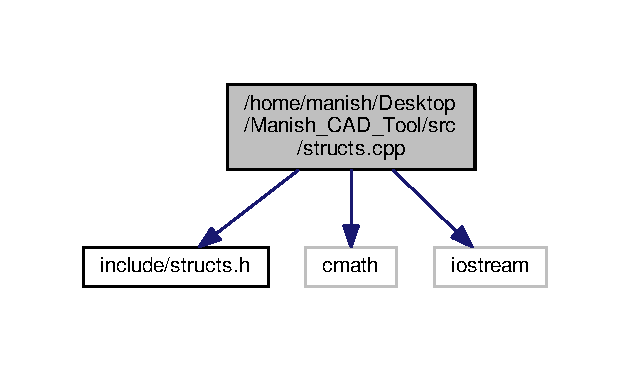
\includegraphics[width=303pt]{structs_8cpp__incl}
\end{center}
\end{figure}
\subsection*{Macros}
\begin{DoxyCompactItemize}
\item 
\#define \hyperlink{structs_8cpp_a06b50f1ca7258a9862c39d3ed354bf7c}{epsilon}~0.\+000001
\end{DoxyCompactItemize}


\subsection{Macro Definition Documentation}
\index{structs.\+cpp@{structs.\+cpp}!epsilon@{epsilon}}
\index{epsilon@{epsilon}!structs.\+cpp@{structs.\+cpp}}
\subsubsection[{\texorpdfstring{epsilon}{epsilon}}]{\setlength{\rightskip}{0pt plus 5cm}\#define epsilon~0.\+000001}\hypertarget{structs_8cpp_a06b50f1ca7258a9862c39d3ed354bf7c}{}\label{structs_8cpp_a06b50f1ca7258a9862c39d3ed354bf7c}


Definition at line 3 of file structs.\+cpp.


%--- End generated contents ---

% Index
\backmatter
\newpage
\phantomsection
\clearemptydoublepage
\addcontentsline{toc}{chapter}{Index}
\printindex

\end{document}
